\documentclass{prose}

\newcounter{problemcounter}
\usepackage{tcolorbox}
\newenvironment{assignment}[1]
  {
    \refstepcounter{problemcounter}
    \begin{tcolorbox}[colback=black!3!white,colframe=black!15!white,coltitle=black,fonttitle=\bfseries,title=Aufgabe \theproblemcounter --- #1,arc=0mm,toprule=0.2mm,bottomrule=0.2mm,leftrule=0.2mm,rightrule=0.2mm,left=1mm,right=1mm,titlerule=0mm,middle=0.5mm]
  }
  {
    \end{tcolorbox}
  }

\title{Mitschrieb Elementare Geometrie}
\author{Jens Ochsenmeier \& Maximilian Franz \& Nadine Schorpp}

\begin{document}

  \maketitle

  \tableofcontents

  % chapters
  \chapter{Einstieg --- Metrische Räume}

\section{Vorbemerkungen}

Inhalt dieser Vorlesung wird sowohl \emph{Stetigkeitsgeometrie} (Topologie) als auch \emph{metrische Geometrie} sein. Die unten abgebildeten Objekte sind im Sinne der Stetigkeitsgeometrie "topologisch äquivalent", im Sinne der metrischen Geometrie sind diese allerdings verschieden.

\begin{figure}[H]
  \label{img003-1}
  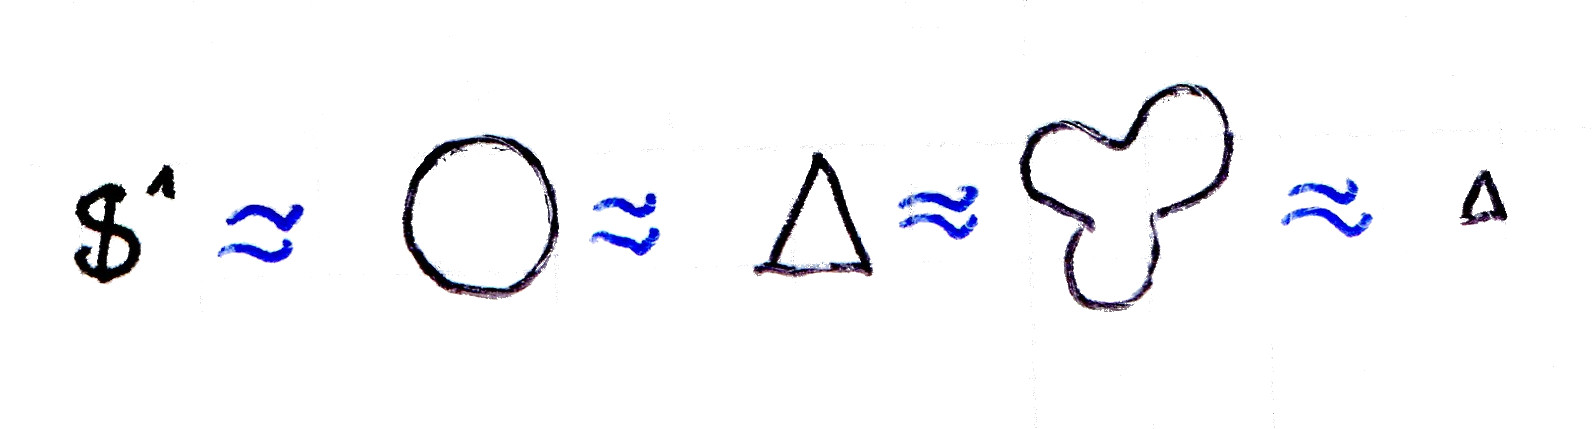
\includegraphics{img003-1}
  \caption{Diese Objekte sind topologisch äquivalent, metrisch allerdings nicht}
\end{figure}

\begin{remark}[Kartographieproblem]
  Ein zentrales Problem der Kartographie ist die \emph{längentreue} Abbildung einer Fläche auf der Weltkugel auf eine Fläche auf Papier. Mithilfe der Differentialgeometrie und der Gauß-Krümmung lässt sich zeigen, dass das nicht möglich ist.
\end{remark}

\section{Definitionen zu metrischen Räumen}

\begin{definition}[Metrik]
  \label{def:metrik}
  Sei $ X $ eine Menge. Eine Funktion $ d: X \times X \to \R_{\geq 0} $ ist eine \term{Metrik} (Abstandsfunktion), falls $ \forall x, y, z \in X $ gilt:
  \begin{enumerate}
    \item \textbf{Positivität}: $ d(x, y) = 0 \Leftrightarrow x = y $ 
    \item \textbf{Symmetrie}: $ d(x,y) = d(y,x) $
    \item \textbf{Dreiecksungleichung}: $ d(x,z) \leq d(x,y) + d(y,z) $
  \end{enumerate}
\end{definition}

\begin{definition}[Metrischer Raum]
  \label{def:metrischerRaum}
  Ein \term{metrischer Raum} ist ein Paar $ (X,d) $ aus einer Menge und einer \hyperref[def:metrik]{Metrik} auf dieser.
\end{definition}

\begin{definition}[Pseudometrik]
  \label{def:pseudometrik}
  Eine \term{Pseudometrik} erfüllt die gleichen Bedingungen wie eine \hyperref[def:metrik]{Metrik}, außer $ d(x,y) = 0 \Rightarrow x = y $ --- die Umkehrung gilt.
\end{definition}

\begin{definition}[Abgeschlossener $ r $-Ball um $ x $]
  \label{def:abgeschlossenerBall}
  Eine Teilmenge
  \begin{equation*}
    \overline{B_r(x)} \coloneqq \{ y \in X : d(x,y) \leq r \}
  \end{equation*}
  heißt \term{abgeschlossener $ r $-Ball um $ x $}.
\end{definition}

\begin{definition}[Abstandserhaltende Abbildung]
  \label{def:abstandserhaltendeAbbildung}
  Sind $ (X, d_X) $ und $ (Y, d_Y) $ \hyperref[def:metrischerRaum]{metrische Räume}, so heißt eine Abbildung $ f: X \to Y $ \term{abstandserhaltend}, falls
  \begin{equation*}
    \forall x, y \in X: d_Y(f(x), f(y)) = d_X(x, y)\text{.}
  \end{equation*}
\end{definition}

\begin{definition}[Isometrie] 
  \label{def:isometrie}
  Eine \term{Isometrie} ist eine bijektive \hyperref[def:abstandserhaltendeAbbildung]{abstandserhaltende Abbildung}. Falls eine Isometrie
  \begin{equation*}
    f: (X, d_X) \to (Y, d_Y)
  \end{equation*}
  existiert, so heißen $ X $ und $ Y $ \emph{isometrisch}.
\end{definition}

\section{Beispiele zu metrischen Räumen}

\begin{example}[Triviale Metrik]
  \label{bsp:trivialeMetrik}
  Menge $ X $,
  \begin{equation*}
    d(x, y) \coloneqq \begin{cases}
    0, &x = y \\
    1, & x \neq y
  \end{cases}\text{,}
  \end{equation*}
  also lässt mithilfe der \term{trivialen Metrik} jede Menge zu einem \hyperref[def:metrischerRaum]{metrischen Raum} verwursten. 
\end{example}

\begin{example}[Simple {\hyperref[def:metrik]{Metriken}}]
  \label{bsp:simpleMetriken}
  Sei $ X = \R $.\footnote{\textbf{Anmerkung}: Wenn $ d(x, y) $ eine \hyperref[def:metrik]{Metrik} ist, so ist auch $ \widetilde{d}(x, y) \coloneqq \lambda d(x, y) $ mit $ \lambda \in \R_{>0} $ eine Metrik.}
  \begin{itemize}
    \item $ d_1(s, t) \coloneqq |s-t| $ ist Metrik.
    \item $ d_2(s, t) \coloneqq \log(|s-t|+1) $ ist Metrik.
  \end{itemize}
\end{example}

\begin{example}[Euklidische Standardmetrik]
  \label{bsp:standardmetrik}
  $ X = \R^n $,
  \begin{equation*}
    d_e(x, y) \coloneqq \sqrt{\sum_{i=1}^n(x_i-y_i)^2} = \Vert x-y \Vert
  \end{equation*}
  ist die \term{(euklidische) Standardmetrik} auf dem $ \R^n $. Die Dreiecksungleichung folgt aus der Cauchy-Schwarz-Ungleichung\footnote{\textbf{Cauchy-Schwarz-Ungleichung}: $ \langle x, y \rangle \leq ||x||*||y|| \quad (x, y \in \R) $}.
\end{example}

\begin{remark}[aus LA II]
  \hyperref[def:isometrie]{Isometrien} von $ (\R^n, d_e) $ sind Translationen, Rotationen und Spiegelungen.
\end{remark}

\begin{example}[Maximumsmetrik]
  \label{bsp:maximumsmetrik}
  $ X = \R $,
  \begin{equation*}
    d(x, y) \coloneqq \underset{1 \leq i \leq n}{\max} \vert x_i-y_i \vert
  \end{equation*}
  ist \hyperref[def:metrik]{Metrik}.
\end{example}

\begin{example}[{\hyperref[bsp:standardmetrik]{Standardmetrik}} und {\hyperref[bsp:maximumsmetrik]{Maximumsmetrik}} allgemein: Norm]
  \label{bsp:norm}
  $ V $ sei $ \R $-Vektorraum. Eine \term{Norm} auf $ V $ ist eine Abbildung 
  \begin{equation*}
    \Vert\cdot\Vert : V \to \R_{>0}\text{,}
  \end{equation*}
  so dass $ \forall v, w \in V, \lambda \in \R $:
  \begin{enumerate}
    \item \textbf{Definitheit}: $ ||v|| = 0 \Leftrightarrow v = 0 $
    \item \textbf{absolute Homogenität}: $ ||\lambda v|| = |\lambda| * ||v|| $
    \item \textbf{Dreiecksungleichung}: $ ||v+w|| \leq ||v||+||w|| $
  \end{enumerate}
  Eine Norm definiert eine \hyperref[def:metrik]{Metrik} durch $ d(v, w) \coloneqq ||v-w|| $.
\end{example}

\begin{example}[Einheitssphäre]
  \label{bsp:einheitssphaere}
  \begin{equation*}
    S_1^n \coloneqq \{ x \in \R^{n+1} : ||x|| = 1 \}
  \end{equation*}
  ist die $ n $-te \term{Einheitssphäre}. \\
  Auf dieser ist mit
  \begin{equation*}
     d_W(x, y) \coloneqq \arccos(\langle x, y \rangle)
  \end{equation*}
  die \term{Winkel-Metrik} definiert.

  \begin{figure}[H]
    \label{img004-1}
    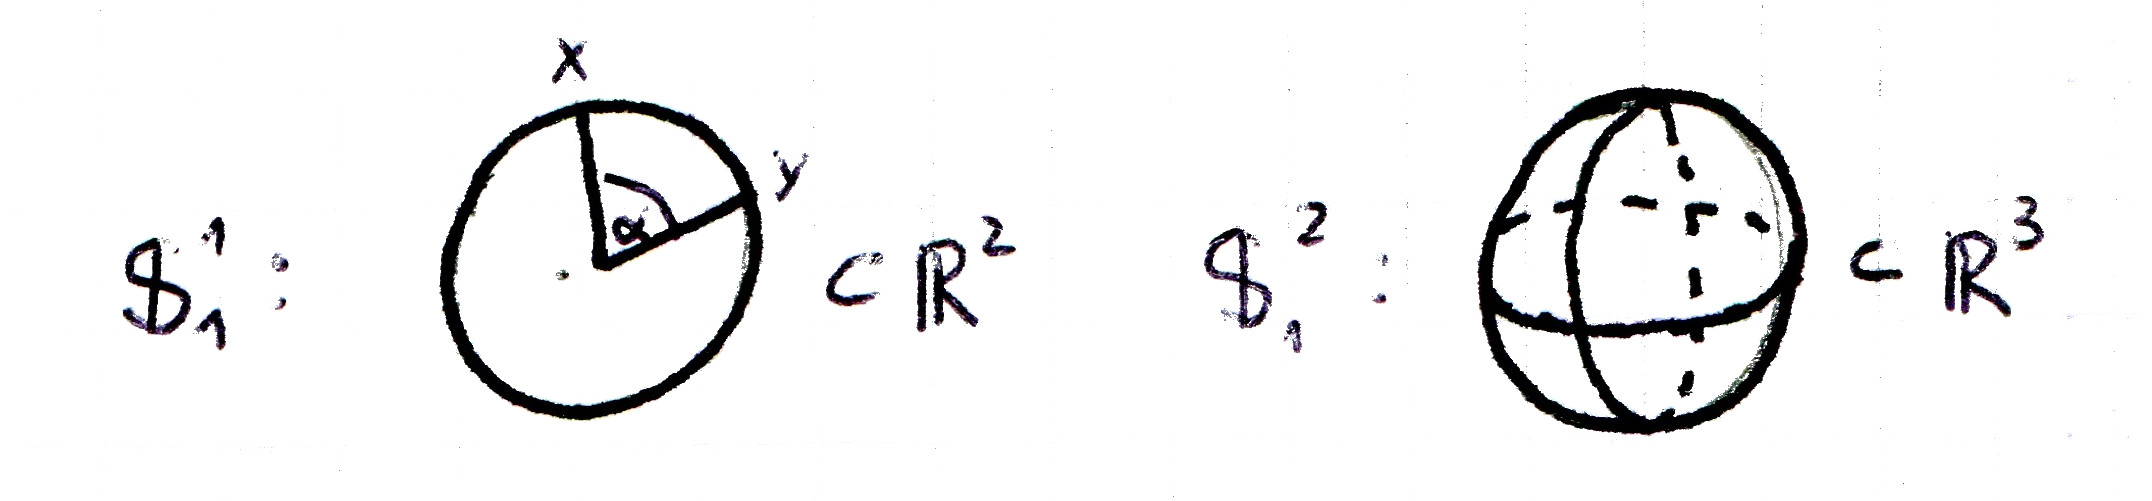
\includegraphics[width=.5\textwidth]{img004-1}
    \caption{Die erste und zweite Einheitssphäre}
  \end{figure}
\end{example}

\begin{example}(Hamming-Metrik)
  Es ist $ \mathbb{F}_2 $ der Körper mit zwei Elementen $ \{ 0, 1 \} $,
  \begin{equation*}
    X \coloneqq \mathbb{F}_2^n = \{ (f_1, \dots, f_n) : f_i = 0 \vee f_i = 1 \ (i \in {1, \dots, n}) \}
  \end{equation*}
  die Menge der binären Zahlenfolgen der Länge $ n $. Die \term{Hamming-Metrik} ist definiert als
  \begin{equation*}
    d_H: X \times X \to \R_{>0}, \quad d_H(u,v) = |\{ i : u_i \neq v_i \}|\text{.}
  \end{equation*}
\end{example}
  \chapter{Längenmetriken}

\section{Graphen}

\begin{definition}[Graph]
  \label{def:graph}
  Ein \term{Graph} $ G = (E, K) $ besteht aus einer \emph{Ecken}-Menge $ E $ und einer Menge von Paaren $ \{ u, v \} $ ($ u, v \in E $), genannt \emph{Kanten}.
\end{definition}

\begin{definition}[Erreichbarkeit]
  Seien $ p, q \in E $ von $ G = (E, K) $. $ q $ ist \term{erreichbar} von $ p $ aus, falls ein \emph{Kantenzug} von $ p $ nach $ q $ existiert.
\end{definition}

\begin{definition}[Zusammenhängend]
  $ G = (E, K) $ heißt \term{zusammenhängend}, falls alle Ecken von einer beliebigen, festen Ecke aus erreichbar sind.
  \\
  Ist $ G $ ein zusammenhängender \hyperref[def:graph]{Graph}, so ist $ d(p, q) = $ minimale Kantenzahl eines Kantenzuges von $ p $ nach $ q $ eine \hyperref[def:metrik]{Metrik}.
\end{definition}

\begin{example}[Wortmetrik]
  Sei $ \Gamma \coloneqq \langle S \rangle $ vom endlichen Erzeugendensystem $ S $ erzeugte Gruppe. Dann:
  \begin{equation}
    \label{gl:wortmetrik}
    g \in \Gamma \Rightarrow g = s_1\cdot \dots s_n\text{ (multiplikativ, nicht eindeutig),}
  \end{equation}
  z.B. $ \Z = \langle \pm 1 \rangle $. \\
  Dann lässt sich über die Länge von $ g \in \Gamma $ (minimales $ n $ in \autoref{gl:wortmetrik}) eine \hyperref[def:metrik]{Metrik} definieren:
\end{example}

\begin{definition}[Wortmetrik]
  \label{def:wortmetrik}
  \begin{equation*}
    d_S(g, k) \coloneqq |g^{-1}k|
  \end{equation*}
  ist eine \hyperref[def:metrik]{Metrik} mit
  \begin{align*}
    d_s(kg,kh) &= |(kg)^{-1}kh| \\ 
    &= |g^{-1}\underbrace{k^{-1}k}_{=e}h| = |g^{-1}h| \\
    &= d_s(g,h)\text{,}
  \end{align*}
  also ist $ d_s $ linksmultiplikativ mit $ k \in \Gamma $ und damit eine \hyperref[def:isometrie]{Isometrie}.
\end{definition}

\begin{definition}[Cayley-Graph]
  Der \term{Cayley-Graph} $ \text{Cay}(\Gamma, S) $ von $ \Gamma $ bezüglich $ S $ ist der Graph $ G = (E, K) $ mit
  \begin{equation*}
    E \coloneqq \Gamma, \quad K \coloneqq \{ (g, gs) : g \in \Gamma, s \in S \}\text{.}
  \end{equation*}
  Die \emph{Graphen-Metrik} auf $ \text{Cay}(\Gamma, S) $ ist \hyperref[def:isometrie]{isometrisch} zur \hyperref[def:wortmetrik]{Wortmetrik}.
\end{definition}

\section{Euklidische Metrik}
\begin{example}[Euklidische Metrik auf $ \R^2 $ als Standardmetrik]
  Sei
  \begin{equation*}
    c : [a,b] \to \R^2, \quad t \mapsto (x(t), y(t))
  \end{equation*}
  eine stückweise differenzierbare\footnote{\textbf{Hinweis}: Mit \emph{differenzierbar} ist im Folgenden immer $ C^\infty $-differenzierbar gemeint, wenn nicht anders angegeben.} Kurve.
  Die \emph{euklidische Länge} von $ C $ ist
  \begin{align*}
    L_{\text{euk}}(c) &\coloneqq \int_a^b \Vert C'(t) \Vert dt \quad \text{(via \emph{Polynom-Approximation})} \\
     &= \int_a^b \sqrt{\left( x'(t) \right)^2 + \left( y'(t) \right)^2}dt\text{.}
  \end{align*}
  \begin{figure}[H]
    \label{img006-1}
    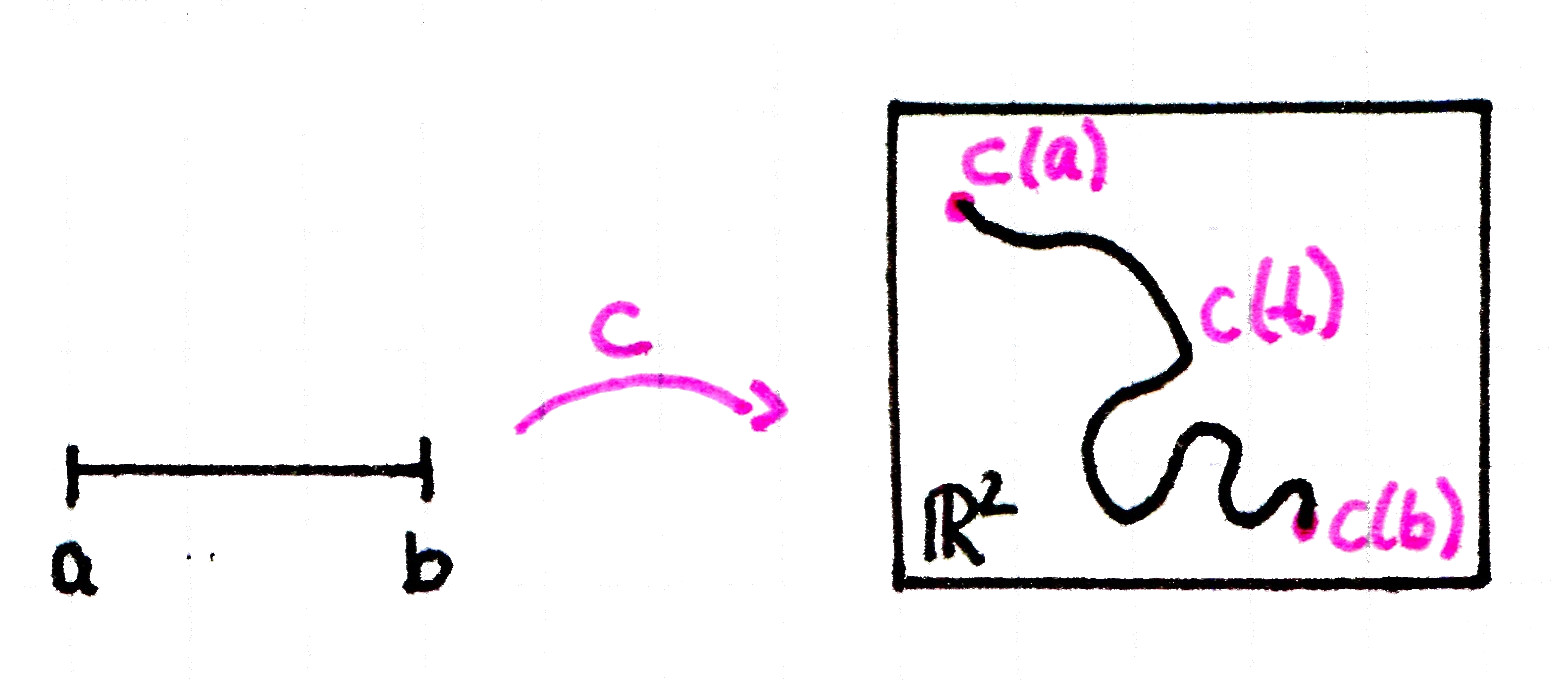
\includegraphics[width=.5\textwidth]{img006-1}
    \caption{Eine stückweise differenzierbare Kurve im $ \R^2 $}
  \end{figure}
  \emph{Beispiel}: Geraden-Segment.
  \begin{equation*}
    g: [0,1] \to \R^2, \quad t \mapsto g(t) = (1-t)p + tq\text{.}
  \end{equation*}
  Dann:
  \begin{equation*}
    g'(t) = -p+q, \quad \Vert g'(t) \Vert = \Vert p - q \Vert
  \end{equation*}
  und damit
  \begin{equation*}
    \underline{L_{\text{euk}}(g)} = \int_0^1\Vert p - q \Vert dt = \Vert p - q \Vert = \underline{d_e(p,q)}\text{.}
  \end{equation*}
\end{example}

\begin{lemma}[Unabhängigkeit von $ \text{L}_\text{euk} $]
  \label{lm:leuklinvarianz} \
  \begin{enumerate}
    \item $ L_\text{euk}(c) $ ist unabhängig von Kurvenparametrisierung.
    \item $ L_\text{euk}(c) $ ist invariant unter Translationen, Drehungen und Spiegelungen.
  \end{enumerate}
  \begin{proof}
    \
    \begin{enumerate}
      \item Zu zeigen: Für $ c: [a,b] \to \R^2 $, $ t \mapsto c(t) $ und einen monoton wachsenden Diffeomorphismus\footnote{\textbf{Diffeomorphismus}: Bijektive, stetig differenzierbare Abbildung, deren Umkehrabbildung auch stetig differenzierbar ist.} $ t: [c, d] \to [a,b] $, $ s \mapsto t(s) $ gilt:
      \begin{equation*}
        L_\text{euk}(c(t(s))) = L_\text{euk}(c(t))\text{.}
      \end{equation*}
      Das folgt unmittelbar aus der Substitutionsregel für Integrale:
      \begin{equation*}
        \int_c^d \left\Vert \frac{dc}{ds} \right\Vert ds = \int_c^d \left\Vert \frac{d_c(t(s))}{dt} \right\Vert \frac{dt}{ds}ds = \int_{t(c) = a}^{t(d)=b} \left\Vert \frac{dc}{dt} \right\Vert dt \text{.}
      \end{equation*}\qed
      \item \begin{itemize}
        \item \underline{Translation}. \\ Für $ p = (p_1, \dots, p_n) \in \R^2 $ sei
        \begin{equation*}
           T_p(c(t)) = c(t) + p = (\lambda(t) + p_1, y(t) + p_2)
         \end{equation*} 
         die von $ p $ verschobene Kurve. Es gilt
         \begin{equation*}
           (T_p \circ c)(t) = c'(t) \Rightarrow \int_a^b \left\Vert (T_p \circ c)' \right\Vert dt = \int_a^b \left\Vert c' \right\Vert dt
         \end{equation*}
         und damit gilt das Lemma für Translationen. \qed
        \item \underline{Drehung}. \\
        Für $ \theta \in [0,2\pi] $ sei
        \begin{align*}
          D_\theta \circ c(t) &= \begin{pmatrix}
            \cos\theta & -\sin\theta \\
            \sin\theta & \cos\theta
          \end{pmatrix}c(t) \\ 
           &= (\cos\theta x(t) - \sin\theta y(t), \sin\theta x(t) + \cos\theta y(t))
        \end{align*}
        die um Winkel $ \theta $ gedrehte Kurve. \\
        Da $ D_\theta $ eine orthogonale Abbildung ist, folgt
        \begin{equation*}
          (D_\theta \circ c(t))' = D_\theta * c'(t)
        \end{equation*}
        und damit
        \begin{equation*}
          \left\Vert (D_\theta \circ c(t))' \right\Vert = \left\Vert D_\theta * c' \right\Vert \overset{\text{orth.}}{=} \left\Vert c' \right\Vert
        \end{equation*}
        und damit gilt das Lemma für Drehungen. \qed
        \item Spiegelungen sind wie Drehungen orthogonal, ihre Invarianz folgt aus der Invarianz der Drehungen.
      \end{itemize}
    \end{enumerate}
  \end{proof}
\end{lemma}

\begin{lemma}[Geraden sind am kürzesten]
  \label{lemma:geradenkurz}
  Die kürzesten Verbindungskurven zwischen Punkten in $ \R^2 $ sind genau die Geradensegmente. \\
  \begin{proof}
    \ \\
    \begin{minipage}{.45\textwidth}
      Seien $ p, q \in \R^2 $ beliebig. Durch geeignete Rotation und Translation kann man $ (p,q) $ überführen in Punkte in spezieller Lage;
      \begin{equation*}
        p' = (0,0), \quad q' = (0,l)\text{.}
      \end{equation*}
      Wegen \hyperref[lm:leuklinvarianz]{der Invarianz von $ L_\text{euk} $} ändert sich dabei die Länge entsprechender Verbindungskurven nicht. \\
      Sei jetzt $ c(t) \coloneqq (x(t),y(t)) $ eine stückweise differenzierbare Kurve zwischen $ p' $ und $ q' $. Dann gilt:
    \end{minipage}
    \hfill
    \begin{minipage}{.45\textwidth}
      \begin{figure}[H]
        \label{img007-1}
        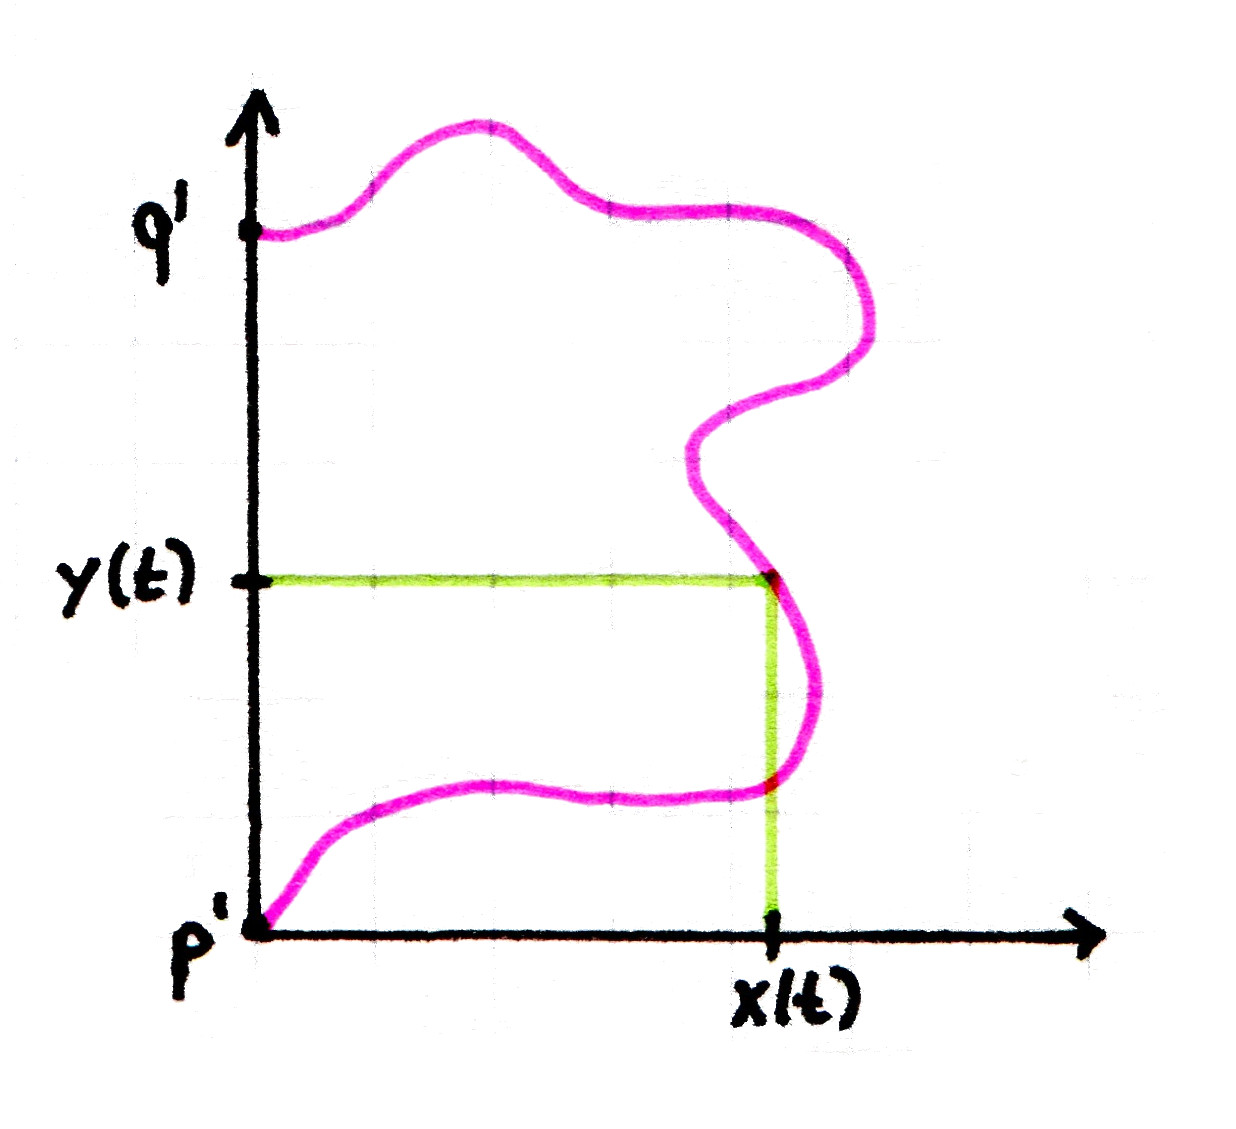
\includegraphics[width=.8\textwidth]{img007-1}
        \caption{Die ``geeignete'' Rotation einer Kurve, sodass Start- und Endpunkt auf einer Achse liegen}
      \end{figure}
    \end{minipage}
    \begin{align*}
      L_\text{euk}(c) &= \int_a^b\sqrt{(x')^2+(y')^2}dt \geq \int_a^b\vert y' \vert dt \geq \int_a^by'(t)dt = \int_{y(a) = 0}^{y(b) = l} dy \\
       &= l\text{.}
    \end{align*}
    $ l $ ist die Länge des Geradensegmentes zwischen $ p' $ und $ q' $. \\
    $ \Rightarrow $ \underline{Infimum} der Längenwerte wird angenommen. Eindeutigkeit bleibt zu zeigen. \\
    Gilt für eine Kurve $ c $, dass $ L_\text{euk}(c) = l $, so hat man in obigen Ungleichungen überall Gleichheit, also insbesondere $ x'(t) = 0 $ ($ \forall t $), also $ x(t) = \text{konstant} = x(0) = 0 $ und somit $ \widetilde{c} = (0,y(t)) $. Also ist $ \widetilde{c} $ auch (parametrisiertes) Geradensegment. \qed
  \end{proof}
\end{lemma}

\begin{definition}[Euklidische Metrik auf $ \R^2 $-Kurven]
  Für $ p,q \in \R^2 $ sei $ \Omega_{pq}(\R^2) $ die Menge der stetig differenzierbaren Verbindungskurven zwischen $ p $ und $ q $. Wir setzen dann:
  \begin{equation*}
    (p,q) = \inf L_\text{euk}(c), \quad c \in \Omega_{pq}(\R^2)\text{.}
  \end{equation*}
\end{definition}

\begin{theorem}[``Neuer'' \ metrischer $ \R^2 $]
  \begin{equation*}
    (\R^2, d_\text{euk})
  \end{equation*}
  ist ein \hyperref[def:metrischerRaum]{metrischer Raum} und \hyperref[def:isometrie]{isometrisch} zu $ (\R^2, d_e) $.
  \begin{proof}
    Direkter Beweis nach dem \hyperref[lemma:geradenkurz]{Lemma über Geradensegmente}. \\
    Man hat eine explizite Formel
    \begin{equation*}
      d_{\text{euk}}(p,q) = \Vert p - q \Vert = d_e(p,q)\text{.}
    \end{equation*}
    Die Identität ist eine Isometrie.
  \end{proof}
  \begin{proof}
    Konzeptioneller, allgemeinerer Beweis. Es werden die Metrik-Eigenschaften gezeigt.

    \begin{itemize}
      \item \emph{Symmetrie}. \\
        Sei
        \begin{equation*}
          \Omega_{pq}(\R^2) \ni c: [a,b] \to \R^2\text{.}
       \end{equation*}
       Idee: Kurve wird rückwärts durchlaufen. \\
       Es ist $ d_\text{e} = d_\text{euk} $, denn ist $ \widetilde{c}(t) = (a+b-t) \in \Omega_{qp}(\R^2) $ (mit gleicher Länge wie $ c $) und die Abbildung $ c \mapsto \widetilde{c} $ ist bijektiv. Dann $ L(\widetilde{c}) = L(c) $, und damit
       \begin{equation*}
         d(q,p) = \inf(L(\widetilde{c})) = \inf(L(c)) = d(p,q)\text{.}
       \end{equation*}

      \begin{minipage}{.45\textwidth}
        \item \emph{Dreiecksungleichung}. \\
          Zu zeigen: $ d_\text{euk}(p,q) \leq d_\text{euk}(p,r) + d_\text{euk}(r,q) $ ($ \forall p, q, r \in \R^2 $). \\
          Verknüpfen von Wegen von $ p $ nach $ r $ mit solchen von $ r $ nach $ q $ liefert gewisse --- aber i.A. nicht alle --- Wege von $ p $ nach $ q $:
          \begin{equation*}
            \Omega_{pr} \cup \Omega_{rq} \subsetneq \Omega_{pq}\text{.}
          \end{equation*}
          Infimumbildung liefert die Behauptung.
      \end{minipage}
      \hfill
      \begin{minipage}{.45\textwidth}
        \begin{figure}[H]
          \label{img008-1}
          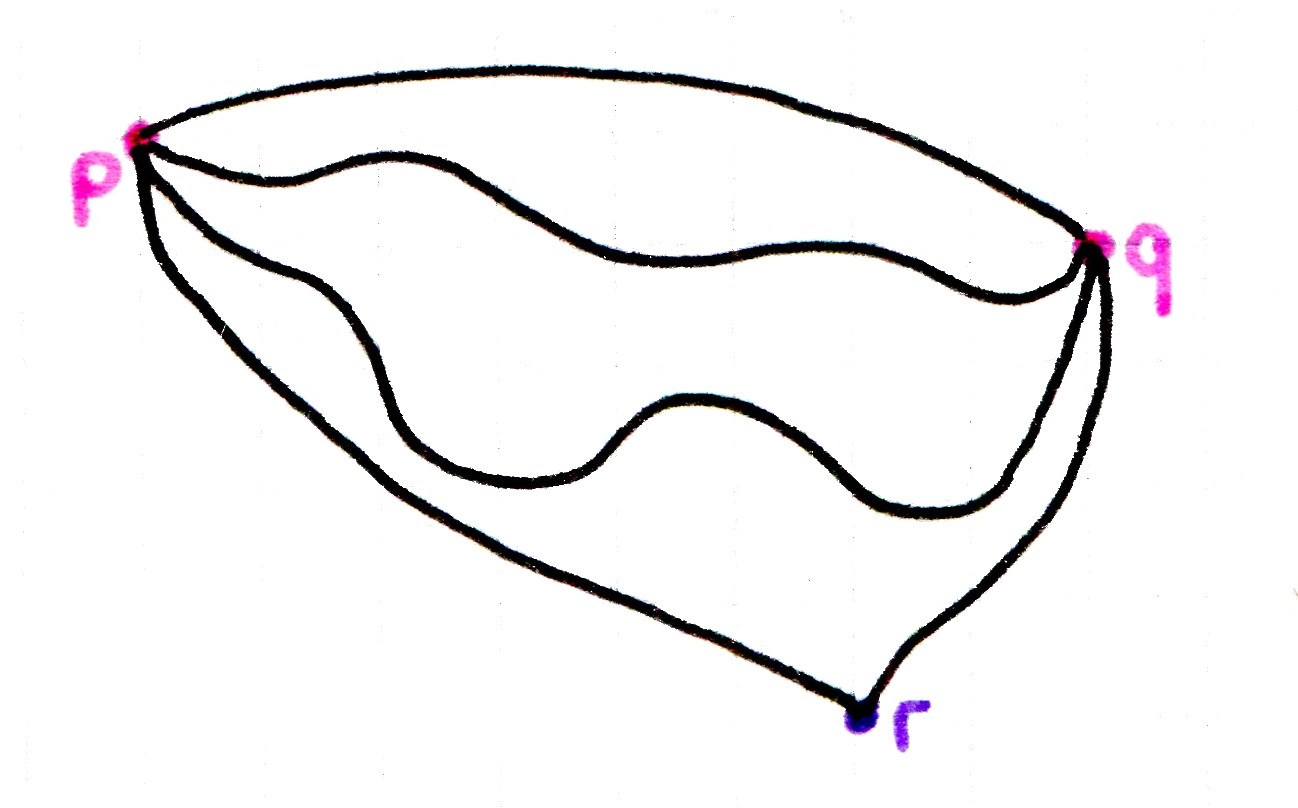
\includegraphics[width=.8\textwidth]{img008-1}
          \caption{Betrachte Wege von $ p $ nach $ q $ über $ r $ und nicht über $ r $}
        \end{figure}
      \end{minipage}

      \begin{minipage}{.45\textwidth}
        \item \emph{Positivität}. \\
          Zu zeigen: $ d_\text{euk}(p,q) = 0 \Leftrightarrow p = q $.
          \begin{itemize}
            \item Falls $ p = q $. \\
              Die konstante Kurve $ c: [0,1] \to \R^2, t \mapsto c(t) = p $ hat 
              \begin{equation*}
                c'(t) = 0 \Rightarrow L_\text{euk}(c) = 0 \leadsto d_\text{euk}(p,p) = 0 \text{.}
              \end{equation*}
            \item Falls $ p \neq q $. \\
              Die kürzeste Kurve ist das Geradensegment\footnotemark
              \begin{equation*}
                t \mapsto (1-t)p + tq
              \end{equation*}
              mit der Länge $ d_\text{euk} = \Vert p - q \Vert = 0 $.
          \end{itemize}
      \end{minipage}
      \footnotetext{\textbf{Anmerkung}: nur an dieser Stelle wird die Geometrie des $ \R^2 $ benötigt!}
      \hfill
      \begin{minipage}{.45\textwidth}
        \begin{figure}[H]
          \label{img008-1}
          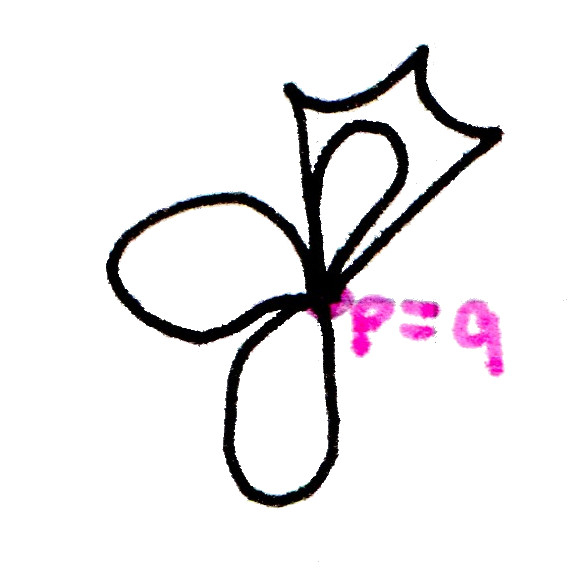
\includegraphics[width=.5\textwidth]{img008-2}
          \caption{``Schleifen''}
        \end{figure}
      \end{minipage}
    \end{itemize}
  \end{proof}
\end{theorem}

\section{Sphärische Geometrie}
\begin{example}[2-dimensionale sphärische Geometrie als Längenraum]
  Eine $ 2 $-dimensionale Sphäre von Radius $ R $ in $ \R^3 $ ist
  \begin{equation*}
    S^2_\R \coloneqq \{ x \in R^3 : \Vert x \Vert = R \} = \{ (x_1, x_2, x_3) \in \R^3 : x_1^2+x_2^2+x_3^2 = R^2 \}\text{.}
  \end{equation*}
  Für eine stückweise differenzierbare Kurve
  \begin{equation*}
    c: [a,b] \to S^2_\R \subset \R^3, \ t \mapsto (x_1(t), x_2(t), x_3(t))
  \end{equation*}
  definiere die \term{sphärische Länge} durch
  \begin{equation*}
    L_S(c) \coloneqq \int_a^b \Vert c'(t) \Vert dt = \int_a^b \sqrt{{x'}_1^2+{x'}_2^2+{x'}_3^2}dt
  \end{equation*}
  und
  \begin{equation*}
    d_s(p,q) \coloneqq \inf L_s(c) \quad (c \in \Omega_{pq}(S^2_\R))\text{.}
  \end{equation*}
\end{example}

\begin{lemma}[Kurvenlängen rotationsinvariant]
  \label{lemma:kurvenlaengen}
  Die Länge einer differenzierbaren Kurve auf $ S^2_\R $ ist invariant unter Rotationen von $ \R^2 $.
  \begin{proof}
    Eine orthogonale Matrix im $ \R^2 $ ist (bzgl. Standardbasis) gegeben durch eine orthogonale Matrix $ D \in \R^{2 \times 2} $. Da $ \Vert D(x) \Vert = \Vert x \Vert $ für $ x \in \R^3 $ gilt, ist $ D(S^2_\R) = S^2_\R $. Insbesondere ist für eine Kurve $ c $ in $ S^2_\R $ auch das Bild $ D \circ c \subset S^2_\R $. \\
    Weiter folgt aus $ (D \circ c(t))' = D \circ c'(t) $:
    \begin{align*}
      L_s(D \circ c) &= \int_a^b \Vert (D \circ c(t))' \Vert dt = \int_a^b \Vert D(c'(t)) \Vert dt \\
        &= \int_a^b \Vert c'(t) \Vert dt = L_S(c)\text{.}
    \end{align*}
  \end{proof}
\end{lemma}

\begin{lemma}[Großkreise sind am kürzesten]
  Die kürzesten Verbindungskurven zwischen zwei Punkten in $ S^2_\R $ sind \term{Großkreise}, also Schnitte von $ S^2_\R $ und zweidimensionalen Untervektorräumen des $ \R^3 $.
  \begin{proof}
    Seien zwei beliebige Punkte $ p,q $ auf $ S^2_\R $. Dann finden wir eine Rotation von $ \R^3 $, die $ p $ auf $ p' = (0,0,R) $ --- also den ``Nordpol'' --- und $ q $ auf $ q' = (0,y,z) \in S^2_\R $ abbildet. Aufgrund der \hyperref[lemma:kurvenlaengen]{Rotationsinvarianz der Kurvenlängen} und der Definition ist $ d_s(p,q) = d_s(p', q') $. Es genügt also eine kürzeste Verbindung zwischen $ p' $ und $ q' $ zu finden. \\
    \emph{Idee}: Mittels ``geographischer Koordinaten'' $ \varphi $ und $ \theta $. Nun kann eine Verbindung zwischen $ p' $ und $ q' $ geschrieben werden als
    \begin{equation*}
      c(t) = R(\sin\theta(t)\cos\varphi(t), \ \sin\theta(t)\sin\varphi(t), \ \cos\theta(t))
    \end{equation*}
    und somit
    \begin{small}
      \begin{equation*}
        c'(t) = (\theta'\cos\theta\cos\varphi-\varphi'\sin\theta\sin\varphi, \ \theta'\cos\theta\sin\varphi+\varphi'\sin\theta\cos\varphi, \ -\theta'\sin\theta)\text{,}
      \end{equation*}
    \end{small}
    also
    \begin{equation*}
      \Vert c'(t) \Vert = R^2({\theta'}^2 + {\varphi'}^2\sin^2\theta)
    \end{equation*}
    und somit
    \begin{align*}
      L_s(c) &= R\int_a^b\sqrt{{\theta'}^2+{\varphi'}^2\sin^2\theta}dt \geq R\int_a^b\sqrt{{\theta'}^2(t)}dt \\
      &= R\int_a^b \vert \theta'(t) \vert dt \geq R\int_a^b \theta'(t)dt = \int_{\theta(a)}^{\theta(b)}d\theta = R(\theta(b)-\theta(a))
    \end{align*}
    mit oBdA $ \theta(b) \geq \theta(a) $. \\
    Diese untere Schranke wird durch ein Großkreissegment realisiert. \\
    Eine weitere Kurve diese Länge kann es (wieder) nicht geben --- man hätte sonst überall Gleichheit in den Ungleichungen, also insbesondere $ \varphi' = 0 $, also wäre $ \varphi $ konstant $ = \varphi(a) = \frac{\pi}{2} $. Also liegt die Kurve auf Meridian und ist somit Großkreis.
  \end{proof}
\end{lemma}

\begin{theorem}[Infimums- \& Winkelmetrik isometrisch]
  $ (S^2_\R, d_s) $ ist ein metrischer Raum und isometrisch zu $ (S^2_\R, R*d_W) $.
  \begin{proof}
    Analog zu $ (R^2, d_\text{euk}) $.
  \end{proof}
\end{theorem}

\section{Wozu sind Metriken gut?}

\begin{remark}[Erinnerung: Konvergenz]
  In Analysis I heißt eine Folge von reellen Zahlen $ (a_n)_{n \in \N} $ \emph{konvergent}, wenn
  \begin{equation*}
    \exists \ a \in \R : \forall \epsilon > 0 \ \exists \ N = N(\epsilon) : \vert a_n - a \vert < \epsilon \quad (\forall n \geq N)\text{.}
  \end{equation*}
\end{remark}

\begin{remark}[Konvergenz in metrischen Räumen]
  Sei $ (X, d) $ metrischer Raum. \\
  Eine Folge $ (x_n)_{n \in \N} $ aus $ X $ heißt \term{konvergent}, wenn
  \begin{equation*}
    \exists \ x \in X \forall \epsilon > 0 \ \exists \ N = N(\epsilon) : d(x_n, x) \leq \epsilon \quad (\forall n \geq N)\text{.}
  \end{equation*}
  Also $ x_n \in B_\epsilon(x) $ ($ \forall n \geq N $).
\end{remark}

\begin{remark}[Erinnerung: Stetigkeit]
  $ f: \R \to \R $ heißt \emph{stetig} in $ t_0 \in \R $ falls
  \begin{equation*}
    \forall \epsilon > 0 \ \exists \ \delta = \delta(\epsilon) > 0 : \vert t - t_0 \vert < \delta \Rightarrow \vert f(t)-f(t_0) \vert < \epsilon\text{.}
  \end{equation*}
  $ f $ heißt \emph{stetig}, wenn sie stetig ist $ \forall t_0 \in \R $.
\end{remark}

\begin{remark}[Stetigkeit in metrischen Räumen]
  Metrische Räume $ (X, d_X), \ (Y, d_Y) $. \\
  Eine Abbildung $ f: X \to Y $ heißt \term{stetig} in $ x_0 \in X $, falls
  \begin{equation*}
    \forall \epsilon > 0 \ \exists \ \delta = \delta(\epsilon) > 0
  \end{equation*}
  sodass
  \begin{equation*}
    d_Y(f(x), f(x_0)) < \epsilon \text{ falls } d_X(x, x_0) < \delta\text{.}
  \end{equation*}
  Also wenn $ f(x) \in B_\epsilon^Y(f(x)) $ falls $ x \in B_\delta^X(x_0) $. \\
  $ f $ heißt \emph{stetig}, falls $ f $ stetig ist $ \forall x \in X $.
\end{remark}

\begin{remark}[Grenzwerte für stetige Funktionen]
  \begin{equation*}
    f: X \to Y $ stetig $ \Rightarrow f(\lim_{n \to \infty}x_n) = \lim_{n \to \infty}f(x_n)\text{.}
  \end{equation*}
  Als Übungsaufgabe zu zeigen, der Beweis ist analog zum Beweis in der Analysis. \\
  Diese Beobachtung führt historisch (um 1900) durch die Verallgemeinerung metrischer Räume zu topologischen Räume.
\end{remark}
  \chapter{Grundbegriffe der allgemeinen Topologie}

\section{Toplogischer Räume}

\begin{definition}{Topologischer Raum}
  Ein \emph{topologischer Raum} ist ein Paar $ (X, \O) $ bestehend aus einer Menge $ X $ und einem System bzw. einer Familie 
  \begin{equation*}
    \O \subseteq \mathcal{P}(X)
  \end{equation*}
  von Teilmengen von $ X $, so dass gilt
  \begin{enumerate}
    \item $ X, \varnothing \in \O $ 
    \item Durchschnitte von \emph{endlich} vielen und Vereinigungen von \emph{beliebig} vielen Mengen aus $ \O $ sind wieder in $ \O $.
  \end{enumerate}
  Ein solches System $ \O $ heißt \emph{Topologie} von $ X $. Die Elemente von $ \O $ heißen \emph{offene Teilmengen} von $ X $. \\
  $ A \subset X $ heißt \emph{abgeschlossen}, falls das Komplement $ X \setminus A $ offen ist.
\end{definition}

\begin{example}{Extrembeispiele}
  \begin{enumerate}
    \item Menge $ X $, \ $ \O_\text{trivial} \coloneqq \{ X, \varnothing \} $ ist die \emph{triviale Topologie}.
    \item Menge $ X $, \ $ \O_\text{diskret} \coloneqq \mathcal{P}(X) $ ist die \emph{diskrete Topologie}.
  \end{enumerate}
\end{example}

\begin{example}{Standard-Topologie auf $ \R $}
  \begin{marginfigure}[4em]
    \textbf{Offenes Intervall}: \\ $ (a,b) \coloneqq \{  t \in \R : a < t < b \} $, \\ $ a $ und $ b $ beliebig
  \end{marginfigure}
  $ X = \R $,
  \begin{equation*}
    \O_{s \text{ (standard)}} \coloneqq \{ I \subset \R : I = \text{Vereinigung von offenen Intervallen} \}
  \end{equation*}
  ist Topologie auf $ \R $.
\end{example}

\clearpage

\begin{example}{Zariski-Topologie auf $ \R $}
  $ X = \R $,
  \begin{equation*}
    \O_\text{Z(ariski)} \coloneqq \{ O \subset \R : O = \R \setminus, \ E \subset \R \text{ endlich} \} \cup \{ \varnothing \}
  \end{equation*}
  ist die \emph{Zariski-Topologie} auf $ \R $. \\
  (Mit anderen Worten: Die abgeschlossenen Mengen sind genau die endlichen Mengen, $ \varnothing $ und $ \R $.) \\
  Diese Topologie spielt eine wichtige Rolle in der algebraischen Geometrie beim Betrachten von Nullstellen von Polynomen: \\
  \begin{align*}
    (a_1 \dots, a_n) &\leftrightarrow p(X) = (X-a_1)\cdots(X-a_n) \\
     \R &\leftrightarrow \text{ Nullpolynom} \\
     \varnothing &\leftrightarrow X^2+1
  \end{align*}
  % TODO Abbildung 2 einfügen
\end{example}

\begin{definition}{Metrischer $ \to $ topologischer Raum}
  Metrische Räume (z.B. $ (X, d) $) sind topologische Räume: \\
  % TODO Abbildung 3
  $ U \subset X $ ist \emph{$ d $-offen} $ \Leftrightarrow \forall p \in U \ \exists \ \epsilon = \epsilon(p) > 0 $, sodass der offene Ball $ B_\epsilon(p) = \{ x \in X : d(x,p) < \epsilon \} $ um $ p $ mit Radius $ \epsilon $ ganz in $ U $ liegt: $ B_\epsilon(p) \subset U $. \\
  Die $ d $-offenen Mengen bilden eine Topologie --- die von der Metrik $ d $ \emph{induzierte Topologie}\sidenote{\textbf{Übungsaufgabe}: Zeigen, dass es sich wirklich um eine Topologie handelt}.
\end{definition}

\begin{definition}{Basis}
  Eine \emph{Basis} für die Topologie $ \O $ ist eine Teilmenge $ \mathcal{B} \subset \O $, sodass für jede offene Menge $ \varnothing \neq V \in \O $ gilt:
  \begin{equation*}
    V = \bigcup_{i \in I}V_i, \quad V_i \in \mathcal{B}\text{.}
  \end{equation*}
  \underline{Beispiel}: $ \mathcal{B} = \{ \text{offene Intervalle} \} $ für Standard-Topologie auf $ \R $.
\end{definition}

\begin{example}{Komplexität einer Topologie}
  $ \R $, $ \C $ haben eine abzählbare Basis bezüglich Standard-Metrik $ d(x,y) = \vert x - y \vert $ (beziehungsweise Standard-Topologie): \\
  Bälle mit rationalen Radien und rationalen Zentren.
  % TODO Abbildung 4
\end{example}

\begin{bla}{Bemerkung --- Gleichheit von Topologien}
  Verschiedene Metriken können die gleiche Topologie induzieren: \\
  Sind $ d, d' $ Metriken auf $ X $ und enthält jeder Ball um $ x \in X $ bezüglich $ d $ einen Ball um $ x $ bezüglich $ d' $ ($ B_{\epsilon'}^d(x) \subset B_\epsilon^d(x) $), dann ist jede $ d $-offene Menge auch $ d' $-offen und somit $ \O(d) \subset \O(d') $. \\
  Gilt auch die Umkehrung ($ \O(d') \subset \O(d) $), so sind die Topologien gleich: $ \O(d) = \O(d') $.
\end{bla}

\begin{example}{Bälle und Würfel sind gleich}
  $ X = \R^2 $, $ x = (x_1, x_2) $, $ y = (y_1, y_2) $
  \begin{align*}
    d(x,y) &\coloneqq \sqrt{(x_1-y_1)^2+(x_2-y_2)^2} \\
    d'(x,y) &\coloneqq \max\{ \vert x_1-y_1\vert, \ \vert x_2-y_2 \vert \}
  \end{align*}
  Die induzierten Topologien sind gleich.
  % TODO Abbildung 5
\end{example}

\begin{example}{Metrische Information sagt nichts über Topologie}
  $ (X, d) $ sei ein beliebiger metrischer Raum,
  \begin{equation*}
    d'(x,y) \coloneqq \frac{d(x,y)}{1 + d(x,y)}
  \end{equation*}
  ist Metrik mit $ \O(d) = \O(d') $. \\
  Für $ d' $ gilt: $ d'(x,y) \leq $ ($ \forall x,y $), insbesondere ist der Durchmesser von $ X $ bezüglich $ d' $:
  \begin{equation*}
    = \sup_{x,y \in X}d'(x,y) \leq 1\text{,}
  \end{equation*}
  das heißt, der Durchmesser eines metrischen Raumes (``metrische Information'') sagt nichts über die Topologie aus.
\end{example}

\begin{definition}{Umgebung}
  % TODO Abbildung 6
  $ (X, \O) $ sei ein topologischer Raum. $ U \subset X $ heißt \emph{Umgebung} von $ A \subset X $, falls
  \begin{equation*}
    \exists \ O \in \O : A \subset O \subset U\text{.}
  \end{equation*}
\end{definition}

\begin{definition}{Innerer Punkt}
  Für $ A \subset X $, $ p \in X $ heißt $ p $ ein \emph{innerer Punkt} von $ A $ (bzw. äußerer Punkt von $ A $), falls $ A $ (bzw. $ X \setminus A $) Umgebung von $ \{ p \} $ ist. \\
  Das \emph{Innere} von $ A $ ist die Menge $ \overset{\circ}{A} $ der inneren Punkte von $ A $.
\end{definition}

\begin{definition}{Abgeschlossene Hülle}
  Die \emph{abgeschlossene Hülle} von $ A $ ist die Menge $ \overline{A} \subset X $, die \underline{nicht} äußere Punkte sind. \\
  \textbf{Beispiel}: $ (a, b) = \{ t \in \R : a < t < b \} $, \\ $ \overline{(a,b)} = [a,b] = \{ t \in \R : a \leq t \leq b \} $.
\end{definition}

\clearpage

\begin{bla}{Drei konstruierte topologische Räume}
  Folgende drei einfache Konstruktionen von neuen topologischen Räumen aus gegebenen:
  \begin{enumerate}

    % -- 1
    \item \textbf{Teilraum-Topologie}: $ (X, \O_X) $ topologischer Raum, $ Y \subseteq X $ Teilmenge.
    \begin{equation*}
      \O_Y \coloneqq \{ U \subseteq Y : \exists \ V \in \O_X \wedge U = V \cap Y \}
    \end{equation*}
    definiert eine Topologie auf $ Y $, die sogenannte \emph{Teilraum-Topologie}.\sidenote{Zu überprüfen!} \\
    \textbf{Achtung!} $ U \in \O_Y $ ist i.a. \underline{nicht} offen in $ X $. Z.B. $ X = \R $, $ Y = [0,1] $, $ V = (-1, 2) $, also $ U = V \cap Y = Y $.
    % TODO Abbildung 1

    % -- 2
    \item \textbf{Produkträume}: $ (X, \O_X) $ und $ (Y, \O_Y) $ zwei topologische Räume. Eine Teilmenge $ W \subseteq X \times Y $ ist \emph{offen} in der \emph{Produkt-Topologie} $ \Leftrightarrow \ \forall (x, y) \in W \ \exists $ Umgebung $ U $ von $ x $ in $ X $ und $ V $ von $ y $ in $ Y $ sodass das ``Kästchen'' $ U \times V \subseteq W $. \\
    \textbf{Achtung!} Nicht jede offene Menge in $ X \times Y $ ist ein Kästchen: die Vereinigung von zwei Kästchen ist beispielsweise auch offen. \\
    \textbf{Beispiel}: $ X = \R $ mit Standard-Topologie, dann ist
    \begin{equation*}
      \underbrace{X \times \cdots \times X}_{x \text{ mal}} = \R^n
    \end{equation*}
    induzierter topologischer Raum.
    % TODO Abbildung 2

    % -- 3
    \item \textbf{Quotienten}: $ (X, \O) $ topologischer Raum, $ \sim $ Äquivalenzrelation\sidenote{Impliziert Partitionierung von $ X $ in disjunkte Teilmengen} auf $ X $. Für $ x \in X $ sei
    \begin{equation*}
      [x] \coloneqq  \{ y \in X : y \sim x \}
    \end{equation*}
    die Äquivalenzklasse von $ x $,
    \begin{equation*}
      X/\sim
    \end{equation*}
    die Menge der Äquivalenzklassen und
    \begin{align*}
      \pi : X &\to X/\sim \\
      x &\mapsto [x]
    \end{align*}
    die kanonische Projektion (surjektiv!). \\
    Die \emph{Quotienten-Topologie} auf $ X/\sim $ nutzt: \\
    $ U \subset X/\sim $ ist \underline{offen} $ \overset{\text{Def.}}{\Leftrightarrow} \pi^{-1}(U) $ ist offen in $ X $. \\
    \textbf{Beispiel}: $ X = \R $ mit Standard-Topologie (induziert durch Standard-Metrik $ d_\R(s,t) = \vert s-t \vert $). \\
    Seien $ s, t \in \R $. Wir definieren
    \begin{equation*}
      s \sim t \overset{\text{Def.}}{\Leftrightarrow} \ \exists \ m \in \Z : t = s + 2\pi m\text{.}
    \end{equation*}
    Dann ist
    \begin{equation*}
      \R/\sim \underset{\text{bijektiv}}{=} S' = \text{ Einheitskreis}\text{.}
    \end{equation*}
    Anstatt dies heuristisch auszudrücken kann dies auch explizit getan werden:
    \begin{align*}
      \R &\to S' = \{ z \in \C : \vert z \vert = 1 \} = \{ (x, y) \in \R : x^2+y^2 = 1 \} \\
      t &\mapsto e^{\i t}\text{.}
    \end{align*}
    % TODO Abbildung 3
    \textbf{Bemerkung}: Andere Interpretation via Gruppen-Aktionen. \\
    $ G = (\Z, +) $ operiert auf $ X = \R $. \\
    \emph{Bahnen-Raum} $ = \R/\sim $ mit
    \begin{align*}
      \Z \times \R &\to \R \\
      (m, t) &\mapsto t + 2\pi m
    \end{align*}
    Die Äquivalenzklasse $ [t] $ ist die Bahn von
    \begin{equation*}
      t = \Z*t = \{ t+2\pi m : m \in \Z \}\text{,}
    \end{equation*}
    mehr dazu später.
  \end{enumerate}
\end{bla}
  \chapter{Spezielle Klassen von topologischen Räumen}

\section{Übersicht}

Folgende spezielle Klassen sollen diskutiert werden:
\begin{itemize}
  \item \hyperref[def:metrischerRaum]{metrische Räume} \( \leadsto \) metrische Geometrie
  \item \hyperref[def:topologischeMannigfaltigkeit]{Mannigfaltigkeiten} (Grundobjekte in Differenzialgeometrie, Physik,\dots)
  \item \hyperref[def:polyeder]{Polyeder}, \hyperref[def:simplizialkomplex]{Simplizialkomplexe} (Kombinatorik, algebraische Topologie)
  \item Bahnen-Räume von Gruppenaktionen (geometrische Gruppentheorie)
\end{itemize}

\section{Topologische Mannigfaltigkeiten}

\begin{definition}[Topologische Mannigfaltigkeit]\label{def:topologischeMannigfaltigkeit}
  Eine \term{topologische Mannigfaltigkeit} ist ein \hyperref[def:topologie]{topologischer Raum} \( M \) mit folgenden Eigenschaften:
  \begin{enumerate}
    \item \( M \) ist \term{lokal euklidisch}\label{def:lokalEuklidisch}, d.h. \( \forall p \in M \ \exists \) offene Umgebung \( U \) von \( p \) und ein \hyperref[def:homoeomorphismus]{Homöomorphismus} \( \varphi: U \to \varphi(U) \subset \R^n \) mit festem \( n \). Das Paar \( (\varphi, U) \) heißt \term{Karte}\label{def:karte}\footnote{Eine mathematische Karte ist einer echten Karte ähnlich. Man nehme einen Punkt, zum Beispiel Karlsruhe, und beschreibt die Umgebung von Karlsruhe in Form einer Karte auf einer DIN A4-Karte. Das ist natürlich nicht bijektiv, aber man versucht es möglichst bijektiv zu machen.} und \( \mathcal{A} = \left \{ (\phi_a, U_\alpha) : \alpha \in A \right \} \) mit \( \bigcup_{\alpha \in A}U_\alpha = M \) heißt \term{Atlas}\label{def:atlas}.
    \begin{figure}[H]
      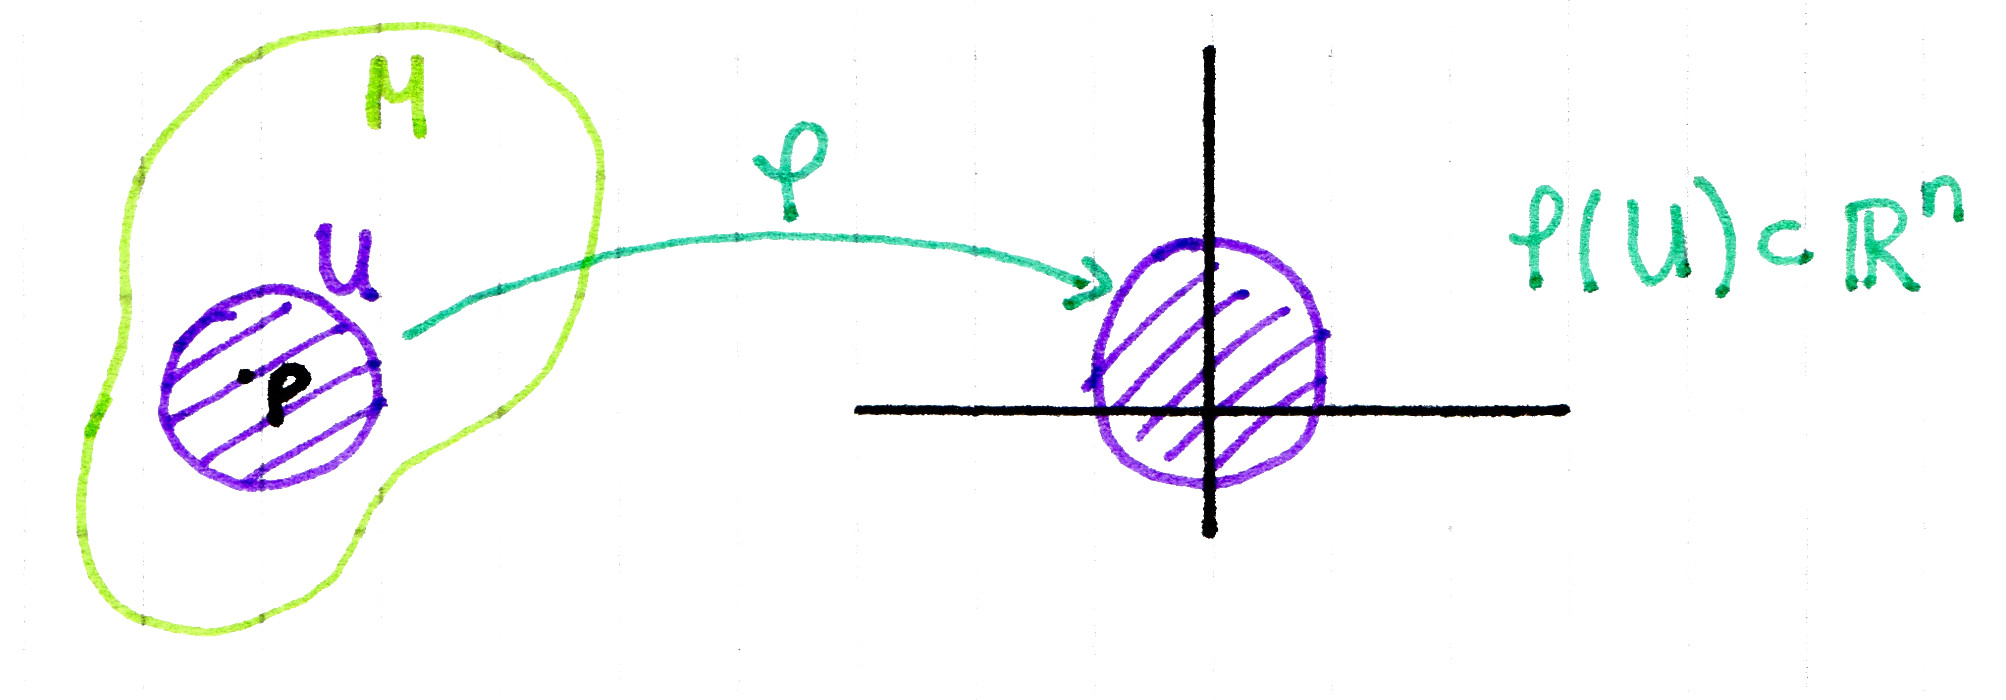
\includegraphics[width=.5\textwidth]{Karte}
      \caption{Karte von \( U \) mittels \( \phi \)}
    \end{figure}
    \item \( M \) ist \hyperref[def:hausdorffsch]{hausdorffsch} und besitzt abzählbare Basis der Topologie.
  \end{enumerate}
  \emph{Bemerkung}:
  \begin{itemize}
    \item Die zweite Eigenschaft ist ``technisch'' und garantiert, dass eine ``Zerlegung der Eins'' existiert (braucht man z.B. für die Existenz von Riemannschen Metriken). 
    \item Die Zahl \( n \) heißt \term{Dimension}\label{def:dimension} von \( M \) (eindeutig, wenn \( M \) \hyperref[def:zusammenhaengend]{zusammenhängend} ist, siehe \hyperref[th:satzGebietstreue]{Satz von Gebietstreue}). 
  \end{itemize}
\end{definition}

\begin{example}[{{\hyperref[def:topologischeMannigfaltigkeit]{Topologische Mannigfaltigkeiten}}}]
  \
  \begin{enumerate}
    \setcounter{enumi}{-1}

    \item Eine abzählbare Menge mit \hyperref[bsp:diskreteTopologie]{diskreter Topologie} (jeder Punkt ist offen) ist eine \( 0 \)-dimensionale Mannigfaltigkeit.

    \item \( S^1 \) ist eine \hyperref[def:kompakt]{kompakte}, \hyperref[def:zusammenhaengend]{zusammenhängenge} \( 1 \)-dimensionale Mannigfaltigkeit. \\
      \( \R \) ist nichtkompakte, zusammenhängende \( 1 \)-Mannigfaltigkeit.

    \begin{figure}[H]
      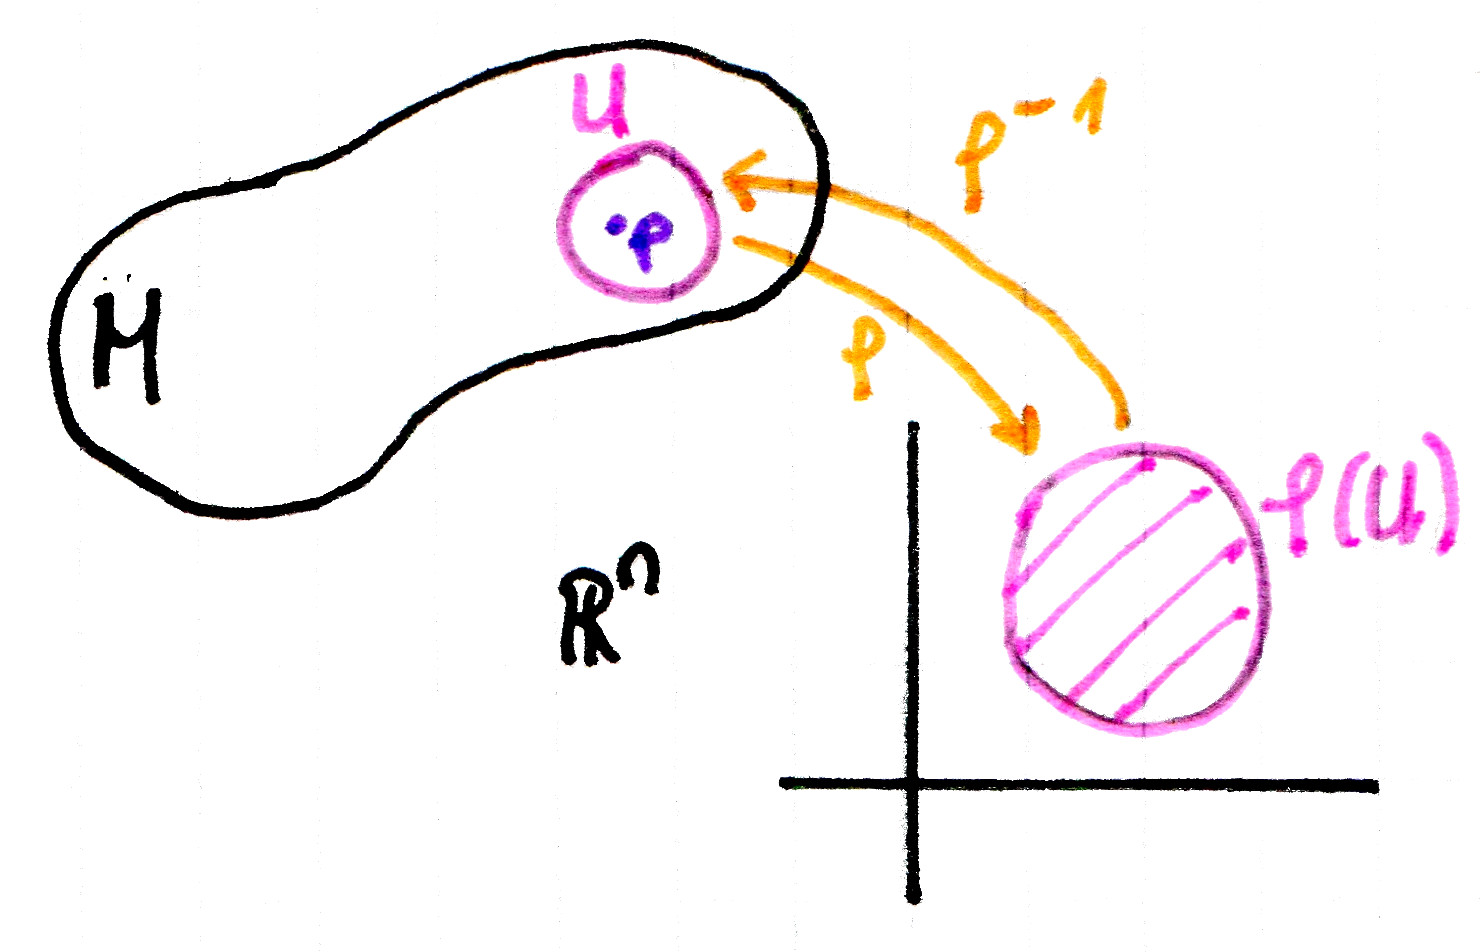
\includegraphics[width=.5\textwidth]{CharakteristikaMannigfaltigkeit}
      \captionsetup{width=.5\textwidth}
      \caption{Darstellung von \( \R \) und \( S^1 \) mit den für die topologische Mannigfaltigkeit nötigen Charakteristika}
    \end{figure}

    \item Jede offene Teilmenge einer Mannigfaltigkeit ist wieder eine Mannigfaltigkeit, z.B. ist jede offene Teilmenge von \( \R^n \) eine \( n \)-dimensionale Mannigfaltigkeit (hier ist \hyperref[def:karte]{Karte} = Einschränkung der Identität). \\
    \emph{Spezialfall}: \( \text{GL}(n,\R) = \{ A \in \R^{n \times n} : \det A \neq 0 \} \) ist offene Teilmenge von \( \R^{n^2} \), also eine \( n^2 \)-dimensionale Mannigfaltigkeit, denn:
    \begin{itemize}
      \item \( \det : \R^{n \times n} \to \R \) ist stetig
      \item \( \{ 0 \} \) ist abgeschlossen in \( \R \)
      \item \( \det^{-1} \{ 0 \} \) ist abgeschlossen in \( \R^{n \times n} \)
      \item \( \R^{n \times n} \setminus \det^{-1} \{ 0 \} = \text{GL}(n,\R ) \) ist offen in \( \R^{n \times n} \)
    \end{itemize}

    \begin{minipage}{.45\textwidth}
      \item Die \hyperref[bsp:einheitssphaere]{\( n \)-dimensionale Sphäre} mit Radius \( R > 0 \),
      \begin{equation*}
        S^n_R = \{ x \in \R^{n+1} : \Vert x \Vert = R \}\text{,}
      \end{equation*}
      ist \( n \)-dimensionale topologische Mannigfaltigkeit.
    \end{minipage}
    \hfill
    \begin{minipage}{.45\textwidth}
      \begin{figure}[H]
        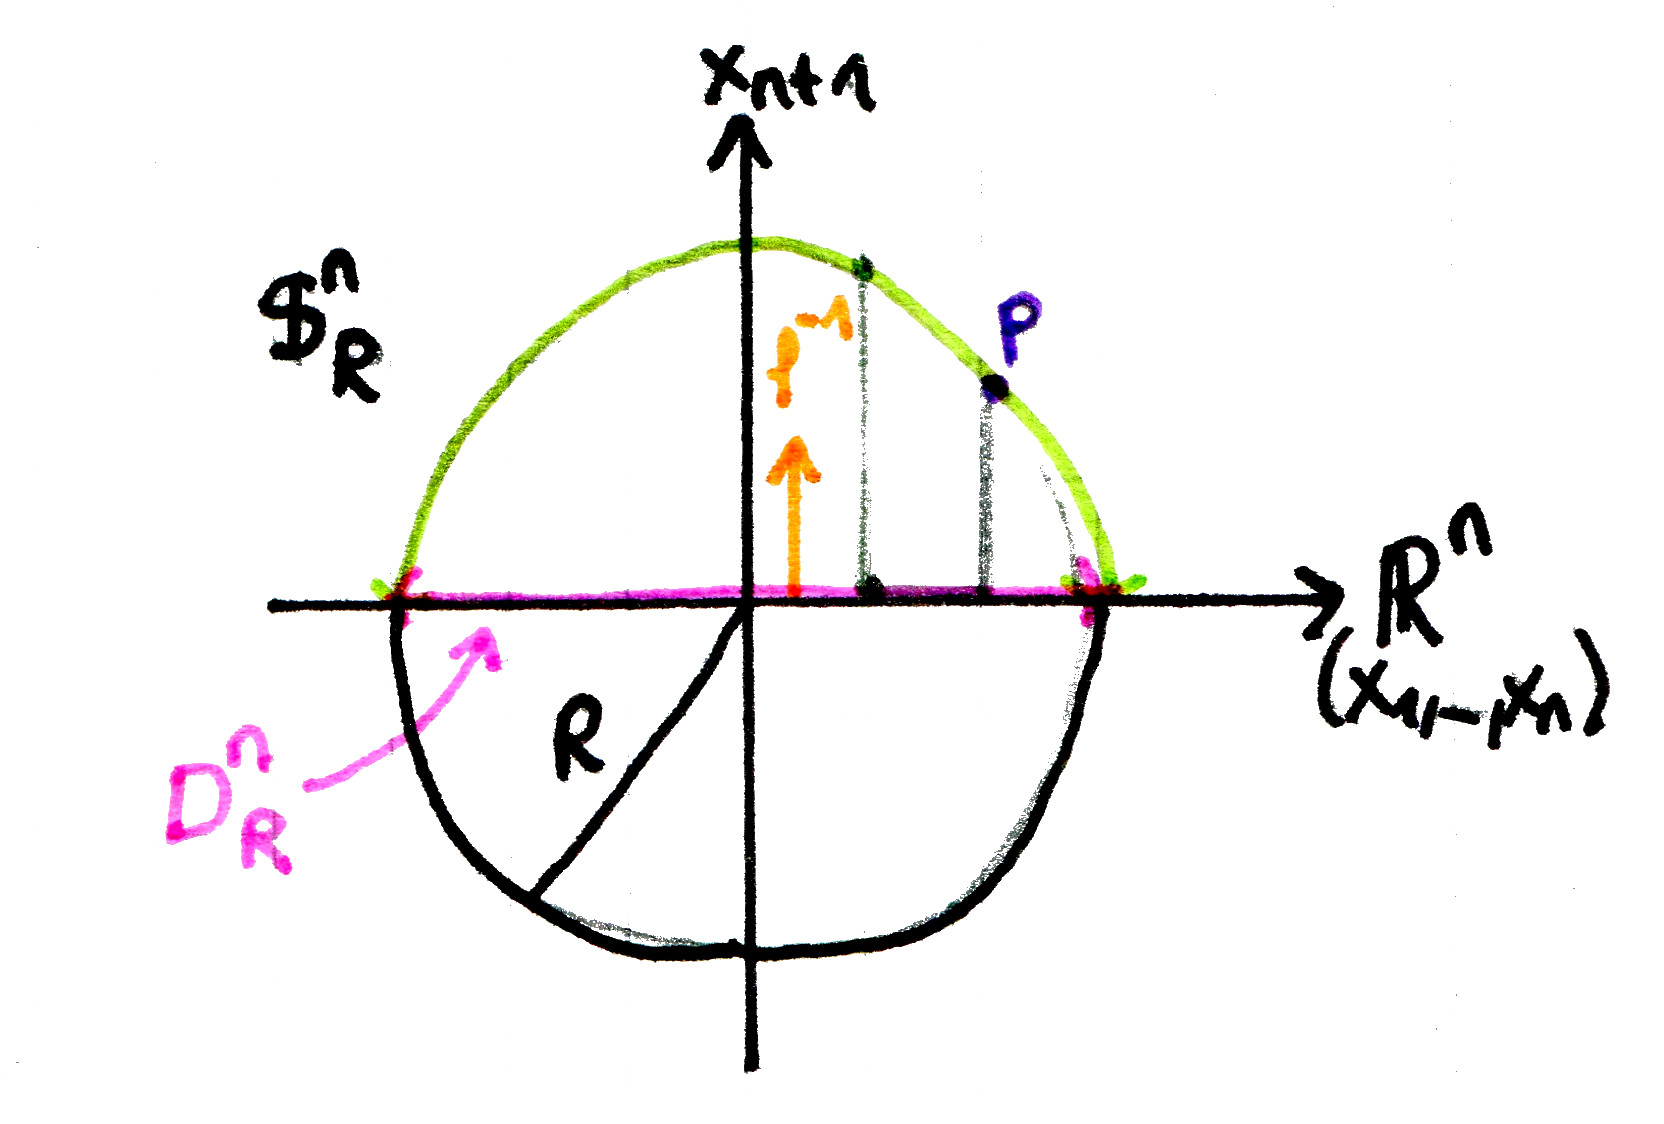
\includegraphics[width=.8\textwidth]{SphaereMannigfaltigkeit}
        \caption{\( n \)-dimensionale Sphäre als topologische Mannigfaltigkeit}
      \end{figure}
    \end{minipage}
    \begin{proof}
      Sei \( (x_1, \dots, x_{n+1}) = p \in S^n_R \), oBdA \( x_{n+1} > 0 \). Man betrachte die Abbildung
      \begin{align*}
        \phi^{-1} : D^n_R \coloneqq \left \{ x \in \R^n : \Vert x \Vert < R \right \} &\to \phi(D^n_R) \subset S^n_R \\
          (x_1, \dots, x_n) &\mapsto \left(x_1, \dots, x_n, \sqrt{R^2-(x_1^2 + \cdots + x_n^2)}\right)
      \end{align*}
      d.h. \( \phi \) ist Einschränkung der Orthogonalprojektion
      \begin{align*}
        \R^{n+1} &\to \R^n \subset \R^{n+1} \\
          (x_1, \dots, x_{n+1}) &\mapsto (x_1, \dots, x_n, 0)
      \end{align*}
      auf \( S_R^n \).
      \begin{figure}[H]
        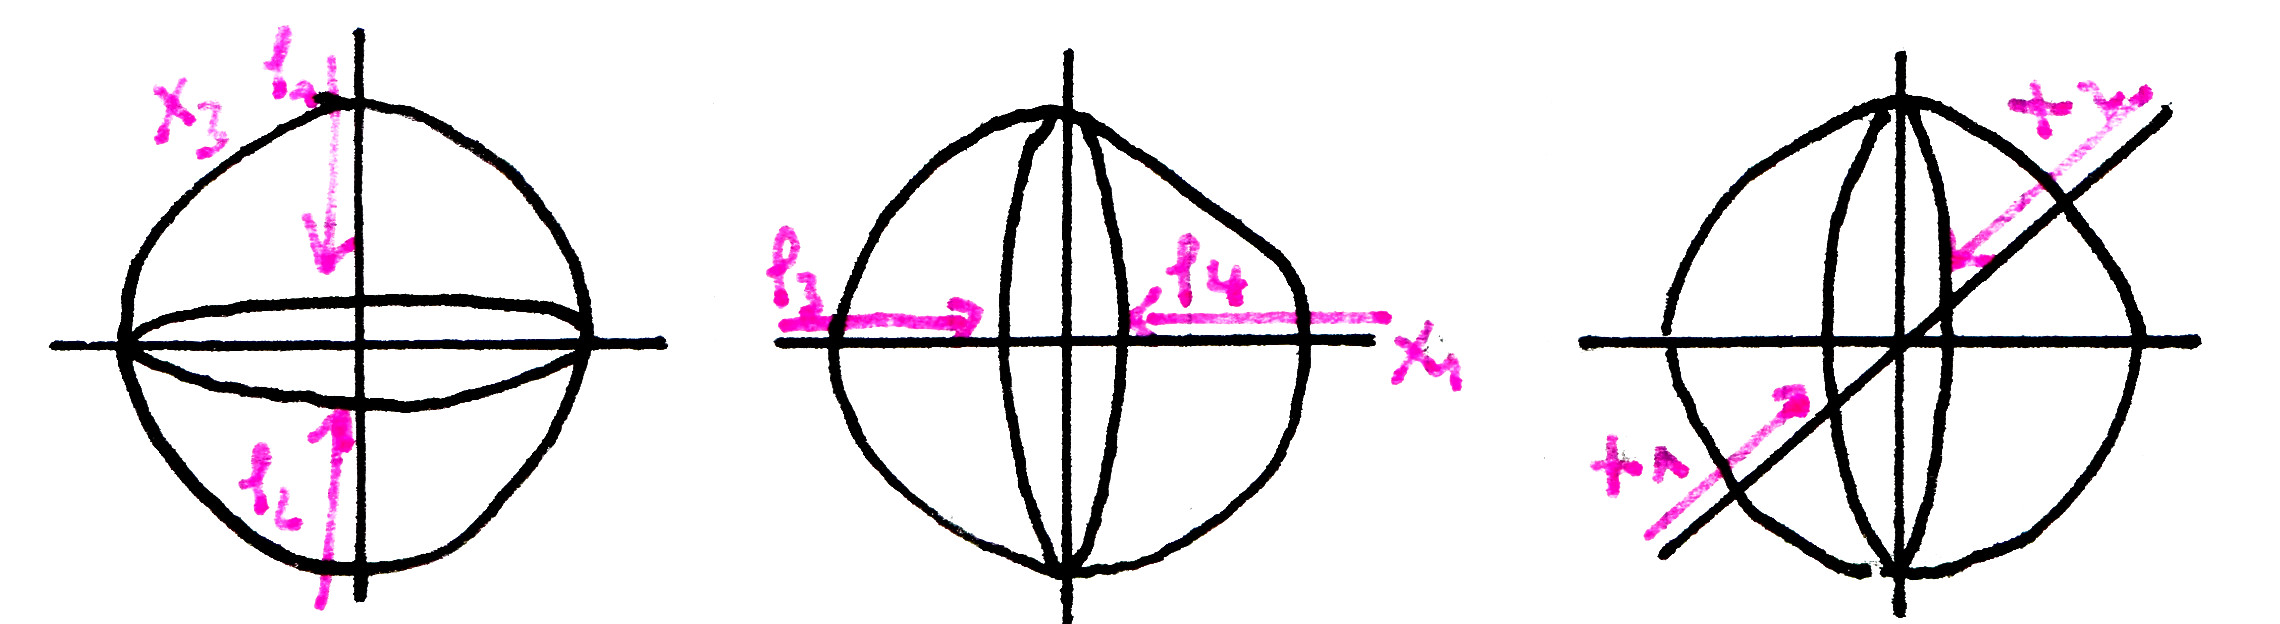
\includegraphics[width=.5\textwidth]{Orthogonalprojektion}
        \caption{Einschränkung der Orthogonalprojektion}
      \end{figure}
      Alternativ kann via stereographischer Projektion mit \( 2 \) Karten ausgekommen werden. \\
      Ein \hyperref[def:atlas]{Atlas} mit einer Karte existiert nicht. \qed{}
    \end{proof}
    \item Das Produkt von \( n_1 \)-dimensionaler Mannigfaltigkeit \( M_1 \) und \( n_2 \)-dimensionaler Mannigfaltigkeit \( M_2 \) ist \( (n_1+n_2) \)-dimensionale Mannigfaltigkeit. \\
    \emph{Karten}: \( (p_1, p_2) \in M_1 \times M_2 \),
    \begin{equation*}
      \widetilde{\phi} : U_1 \times U_2 \to \phi_1(U_1) \times \phi_2(U_2) \subset \R^{n_1} \times \R^{n_2}
    \end{equation*}
    mit \( (U_1, \phi_1) \) Karte von \( M_1 \) um \( p_1 \) und \( (U_2, \phi_2) \) Karte von \( M_2 \) um \( p_2 \).
  \end{enumerate}
\end{example}

\begin{remark}[``Wieviele {\hyperref[def:topologischeMannigfaltigkeit]{topologische Mannigfaltigkeiten}} gibt es?'']
  \
  \begin{itemize}
    \item \emph{Dimension} \( n=1 \): Im wesentlichen \( \R \) (nicht \hyperref[def:kompakt]{kompakt}) oder \( S^1 \) (kompakt).
    \item \emph{Dimension} \( n=2 \): Liste für \hyperref[def:zusammenhaengend]{zusammenhängende}, kompakte, ``orientierbare'', ``randlose'' Mannigfaltigkeiten:
    \begin{itemize}
      \item \( g = 0 \): \( S^2 \) \hyperref[bsp:einheitssphaere]{Einheitssphäre}
      \item \( g = 1 \): \( T^2 = S^1 \times S^1 \) Torus
      \item \( g = 2 \): Brezel
      \item \dots 
    \end{itemize}
    \( g \) ist das \term{Geschlecht}\label{def:geschlecht} der Mannigfaltigkeit.
    \item \emph{Dimension} \( n=3 \): Thurston's \term{Geometrisierungs-Vermutung}\label{theorem:geometrisierungsvermutung} (\( \sim \) 1978) \\
      Bewiesen von Perelman (2002), ein Milleniumsproblem.
    \item \emph{Dimension} \( n \geq 4 \): Allgemeine Klassifikation unmöglich, weil das Homöomorphieproblem hier nicht entscheidbar ist (Markov, 1960).
  \end{itemize}
\end{remark}

\section{Differenzierbare Mannigfaltigkeiten}

\begin{definition}[Kartenwechsel, differenzierbare Mannigfaltigkeit]
  \  \\

  \begin{minipage}{.45\textwidth}
    Sei \( M \) \hyperref[def:topologischeMannigfaltigkeit]{topologische Mannigfaltigkeit}, \( p \in M \). Ein \term{Kartenwechsel}\label{def:kartenwechsel} ist ein \hyperref[def:homoeomorphismus]{Homöomorphismus}
    \begin{equation*}
      \psi \circ \phi^{-1}: \underbrace{\phi(D)}_{\subset \R^n} \to \underbrace{\psi(D)}_{\subset \R^n}\text{.}
    \end{equation*}
  \end{minipage}
  \hfill
  \begin{minipage}{.45\textwidth}
    \begin{figure}[H]
      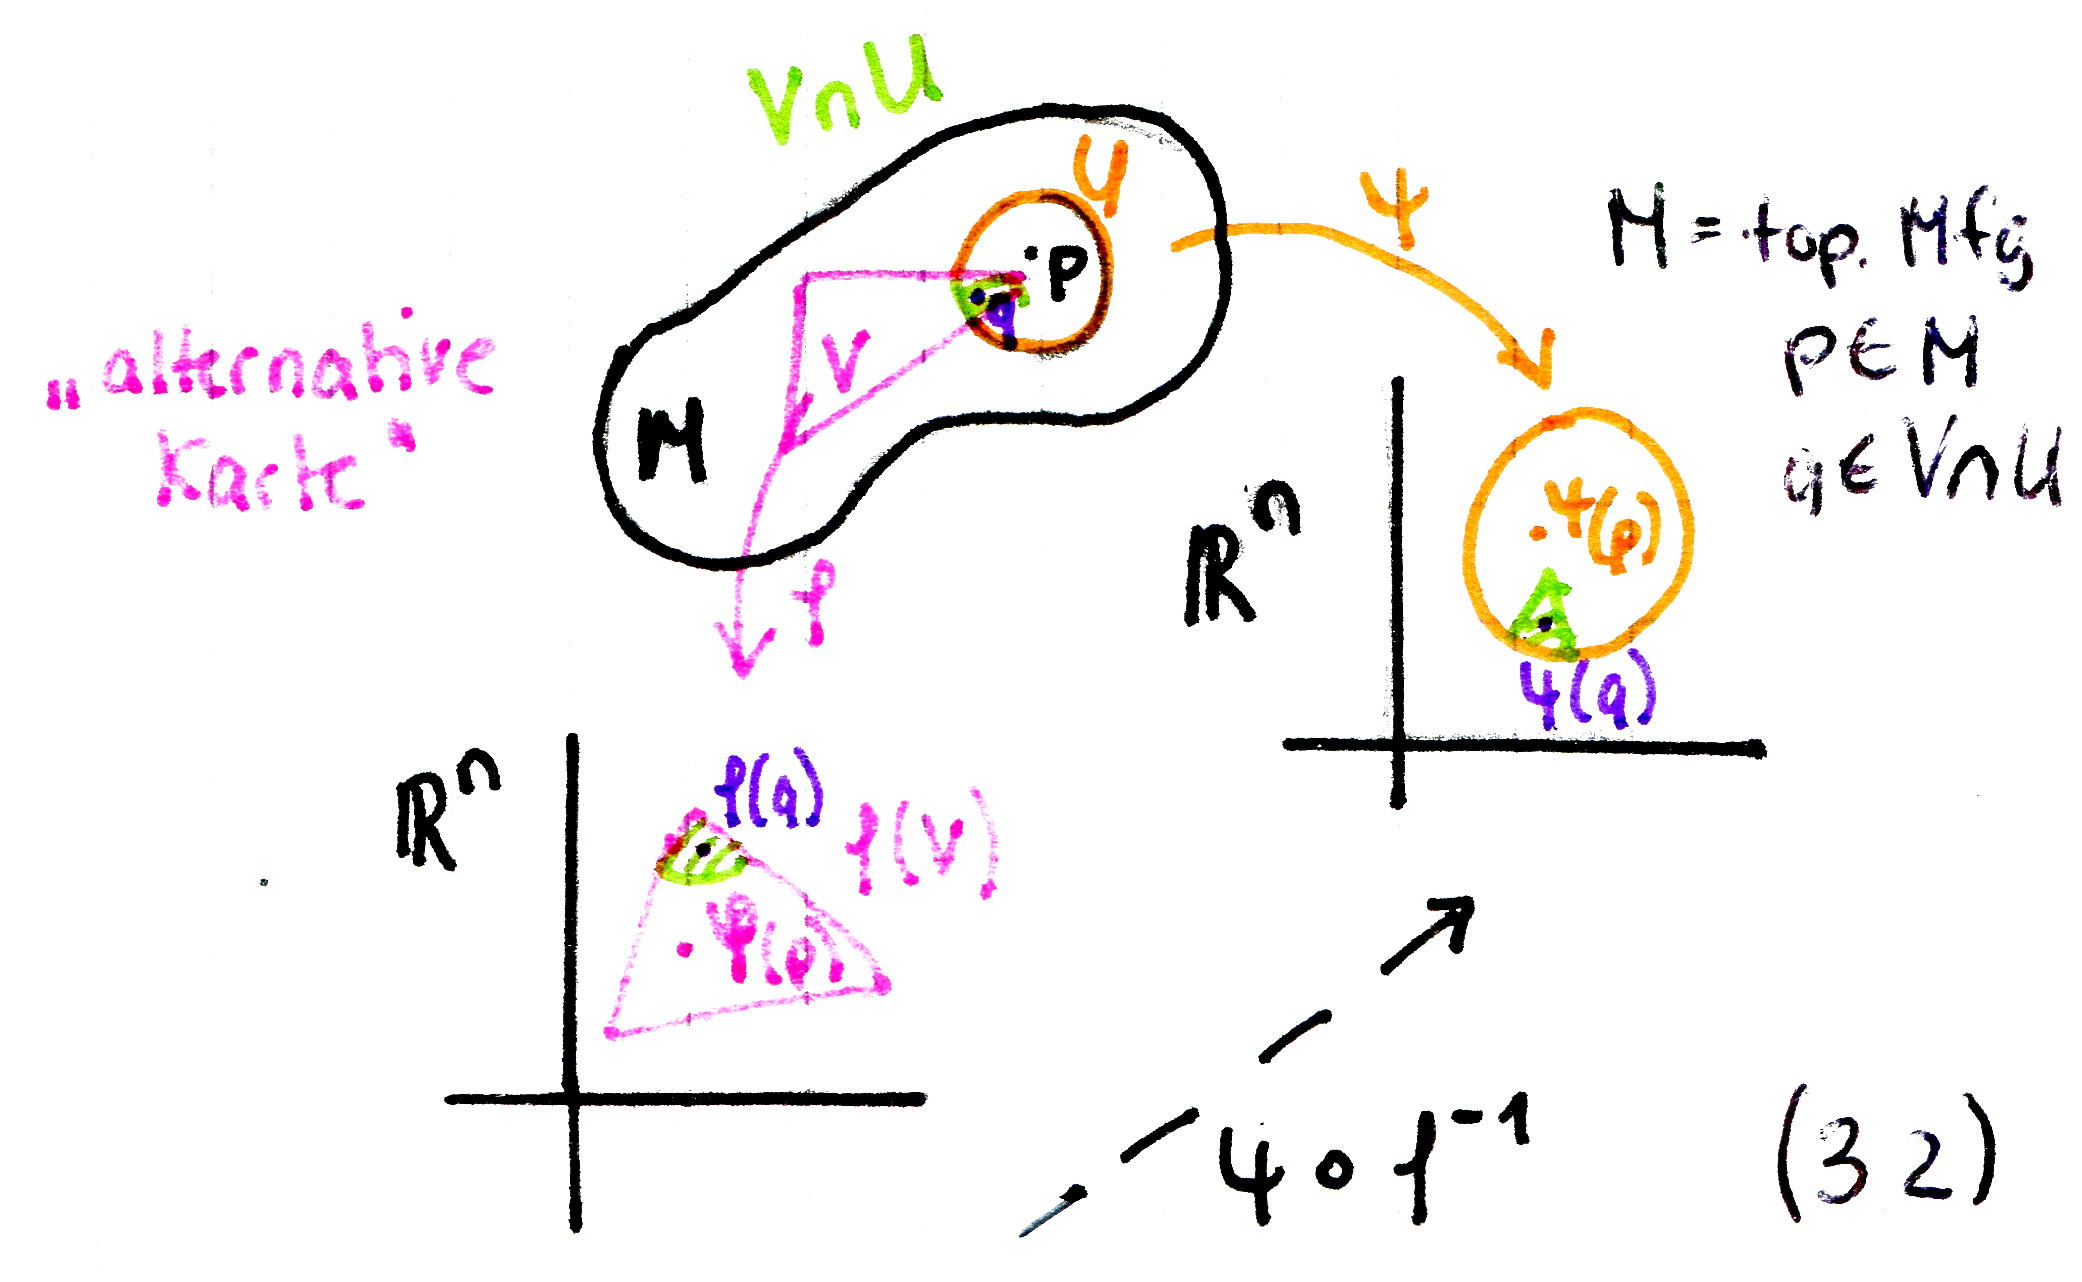
\includegraphics[width=\textwidth]{Kartenwechsel}
      \caption{Kartenwechsel}
    \end{figure}
  \end{minipage}
  Ein \hyperref[def:atlas]{Atlas} \( \mathcal{A} \) von \( M \) ist ein \term{\( C^\infty \)-Atlas}\label{def:dbatlas}, falls alle möglichen Kartenwechsel \( C^\infty \)-Abbildungen von \( \R^n \) sind, also alle partiellen Ableitungen existieren und stetig sind. \\
  Ein maximaler \( C^\infty \)-Atlas heißt \term{\( C^\infty \)-Struktur}\label{def:dbstruktur} auf der topologischen Mannigfaltigkeit \( M \). Eine \( C^\infty \)-Mannigfaltigkeit ist eine topologische Mannigfaltigkeit mit einer \( C^\infty \)-Struktur (auch \term{glatte}\label{def:glattemannigfaltigkeit} oder \term{differenzierbare Mannigfaltigkeit}\label{def:dbmannigfaltigkeit}).
\end{definition}

\begin{remark}
  \
  \begin{enumerate}
    \item Es gibt \hyperref[def:topologischeMannigfaltigkeit]{topologische Mannigfaltigkeiten} ohne \hyperref[def:dbstruktur]{differenzierbare Struktur}\footnote{Kerraire 1960}.
    \item Auf \( \R^n \), \( n \neq 4 \)\footnote{Kirby, Friedman 1980}, existiert genau eine differenzierbare Struktur.
    \item Auf \( S^7 \) existieren \( 28 \) differenzierbare Strukturen\footnote{Milnor 1956}.
  \end{enumerate}
  \emph{Frage}: Wozu das Differenzierbarkeitskriterium für \hyperref[def:kartenwechsel]{Kartenwechsel}? Beispielsweise für die Definition von differenzierbaren Abbildungen zwischen \hyperref[def:dbmannigfaltigkeit]{differenzierbaren Mannigfaltigkeiten}.
\end{remark}


\begin{definition}[Differenzierbarkeit]
  Seien \( M^m \), \( N^n \) \hyperref[def:dbmannigfaltigkeit]{differenzierbare Mannigfaltigkeiten} und \( F: M^m \to N^n \) stetig. \( F \) heißt \term{differenzierbar in \( p \in M \)}\label{def:differenzierbar}, falls für \hyperref[def:karte]{Karten} \( (U, \phi) \) um \( p \) und \( (V, \psi) \) um \( F(p) \) gilt:
  \begin{equation*}
    \psi \circ F \circ \phi^{-1}: \underbrace{\phi(U)}_{\subset \R^m} \to \underbrace{\psi(V)}_{\subset \R^n}
  \end{equation*}
  ist \( C^\infty \)-Abbildung in \( \phi(p) \). \\
  So kommt man von einem abstrakten \( F \) zwischen den Mannigfaltigkeiten zu einer konkreten Darstellung von \( F \). \\
  \( F \) heißt \term{differenzierbar} (\( C^\infty \)), falls \( F \) differenzierbar ist für alle \( p \in M \).
  \begin{figure}[H]
    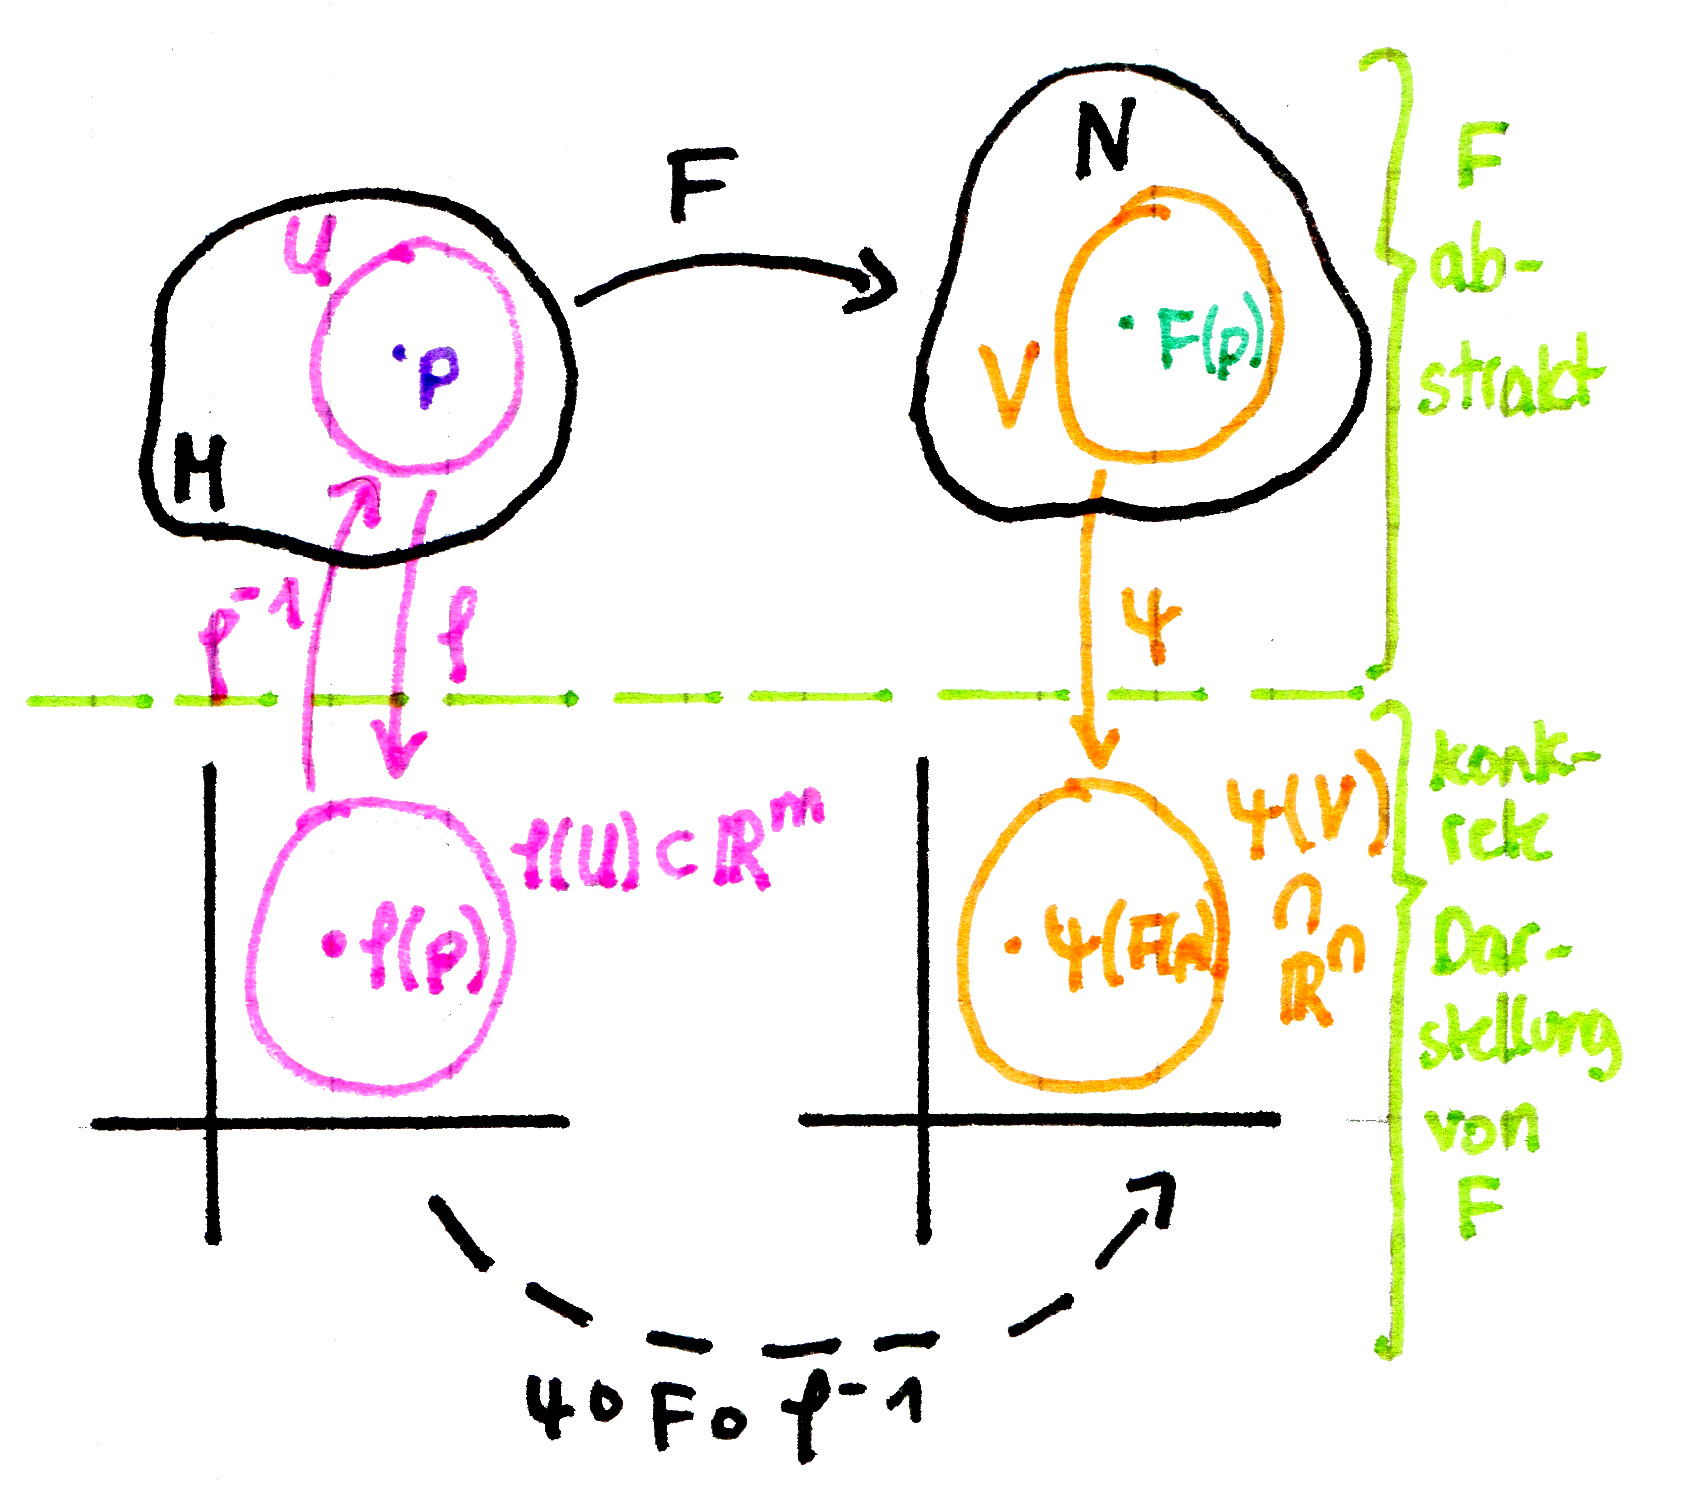
\includegraphics[width=.5\textwidth]{Differenzierbarkeitskriterium}
    \caption{Differenzierbarkeitskriterium}
  \end{figure}
\end{definition}

\begin{remark}[Wohldefiniertheit der Differenzierbarkeit]
  Differenzierbarkeit in \( p \) ist wohldefiniert (also unabhängig von der Wahl der Karten)
  \begin{proof}
    \emph{Erster Test}: \( \psi \circ F \circ \phi^{-1} \), \emph{zweiter Test} \( \widetilde{\psi} \circ F \circ \widetilde{\phi}^{-1} \) \\
    Es gilt:
    \begin{align*}
      \psi \circ F \circ \phi^{-1} &= \psi \circ \underbrace{\widetilde{\psi}^{-1} \circ \widetilde{\psi}}_{\text{Id}_{\R^n}} \circ F \circ \underbrace{\widetilde{\phi}^{-1} \circ \widetilde{\phi}}_{\text{Id}_{\R^n}} \circ \phi^{-1} \\
        &= \underbrace{\left( \psi \circ \widetilde{\psi}^{-1} \right)}_{C^\infty} \circ \left( \widetilde{\psi} \circ F \circ \widetilde{\phi}^{-1} \right) \circ \underbrace{\left( \widetilde{\phi} \circ \phi^{-1} \right)}_{\text{Kartenwechsel}}
    \end{align*}
    Also: Abbildung in Test 1 ist \( C^\infty \Leftrightarrow \) Abbildung in Test 2 ist \( C^\infty \). \qed{}
  \end{proof}
\end{remark}

\begin{remark}
  \
  \begin{itemize}
    \item \( N = \R \), \( F:M \to \R \) (differenzierbar) heißt \term{differenzierbare Funktion}.
    \item \( M = \R \) (oder \( I \subset \R \)), \( F: I \to N \) heißt \term{differenzierbare Kuve}.
    \item Eine Abbildung \( F: M \to N \) zwischen differenzierbaren Mannigfaltigkeiten heißt \term{Diffeomorphismus}\label{def:diffeomorphismus}, falls \( F \) bijektiv und \( F \) und \( F^{-1} \) differenzierbar sind (also \( C^\infty \)).
    \item Ein Homöomorphismus ist nicht unbedingt ein Diffeomorphismus. Beispielsweise \( \R \) mit Id als Karte, \( F : \R \to \R \), \( x \mapsto x^3 \) ist Homöomorphismus, aber kein Diffeomorphismus, da \( F^{-1} : x \mapsto \sqrt[3]{x} \) ist nicht \( C^\infty \).
    \item Die Menge der Diffeomorphismen einer differenzierbaren Mannigfaltigkeit ist eine Gruppe mit der Verkettung von Abbildungen.
  \end{itemize}
\end{remark}

\begin{example}
  \
  \begin{enumerate}
    \item \( U \subseteq \R^n \) offen (bzgl. Standard-Topologie). \\
      \( \phi_0 \coloneqq \text{Id}\mid_U \) mit zugehörigem maximalen Atlas definiert \( C^\infty \)-Struktur auf \( U \), die kanonische differenzierbare Struktur.
    \item \( 2 \)-dimensionale Mannigfaltigkeiten heißen auch \term{Flächen}\label{def:flaeche}, speziell \emph{regulär parametrisierte Flächen}\footnote{Gegenstand der klassischen Differentialgeometrie, siehe auch Kapitel 5}.
  \end{enumerate}
\end{example}

\begin{definition}[Reguläre Fläche]
  Eine Teilmenge \( S \) von \( \R^3 \) (mit Teilraum-Topologie von \( \R^3 \)) heißt \term{reguläre Fläche}\label{def:regulaereFlaeche}, falls für jeden Punkt \( p \in S \) eine Umgebung \( V \) von \( p \) in \( \R^3 \) und eine Abbildung
  \begin{align*}
    F : \underset{\text{offen}}{U} \subset \R^2 &\to \underset{\text{offene TM von S}}{V \cap S} \subset \R^3 \\
      (u,v) &\mapsto (x(u,v),y(u,v),z(u,v))
  \end{align*}
  existiert, so dass gilt:
  % TODO Abbildung 2
  \begin{enumerate}
    \item \( F \) ist ein differenzierbar Homöomorphismus
    \item das Differential (Jacobi-Matrix) von \( F \),
    \begin{equation*}
       \text{d}F_q : \R^2 \supseteq T_q U \to T_{F(q)}\R^3 \cong \R^3
     \end{equation*} 
     ist \emph{injektiv} (d.h. Jacobi-Matrix hat Rang \( 2 \)) für \( \forall q \in U \).
  \end{enumerate}
  \( F \) heißt \term{lokale Parametrisierung}\label{def:lokaleParametrisierung} von \( S \).
  \begin{figure}[H]
    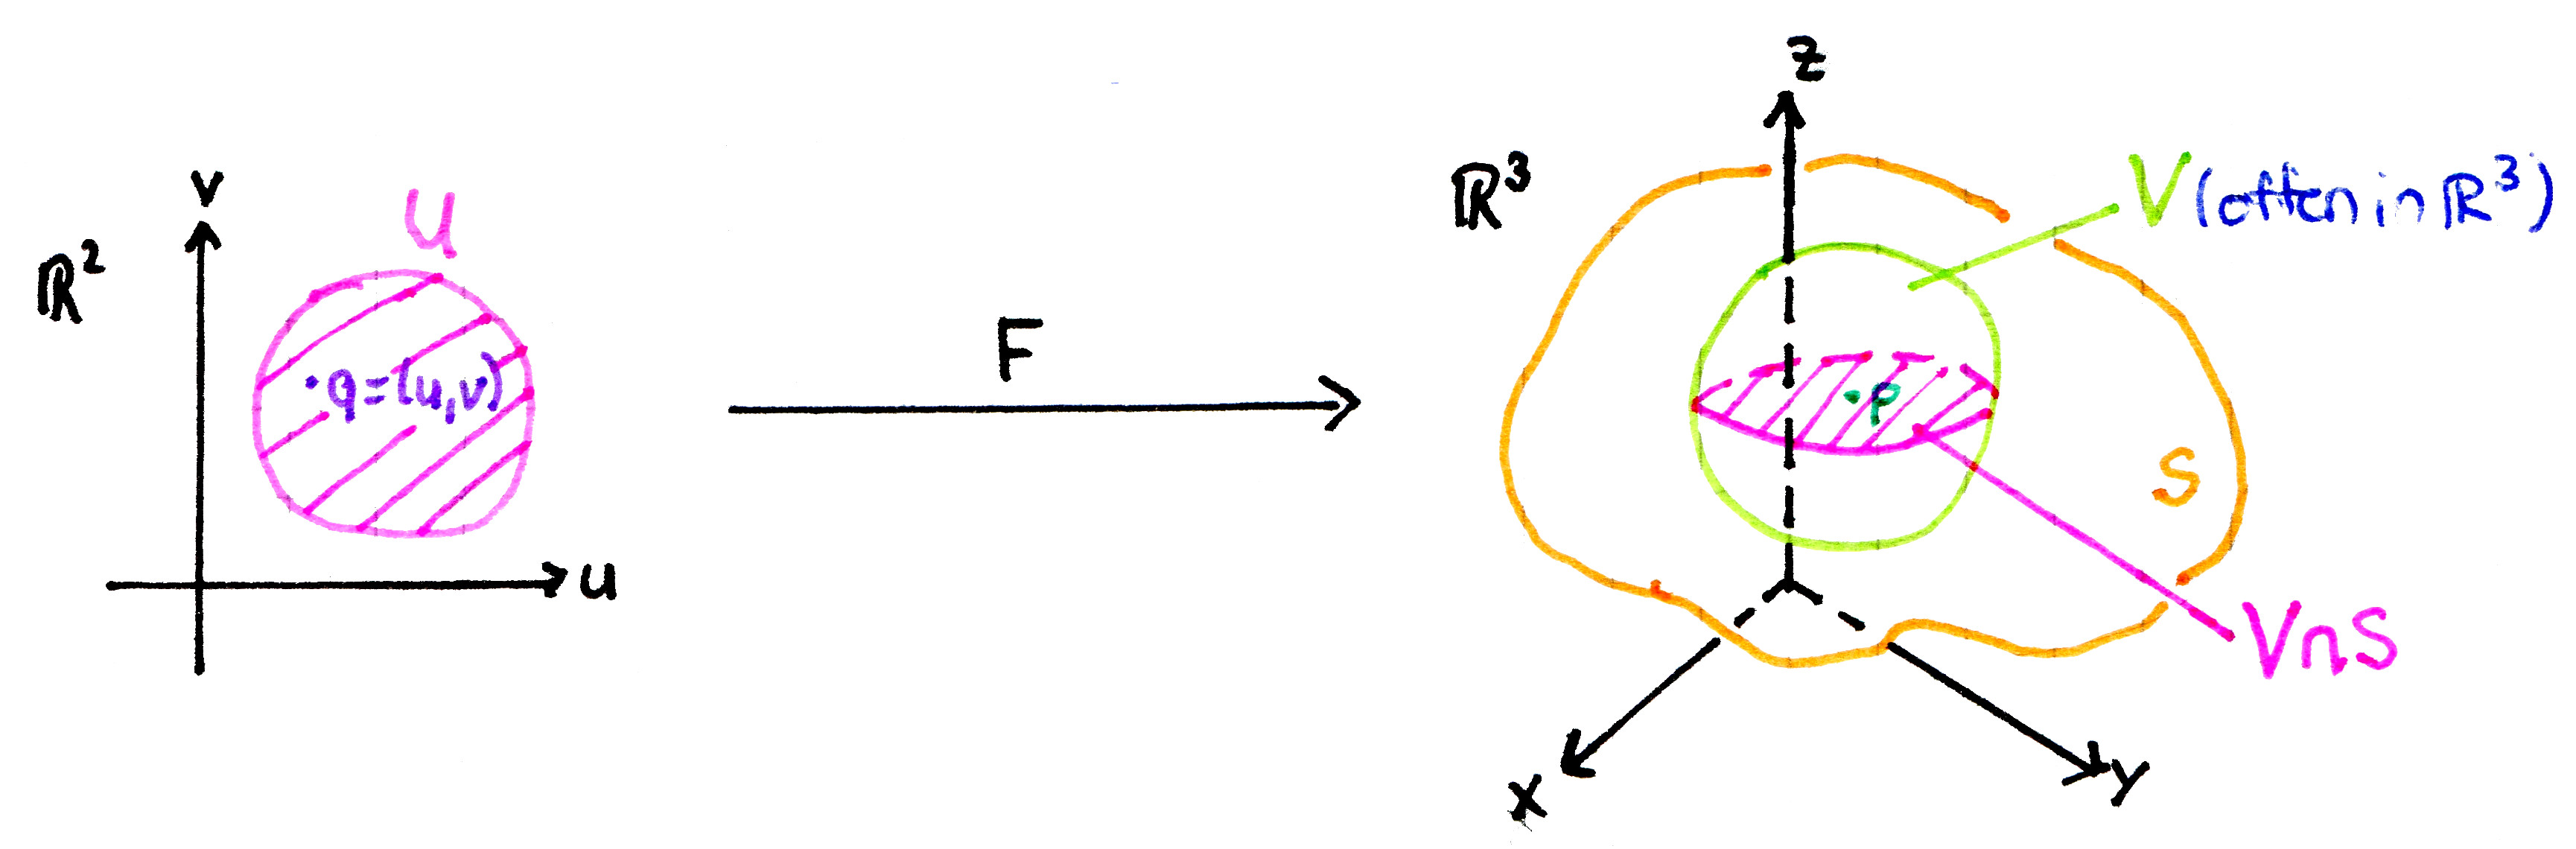
\includegraphics[width=.8\textwidth]{LokaleParametrisierung}
    \caption{Lokale Parametrisierung}
  \end{figure}
\end{definition}

\begin{example}[Rotationsfläche]
  Gegeben ist eine ebene Kurve \( c(v) = \left( r(v), 0, h(v) \right) \), \( v \in [a,b] \) mit \( r(v) > 0 \), \( c'(v) = \left( r'(v), 0, h'(v) \right) \) Tangentialvektor (mit \( C^\infty \)-Funktionen \( r \), \( h \)).\footnote{\( \Vert c'(v) \Vert \neq 0 \Leftrightarrow {(r')}^2 + {(h')}^2 \neq 0 \)}

  \begin{minipage}{.45\textwidth}
    \begin{equation*}
      F(u,v) \coloneqq \begin{pmatrix}
        r(v)\cos u \\
        r(v)\sin u \\
        h(v)
      \end{pmatrix}
    \end{equation*}
    ist reguläre Fläche.\footnotemark{} \\
    \emph{Beispiel}: \( 2 \)-Sphäre von Radius \( R \):
    \begin{equation*}
      (u,v) \mapsto \begin{pmatrix}
        R\cos v \cos u \\
        R\cos v\sin u \\
        R\sin v
      \end{pmatrix}\text{.}
    \end{equation*}
  \end{minipage}
  \footnotetext{Übung!}
  \hfill
  \begin{minipage}{.45\textwidth}
    \begin{figure}[H]
      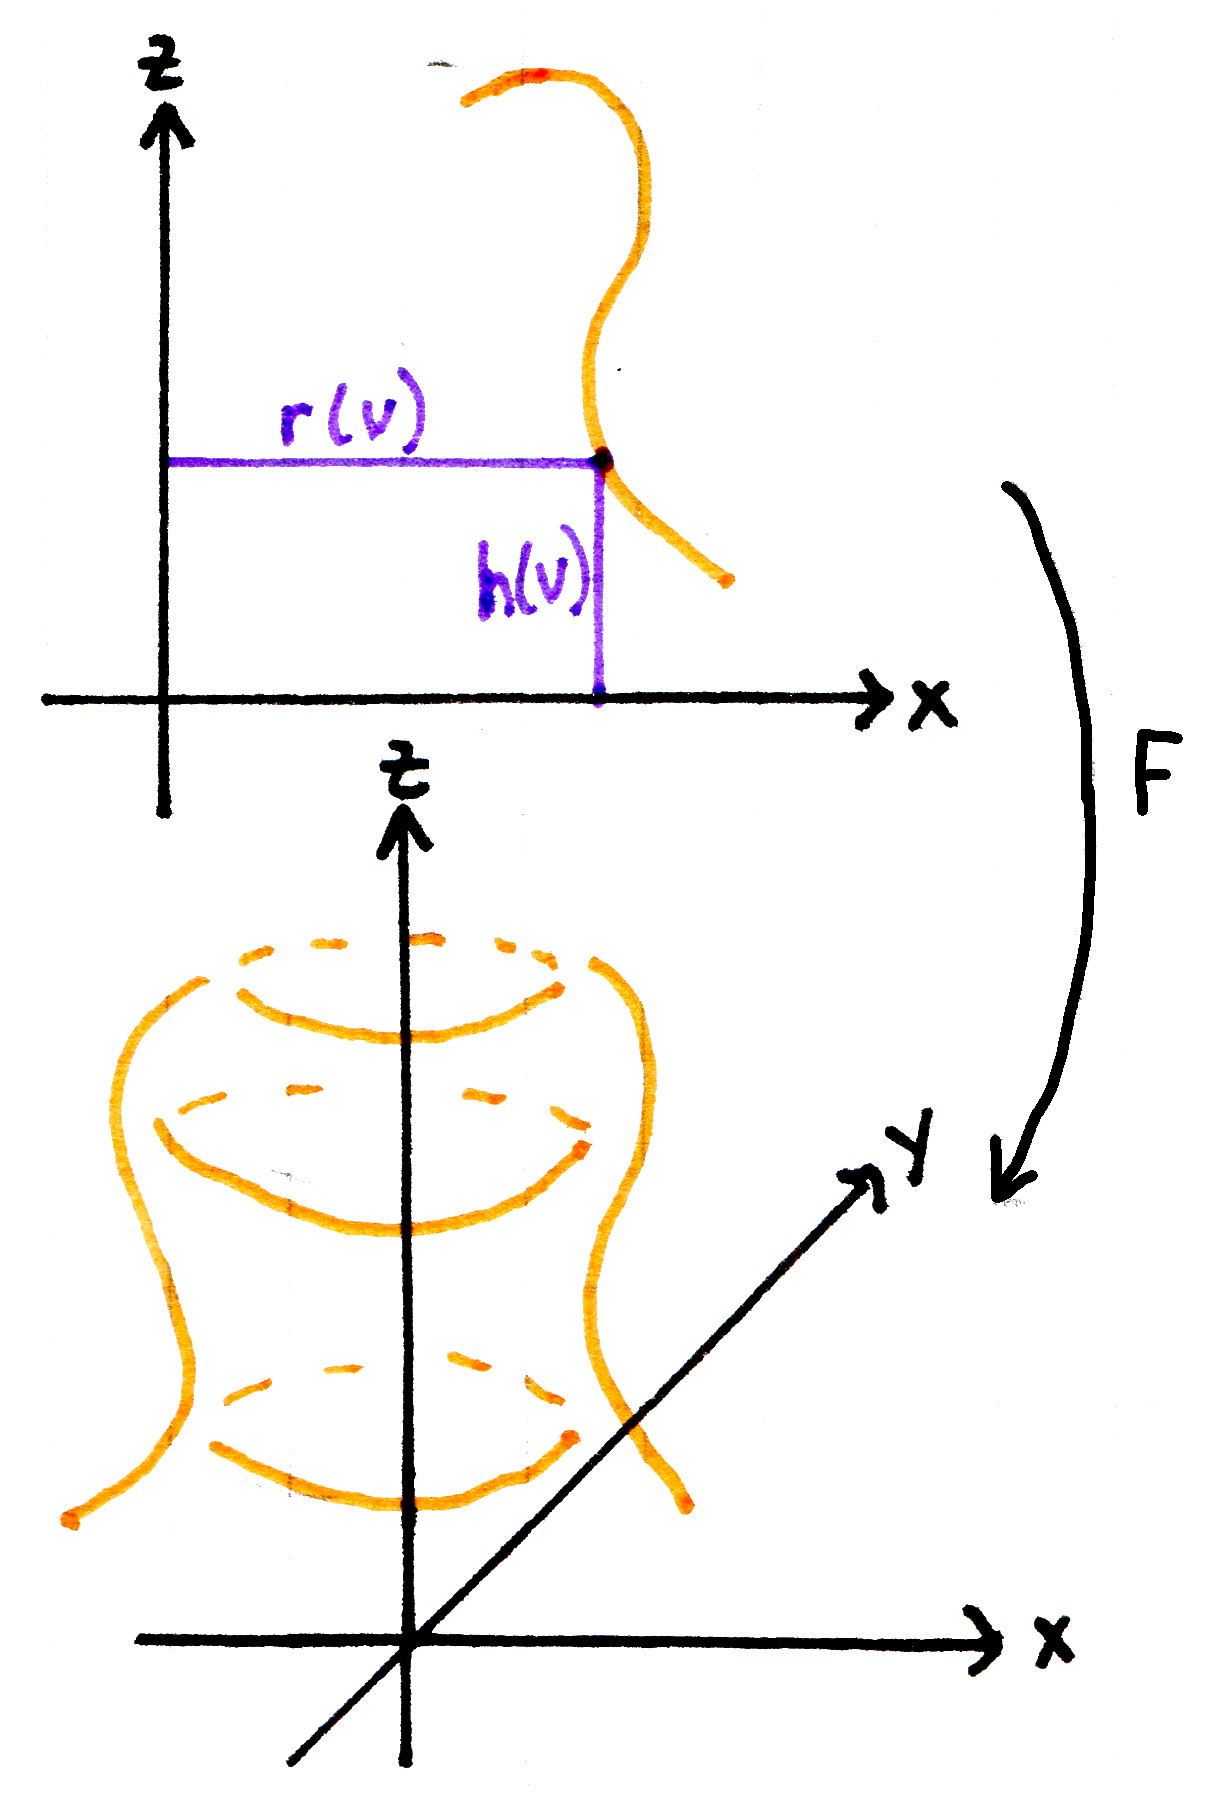
\includegraphics[width=.8\textwidth]{Rotationsflaeche}
      \caption{Rotationsfläche}
    \end{figure}
  \end{minipage}

  Es gibt andere Parametrisierungen, beispielsweise
  \begin{equation*}
    (u,v) \mapsto \begin{pmatrix}
      u \\ v \\ \sqrt{R^2-u^2-v^2}
    \end{pmatrix}
  \end{equation*}
  % TODO Abbildung 4
\end{example}

\begin{remark}[Geometrische Eigenschaften parametrisierungsunabhängig]
  \  \\
  Geometrische Eigenschaften sollten unabhängig sein von Parametrisierung. Das wird durch Eigenschaft 2 von regulären Flächen garantiert. Genauer gilt: Parameterwechsel sind differenzierbar (\( \leadsto \) reguläre Flächen sind differenzierbare \( 2 \)-dimensionale Mannigfaltigkeiten mit \( F^{-1} \) (Umkehr-Abbildung der Parametrisierung) als Karten): \\
  Sei \( p \in S \) und \( F_1 : \R^2 \supseteq U \to S \), \( F_2: \R^2 \supseteq V \to S \) zwei Parametrisierungen, sodass \( p \in F_1(U) \cap F_2(V) \eqqcolon W \). \\
  \emph{Behauptung}: Der Parameterwechsel 
  \begin{equation*}
    H \coloneqq F_1^{-1} \circ F_2 : \R^2 \supset F_2^{-1}(W) \to F_1^{-1}(W) \subset \R^2
  \end{equation*}
  ist Diffeomorphismus.
  \begin{figure}[H]
    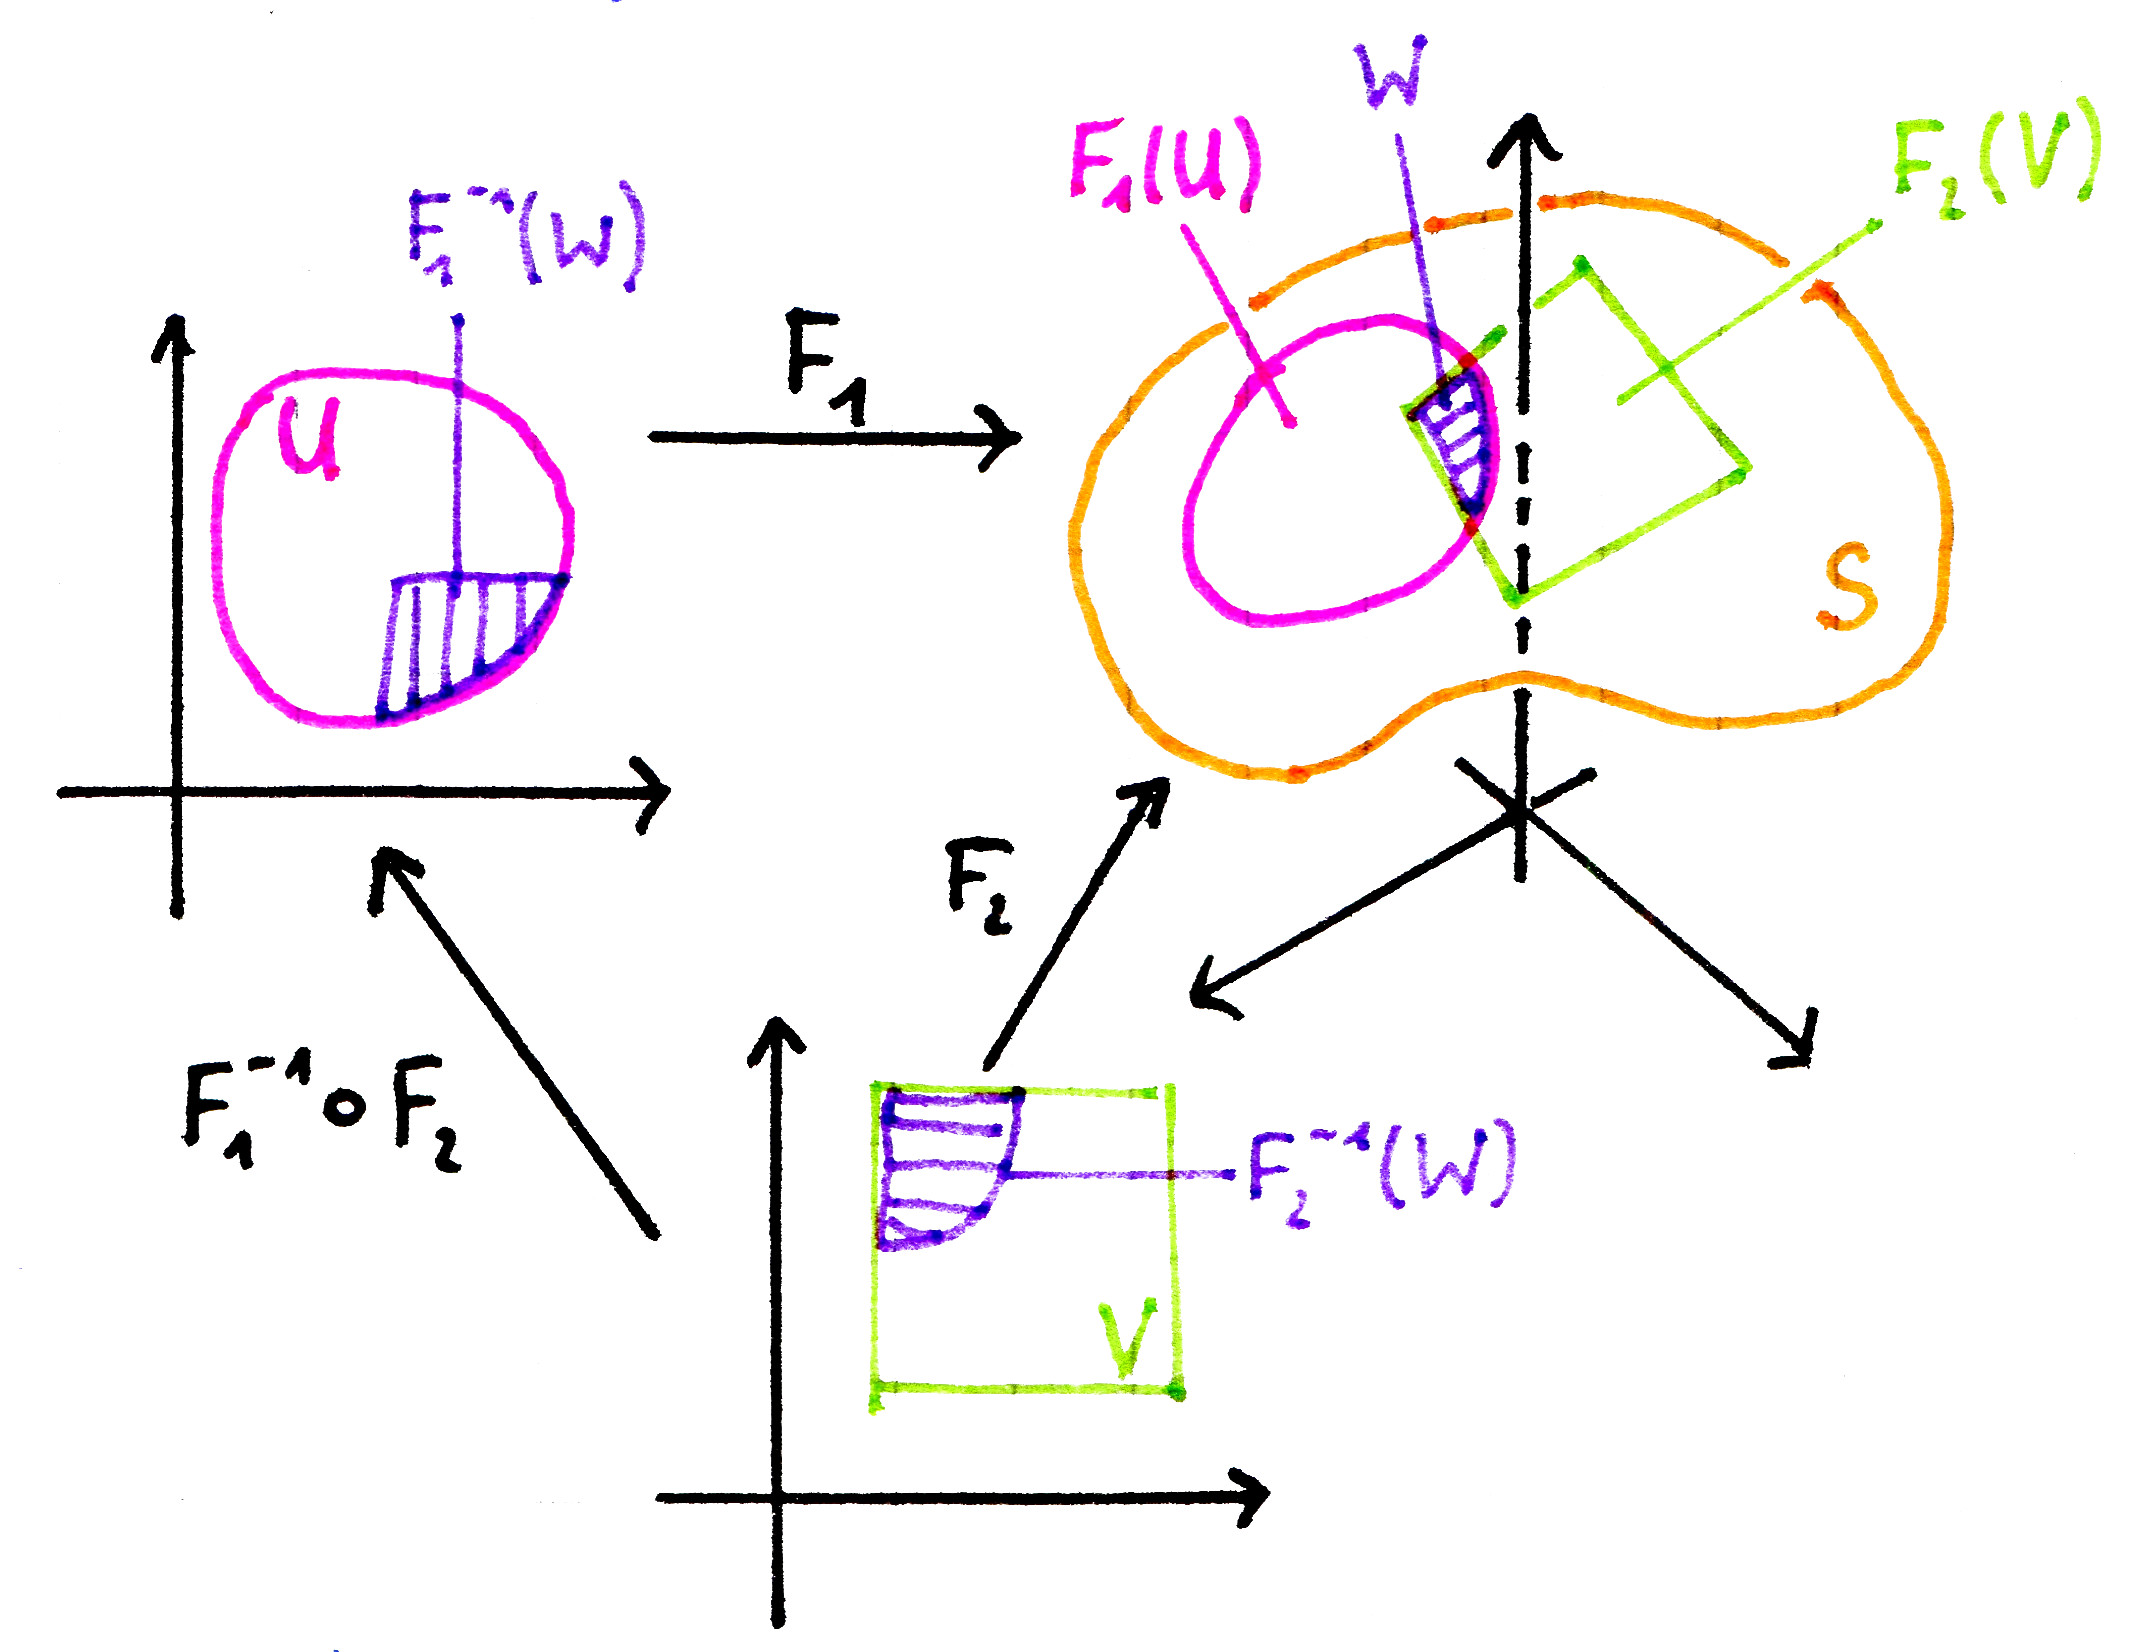
\includegraphics[width=.5\textwidth]{Parameterwechsel}
    \caption{Parameterwechsel}
  \end{figure}
  \begin{proof}
    \( H \) ist Homöomorphismus, da \( F_1 \) und \( F_2 \) Homöomorphismen sind. \\
    \emph{Problem}: \( F_1^{-1} \) ist auf einer offenen Teilmenge von \( S \) definiert und und da weiß man nicht was \emph{differenzierbar} heißt. \\
    \emph{Ausweg}: Erweiterung von \( F \). Sei \( r \in F_2^{-1}(W) \) und \( q \coloneqq H(r) \). Da
      \begin{equation*}
        F_1(u,v) = \left( x(u,v),y(u,v),z(u,v) \right)
      \end{equation*}
    reguläre Parametrisierung ist können wir oBdA (erst Koordinatenachsen von \( \R^3 \) umbenennen) annehmen, dass
    \begin{equation*}
      \frac{J(x,y)}{J(u,v)}(q) \neq 0 \quad \text{(Jacobi-Determinante).}
    \end{equation*}
    \emph{Trick}: Erweitere \( F_1 \) zu Abbildung
    \begin{align*}
      \widetilde{F_1} : U \times \R &\to \R^3 \\
        \widetilde{F_1}(u,v,t) &\coloneqq \left( x(u,v),y(u,v),z(u,v)+\bm{t} \right)\text{.}
    \end{align*}
    \( \widetilde{F_1} \) ist differenzierbar und \( \widetilde{F_1}|_{U \times \{ 0 \}} = F_1 \). \\
    Die Jacobi-Determinante von \( \widetilde{F_1} \) in \( (q,0) \),
    \begin{equation*}
      \det \begin{pmatrix}
        \frac{\text{d}x}{\text{d}u} & \frac{\text{d}x}{\text{d}v} & 0 \\
        \frac{\text{d}y}{\text{d}u} & \frac{\text{d}y}{\text{d}v} & 0 \\
        \frac{\text{d}z}{\text{d}u} & \frac{\text{d}z}{\text{d}v} & 1
      \end{pmatrix}(q,0) = \det \begin{pmatrix}
        \frac{\text{d}x}{\text{d}u} & \frac{\text{d}x}{\text{d}v} \\
        \frac{\text{d}y}{\text{d}u} & \frac{\text{d}y}{\text{d}v}
      \end{pmatrix}(q) \neq 0\text{.}
    \end{equation*}
    Nach dem Umkehrsatz (Analysis II) existiert eine Umgebung \( A \) von \( \widetilde{F_1}(q,0) = F_1(q) \) in \( \R^3 \) sodass \( \widetilde{F_1}^{-1} \) auf \( A \) existiert und differenzierbar (\( C^\infty \)) ist. Da \( F_2 \) stetig ist existiert Umgebung \( B \) von \( v \) in \( V \), sodass \( F_2(B) \subset A \). Und nun ist \( H|_B = \widetilde{F_1}^{-1} \circ F_2|_B \) ist Verkettung von differenzierbaren Abbildungen, also differenzierbar in \( r \) und da \( r \) beliebig ist ist \( H \) differenzierbar auf \( F_2^{-1}(W) \). \qed{}
  \end{proof}
\end{remark}

\begin{example}[Weitere Beispiele von differenzierbaren Mannigfaltigkeiten]
  \
  \begin{enumerate}
    \item \textbf{n-Sphäre} von Radius \( R \) (und Zentrum \( 0 \)):
      \begin{equation*}
        S_R^n \coloneqq \{ x \in \R^{n+1} : \Vert x \Vert = R \}\text{.}
      \end{equation*}
      Karten via stereographischer Projektion.
      \begin{align*}
        &N \coloneqq (0, \dots, 0, R), \quad &S \coloneqq (0, \dots, 0, -R) \\
        &U_1 \coloneqq S_R^n \setminus \{ N \}, \quad &U_2 \coloneqq S_R^n \setminus \{ S \}
      \end{align*}
      Stereographische Projektion bzgl \( N \):
      \begin{equation*}
        \phi_1 : U_1 \to \R^n, \ p = (p_1, \dots, p_{n+1}) \mapsto \left( x_1(p), \dots, x_n(p) \right), \ x_i(p) \coloneqq \frac{Rp_i}{R-p_{i+1}}
      \end{equation*}
      Stereographische Projektion bzgl. \( S \):\footnote{\textbf{Übung}: \( \phi_1 \) und \( \phi_2 \) sind Homöomorphismen.}
      \begin{equation*}
        \phi_1 : U_2 \to \R^n, \ p = (p_1, \dots, p_{n+1}) \mapsto \left( x_1(p), \dots, x_n(p) \right), \ x_i(p) \coloneqq \frac{Rp_i}{R-p_{i+1}}
      \end{equation*}
      Kartenwechsel:
      \begin{equation*}
        \phi_2 \circ \phi_1^{-1} : \R^n \setminus \{ 0 \} \to \R^n \setminus \{ 0 \}, \ \phi_2 \circ \phi_1^{-1}(x) = \frac{x}{\Vert x \Vert}R^2
      \end{equation*}
      ist \( C^\infty \). \\
      \( \Rightarrow \mathcal{A} \coloneqq \{ (U_1, \phi_1), (U_2, \phi_2) \} \) ist ein differenzierbarer Atlas für \( S_R^n \). \\
      \( \leadsto \) maximaler Atlas aller mit \( \mathcal{A} \) verträglichen Karten (also allen \( (U, \phi) \) mit \( \phi \circ \psi^{-1} \) ist \( C^\infty \) für \( \psi \) aus \( \mathcal{A} \) sofern Verkettung definiert ist) definiert differenzierbare Struktur auf \( S_R^n \), also ist \( S_R^n \) eine \( C^\infty \)-Mannigfaltigkeit mit Dimension \( n \).
    \item \( n \)-dimensionaler reell projektiver Raum
      \begin{equation*}
        P^n\R \coloneqq \{ \text{1-dim. UVR von } \R^{n+1} \} \equiv \left( \R^{n+1} \setminus \{ 0 \} \right) /\sim
      \end{equation*}
      mit \( x \sim y \overset{\text{Def.}}{\Leftrightarrow} \ \exists \ \R \ni \lambda \neq 0 : x = \lambda y \) (\( 1 \)-dimensionaler UVR = Äquivalenzklasse) \( \equiv S^n/\sim \) mit \( x \sim y \overset{\text{Def.}}{\Leftrightarrow} x = -y \). \\
      Wir sehen: \\
      \emph{1. Definition}: Eindimensionale Untervektorräume \\
      \emph{2. Definition}: Äquivalenzklassen in \( \R^{n+1} \setminus \{ 0 \} \) \\
      \emph{3. Definition}: Äquivalenzklassen in \( S^n \) \\
      Es ist leicht zu sehen, dass diese Definitionen äquivalent sind. \\
      Aus der 3. Definition sieht man
      \begin{equation*}
        P^n\R = S^n/\sim
      \end{equation*}
      ist kompakt als Quotientenraum von \( S^n \) (Quotiententopologie \( X \overset{\pi}{\to} Y = X/\sim \) mit topologischem Raum \( X \) und Quotiententopologie: \( U \) offen in \( Y \Leftrightarrow \pi^{-1}(U) \) ist offen in \( X \)). Diese Abbildung ist stetig, und ein stetiges Bild von einer kompakten Menge ist wieder kompakt. \\
      \textbf{Karten}:
      \begin{align*}
        \tilde{U_i} &\coloneqq \{ x \in S^n : x_i \neq 0 \}, \quad i = 1, \dots, n+1 \\
        U_i &\coloneqq \pi(\tilde{U_i}) \text{ mit } \pi: S^n \to S^n/\sim = P^n\R\text{.}
      \end{align*}
      Projektion:
      \begin{equation*}
        \phi_i : U_i \to \R^n, \quad \phi_i([x]) \coloneqq \left( \frac{x_i}{x_i}, \dots, \frac{x_{i-1}}{i}, \frac{x_{i+1}}{i}, \dots, \frac{x_n}{x_i} \right)
      \end{equation*}
      sind Homöomorphismen.\footnote{\textbf{Übung}: Kartenwechsel \( \phi_i \circ \phi_j^{-1} \) sind \( C^\infty \).}
  \end{enumerate}
\end{example}

\begin{remark}
  Man kann zeigen: \( P^n\R \) ist hausdorffsch und hat eine abzählbare Basis der Topologie. Also ist \( P^n\R \) eine \( n \)-dimensionale \( C^\infty \)-Mannigfaltigkeit. \\
  \emph{Analog}: \( P^n\C \coloneqq \{ \text{komplexe \( 1 \)-dim. UVR von } C^{n+1} \} \) ist kompakte \( 2n \)-dimensionale \( C^\infty \)-Mannigfaltigkeit.
  \begin{figure}[H]
    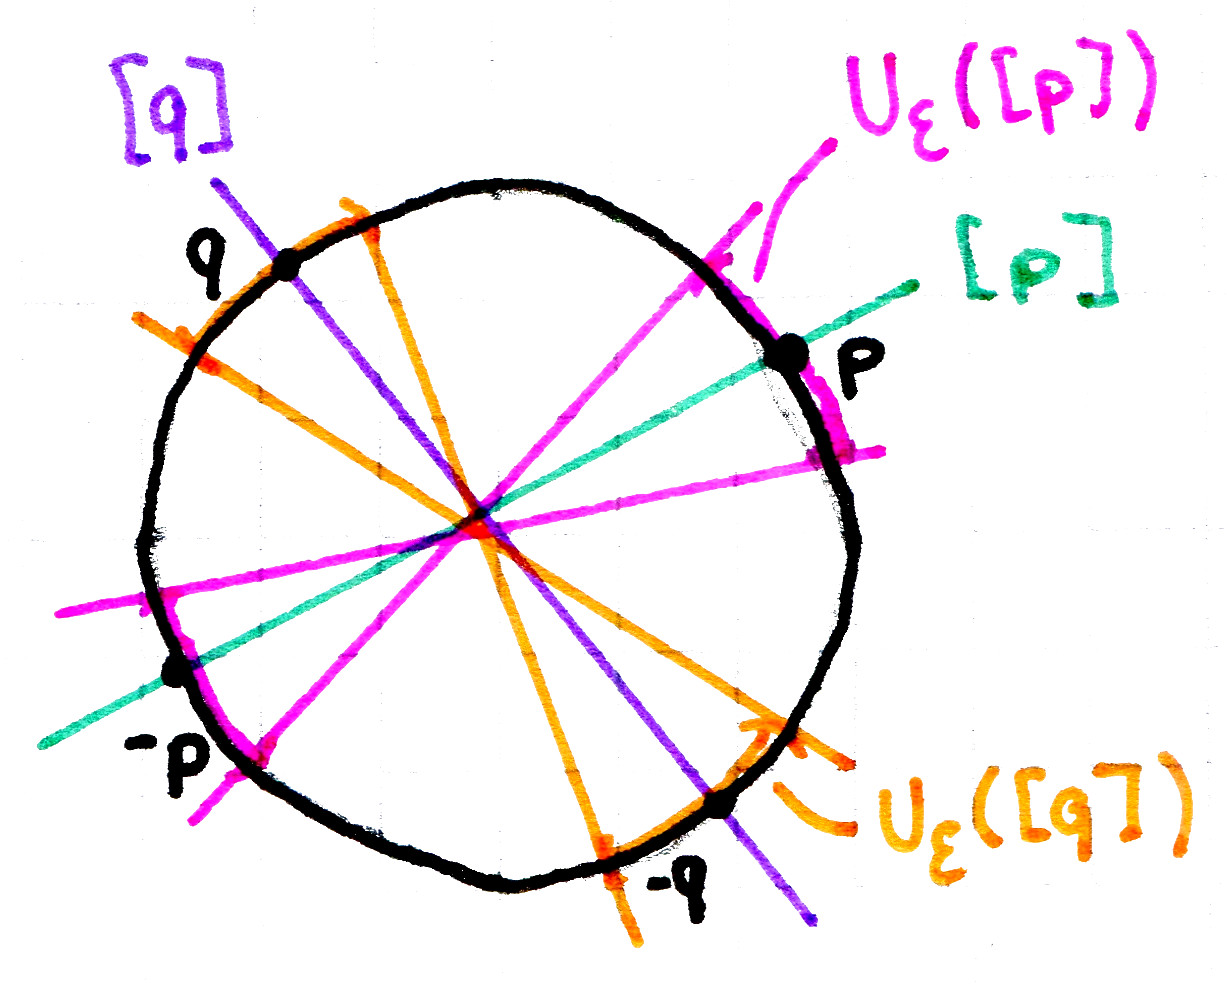
\includegraphics[width=.33\textwidth]{IdeeHausdorffsch}
    \caption{Idee zu Hausdorffsch}
  \end{figure}
\end{remark}

\begin{example}[Produkt-Mannigfaltigkeiten]
  Für \( M^m \) und \( N^n \) \( m \)- bzw. \( n \)-dimensionale differenzierbare Mannigfaltigkeit ist die \term{Produkt-Mannigfaltigkeit}\label{def:produktmannigfaltigkeit} \( M \times N \) eine \( (m+n) \)-dimensionale \( C^\infty \)-Mannigfaltigkeit.\footnote{\textbf{Übung}!}
\end{example}

\begin{excourse}[Lie-Gruppen]
  Eine \term{Lie-Gruppe}\label{def:liegruppe} ist eine Gruppe mit einer \( C^\infty \)-Mannigfaltigkeitstruktur, so dass die Abbildung
  \begin{equation*}
    G \times G \to G, \quad (g,h) \mapsto gh^{-1}
  \end{equation*}
  \( C^\infty \) ist.
\end{excourse}

\begin{example}[zu Lie-Gruppen]
  \
  \begin{itemize}
    \item \( (\Z, +) \) ist eine \( 0 \)-dimensionale Lie-Gruppe.
    \item \( SO(2) = \left \{ \begin{pmatrix}
      \cos \theta & -\sin \theta \\
      \sin \theta & \cos \theta
    \end{pmatrix} : \theta \in [0, 2\pi] \right \} \underset{\text{homö}}{\cong} S^1 \) ist kompakte \( 1 \)-dimensionale \( C^\infty \)-Mannigfaltigkeit und Lie-Gruppe.\footnote{\textbf{Übung}: Wieso?} 
    \item \( SU(2) \coloneqq \left \{ \begin{pmatrix}
      \alpha & \beta \\
      -\overline{\beta} & \overline{\alpha}
    \end{pmatrix} : \alpha, \beta \in \C, \ \alpha\overline{\alpha}+\beta\overline{\beta} = 1 \right \} \underset{\text{homö}}{\cong} S^3 \) ist kompakte \( 3 \)-dimensionale \( C^\infty \)-Mannigfaltigkeit.\footnote{\( 1 = \alpha\overline{\alpha}+\beta\overline{\beta} = x_1^2 + x_2^2 + x_3^2 + x_4^2 \) mit \( \alpha = x_1+\i x_2 \) und \( \beta = x_3 + \i x_4 \).}
    \item \( GL(n, \R) \) (offene) Untermannigfaltigkeit von \( \R^{n^2} \leadsto n^2 \)-dimensionale \( C^\infty \)-Mannigfaltigkeit.
  \end{itemize}
\end{example}

\begin{remark}[Fakt von Cartan]
  Abgeschlossene Untergruppen von Lie-Gruppen sind Lie-Gruppen sind auch Lie-Gruppen.
\end{remark}

\begin{example}[Fakt von Cartan benutzen]
  \
  \begin{align*}
    SO(n) &= \{ A \in GL(n, \R) : AA^\top = E, \ \det A = 1 \} \text{ und} \\
    SL(n, \R) &= \{ A \in GL(n, \R) : \det A = 1 \}
  \end{align*}
  sind Lie-Gruppen: Benutze, dass
  \begin{equation*}
    A = \{ x \in X : f(x) = g(x) \} \text{ und } X \text{ ist hausdorffsch}
  \end{equation*}
  \( \Rightarrow A \text{ abgeschlossen, } f, g \text{ stetige Abbildungen} \)
\end{example}

\section{Simplizialkomplexe}

Simplizialkomplexe sind Objekte der algebraischen Topologie. Mittels Kombinatorik sollen topologische Invarianten bestimmt werden.

\begin{definition}[Simplex]
  Ein \( k \)-dimensionales \term{Simplex}\label{def:simplex} im \( \R^n \) ist die konvexe Hülle von \( k+1 \) Punkten \( v_0, \dots, v_k \) in allgemeiner Lage:
  \begin{equation*}
    s(v_0, \dots, v_k) \coloneqq \left \{ \sum_{i=0}^n \lambda_i v_i : \forall \lambda_i \geq 0, \ \sum_{i = 0}^k \lambda_i = 1 \right \}
  \end{equation*}
  für \( v_0-v_1, \dots, v_0-v_k \) linear unabhängig.
\end{definition}

\begin{example}[Einfache Simplices]
  \
  \begin{itemize}
    \item \textbf{0-Simplex}: \( v_0 \) (Punkt) 
    \item \textbf{1-Simplex}: \( v_0 \) --- \( v_1 \) (Strecke, \( s(v_0, v_1) = \{ \lambda v_0 + (1-\lambda)v_1 : 0 \leq \lambda \leq 1 \} \))
    \item \textbf{2-Simplex}: \( \triangle v_0, v_1, v_2 \) (Dreiecksfläche)
    \item \textbf{3-Simplex}: \( v_0, v_1, v_2, v_3 \) ((volles) Tetraeder)
  \end{itemize}
  \begin{figure}[H]
    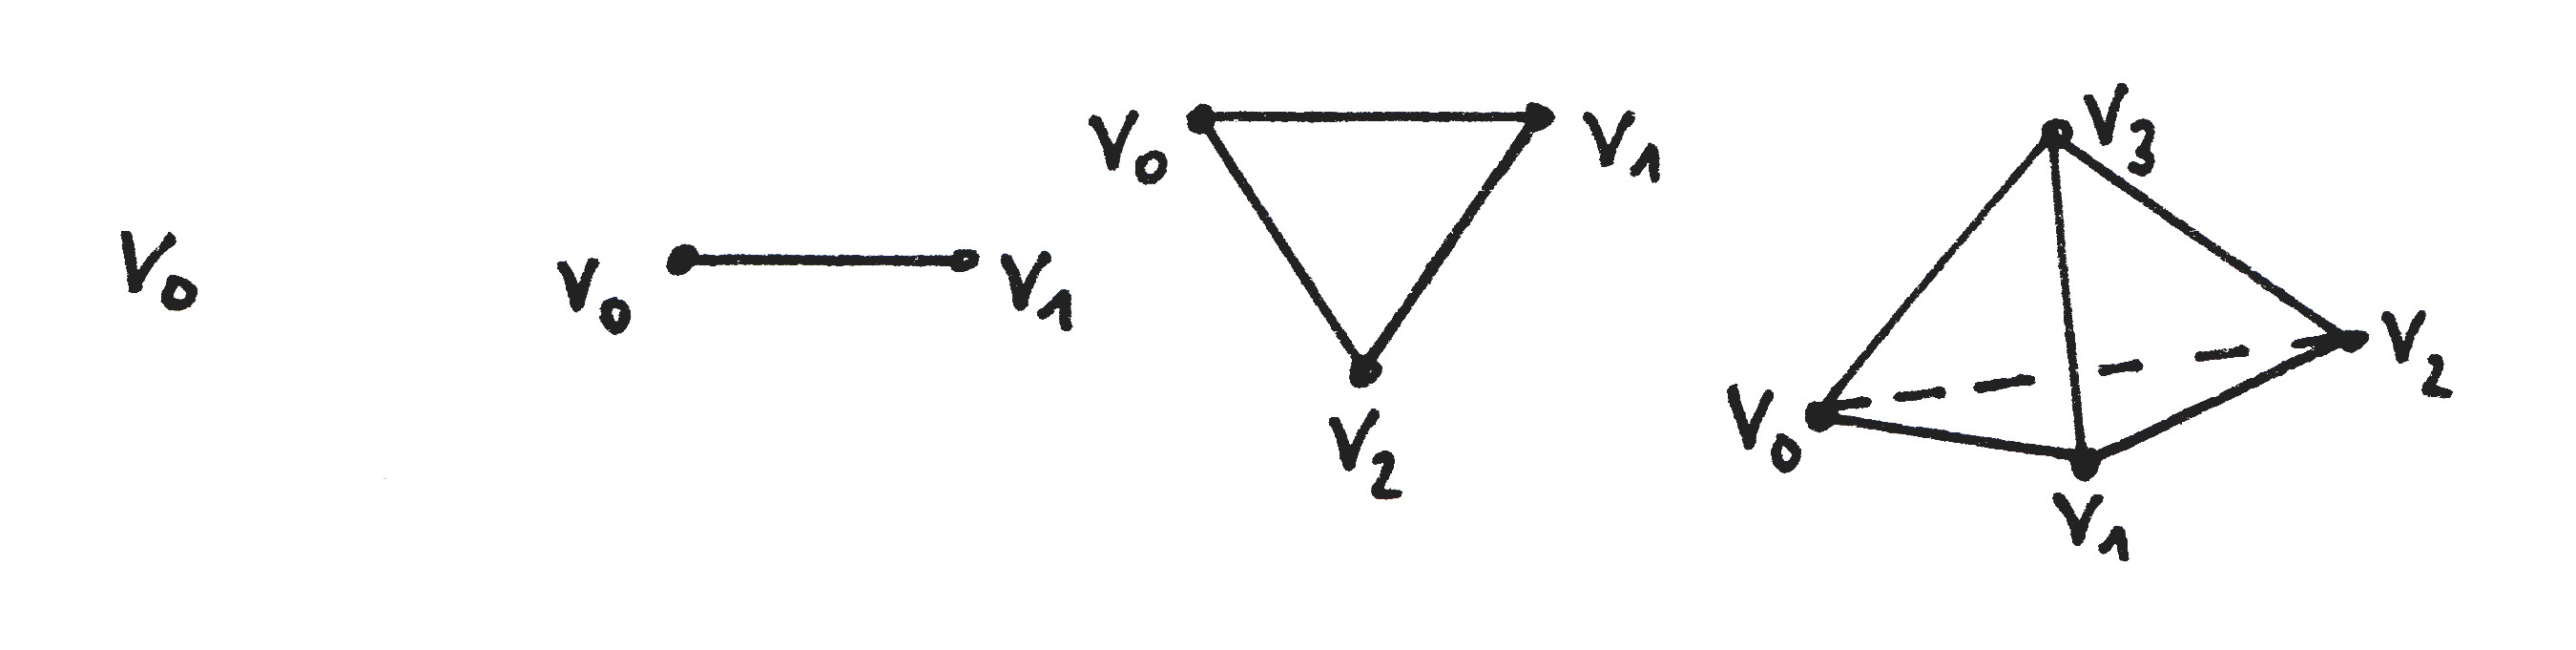
\includegraphics[width=.5\textwidth]{0123Simplex}
    \caption{\( 0 \)-, \( 1 \)-, \( 2 \)- und \( 3 \)-Simplex}
  \end{figure}
\end{example}

\begin{minipage}{.45\textwidth}
  \begin{definition}[Teilsimplex, Seite]
    Die konvexe Hülle einer Teilmenge von \( \{ v_0, \dots, v_k \} \) heißt \term{Teilsimplex}\label{def:seite} oder \term{Seite} von \( s(v_0, \dots, v_k) \).
  \end{definition}
\end{minipage}
\hfill
\begin{minipage}{.45\textwidth}
  \begin{figure}[H]
    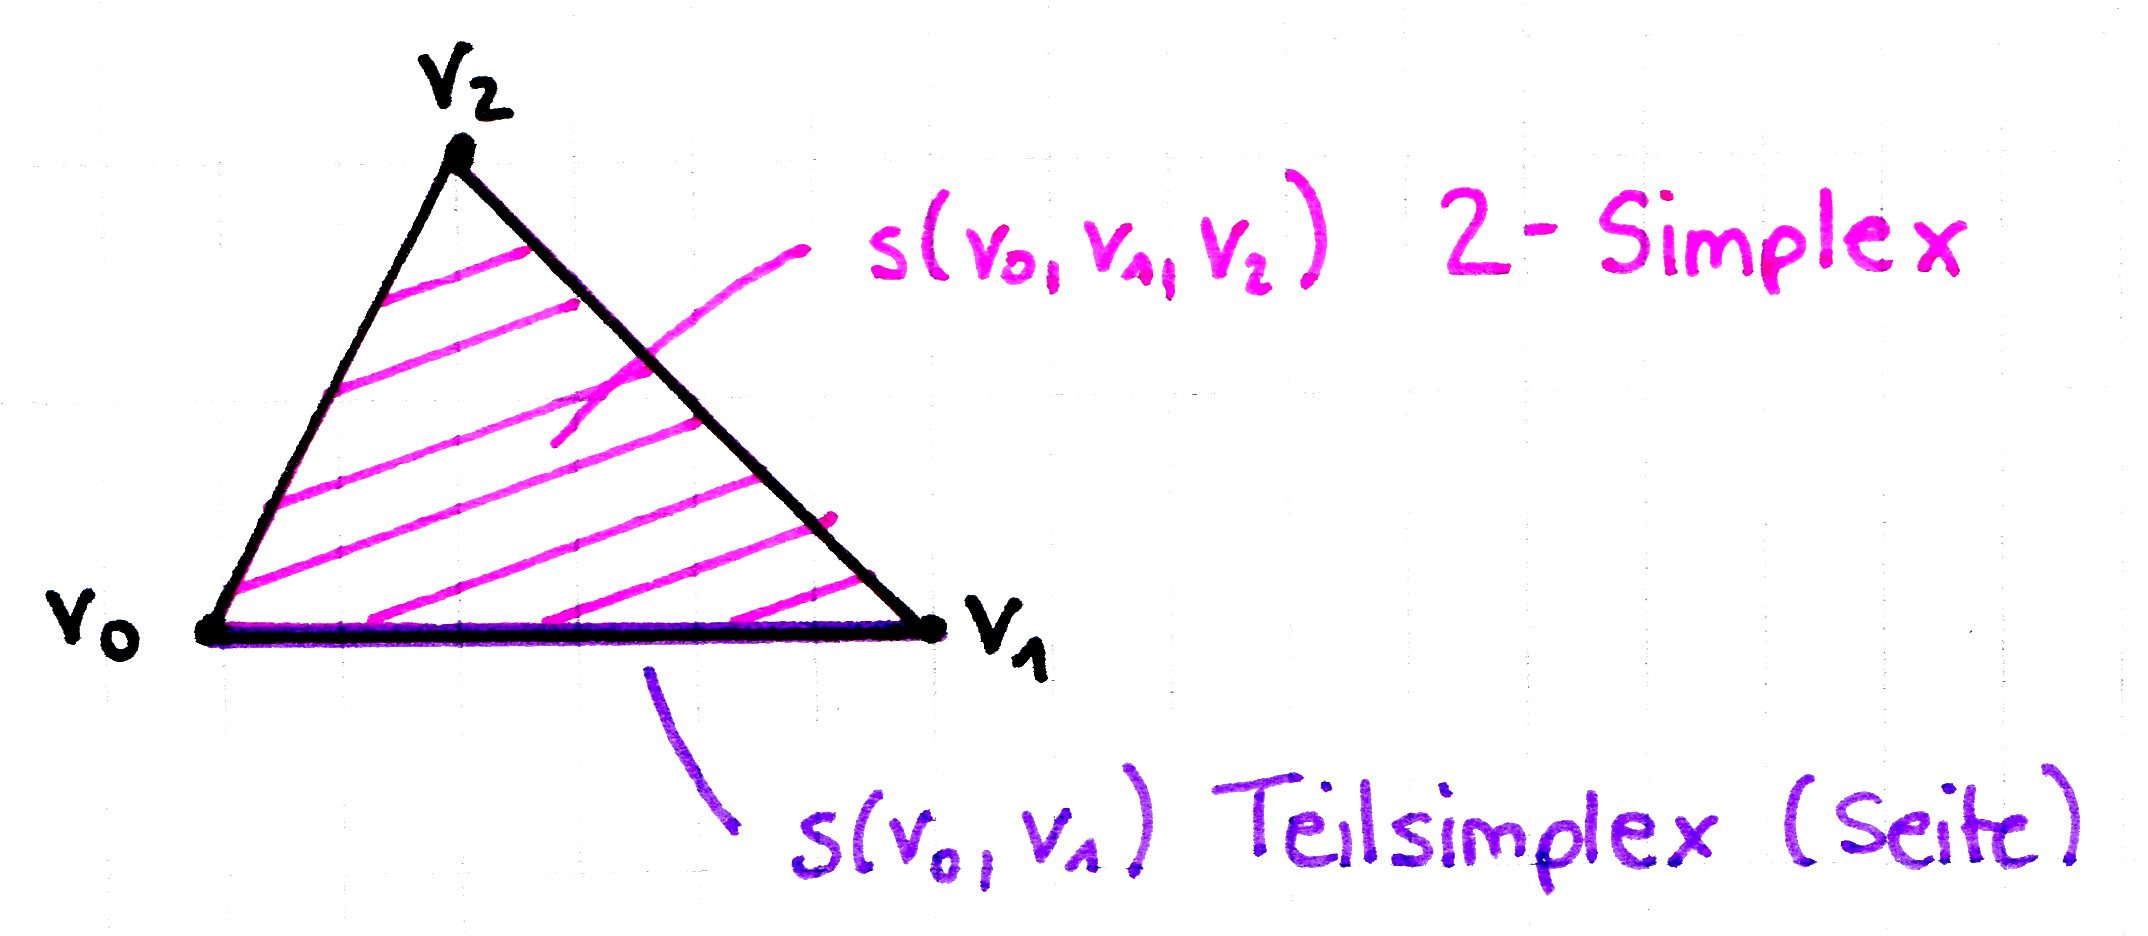
\includegraphics[width=\textwidth]{SimplexTeilsimplex}
    \caption{Simplex und Teilsimplex}
  \end{figure}
\end{minipage}

\begin{definition}[Simplizialkomplex]
  Eine endliche Menge \( K \) von Simplices in \( \R^n \) heißt \term{Simplizialkomplex}\label{def:simplizialkomplex}, wenn gilt:
  \begin{enumerate}
    \item Mit jedem seiner Simplices enthält \( K \) auch dessen sämtliche Teil-Simplices.
    \item Der Durchschnitt von je zwei Simplices ist entweder leer oder ein gemeinsamer Teilsimplex. 
  \end{enumerate}
  \begin{figure}[H]
    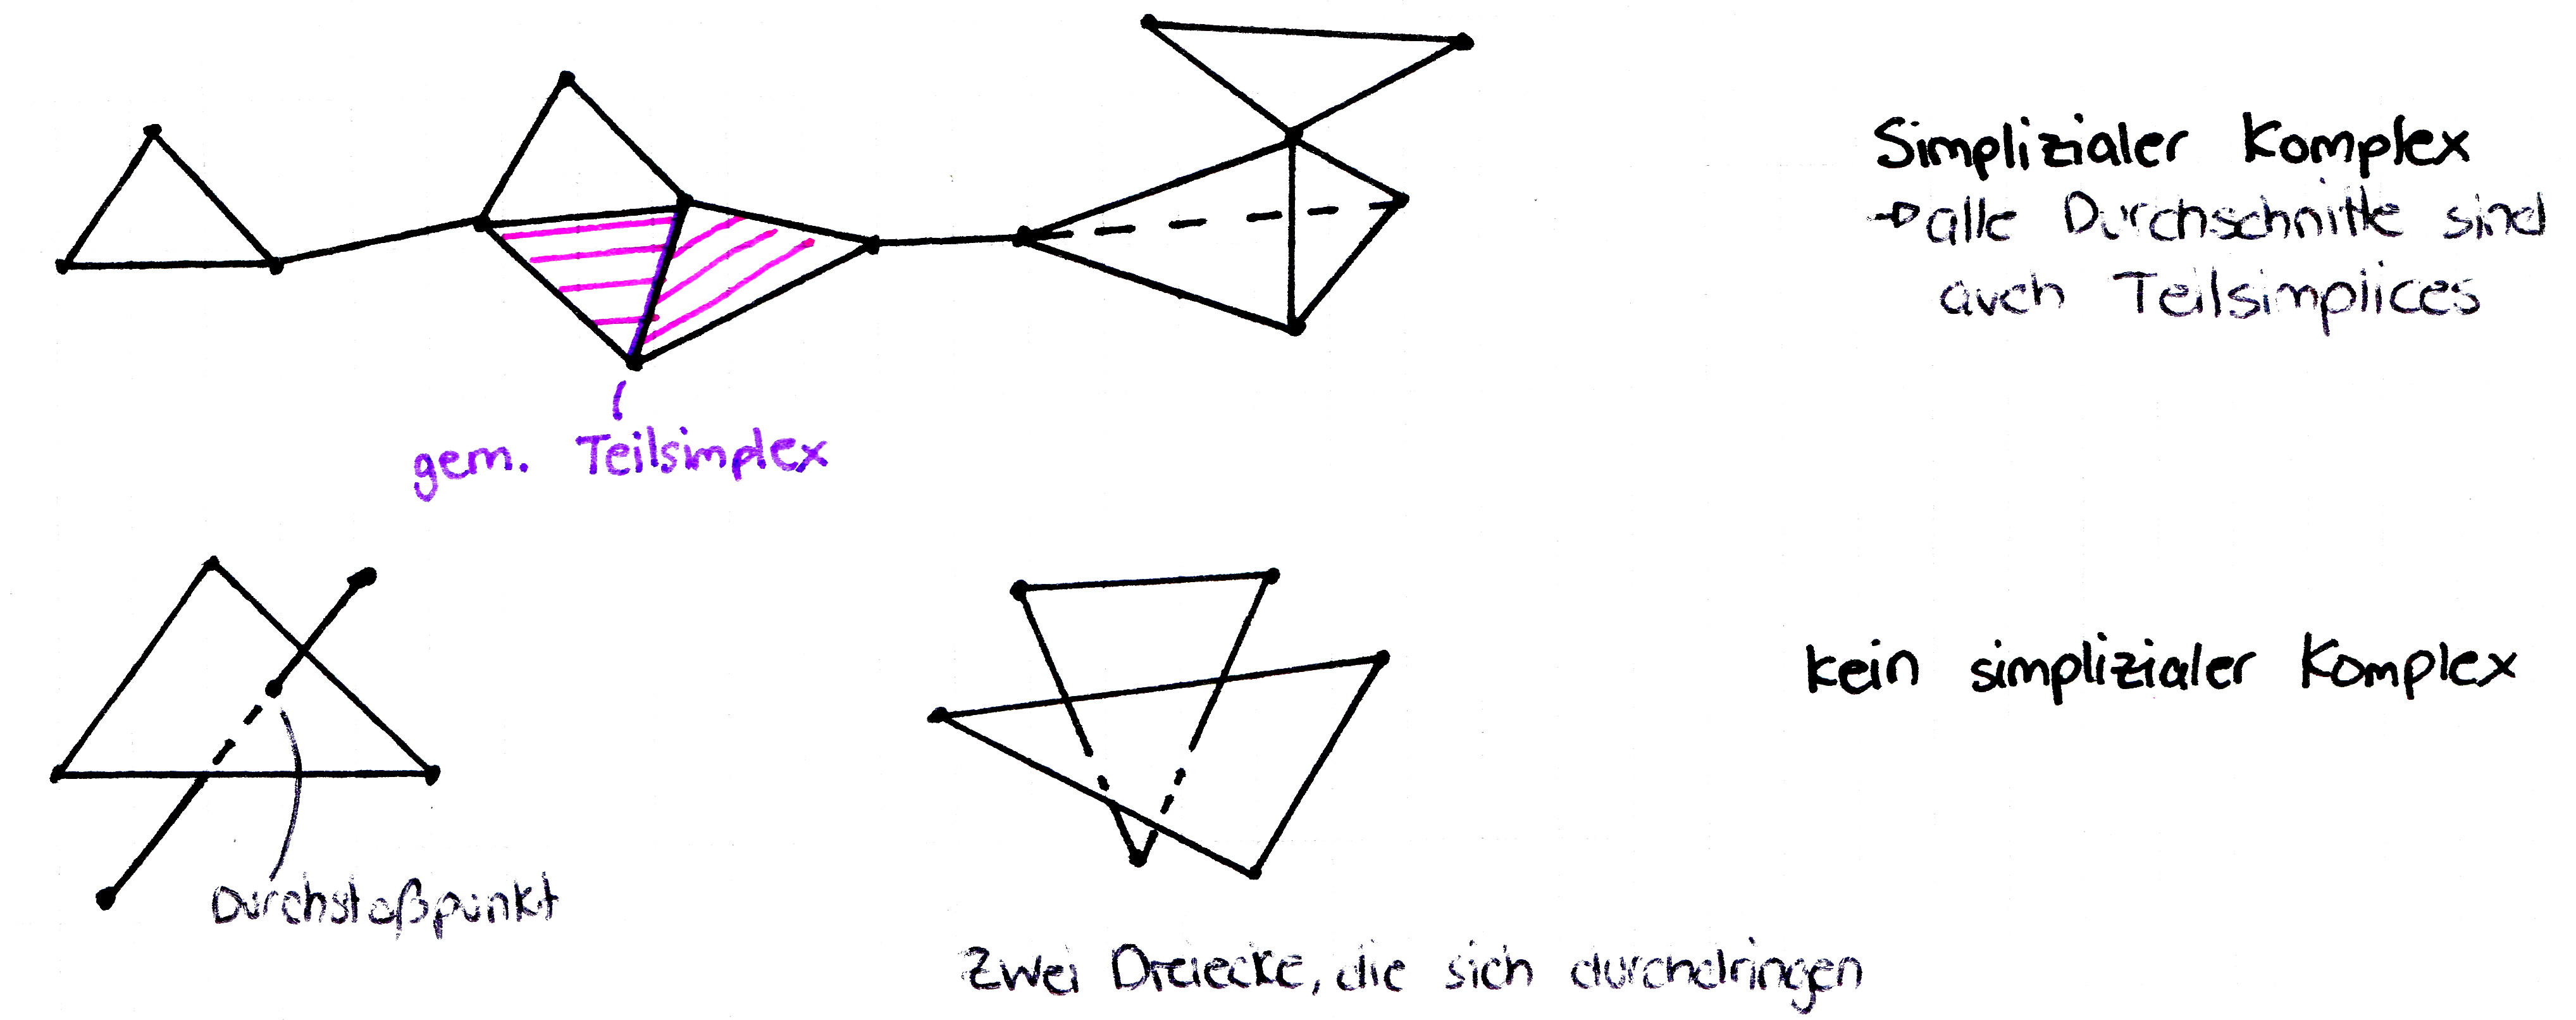
\includegraphics[width=.8\textwidth]{KeinSimplizialkomplex}
    \caption{Simplizialkomplex versus kein Simplizialkomplex}
  \end{figure}
\end{definition}

\begin{definition}[Geometrische Realisierung]
  \
  \begin{equation*}
    \vert K \vert \coloneqq \bigcup_{s \in K} s \subset \R^n
  \end{equation*}
  mit Teilraumtopologie von \( \R^n \) heißt der dem Simplizialkomplex \( K \) zugrunde liegende topologische Raum. \\
  \emph{Achtung}: Verschiedene Simplizialkomplexe \( K \), \( K' \) können das gleiche \( \vert K \vert = \vert K' \vert \) haben.
  % TODO Abbildung 1
\end{definition}

\begin{remark}[Vorteil von Simplizialkomplexen]
  Kennt man von einem (endlichen) Simplizialkomplex die \term{wesentlichen Simplices}\label{def:wesentlicheSimplices} (also solche, die nicht Seiten von anderen sind) in jeder Dimension und ihre \term{Inzidenzen}\label{def:inzidenzen} (also welche Ecken sie gemeinsam haben), so kennt man \( \vert K \vert \) (bis auf Homöomorphie).
  \begin{proof}[Konstruktionsidee von \( \vert K \vert \) aus diesen Daten]
    \
    \begin{enumerate}
      \item Wähle in jeder Dimension einen \emph{Standard-Simplex} \( \Delta_k \coloneqq s(\underbrace{e_1, \dots, e_{k+1}}_{\text{Std.-Basis-Vek.}}) \)
      \item Bilde disjunkte Vereinigung von solchen \( \Delta_k \) in jeder Dimension \( k \) so viele wie es wesentliche \( k \)-Simplices gibt:
        \begin{equation*}
          X \coloneqq \underbrace{\Delta_0 \cup \dots \cup \Delta_0}_{\text{\# wesentliche \( 0 \)-Simp.}} \cup \dots \cup \underbrace{\Delta_n \cup \dots \cup \Delta_n}_{\text{\# wesentliche \( n \)-Simp.}}
        \end{equation*}
      \item Identifiziere Inzidenzen (via Äquivalenzrelation) gemäß Inzidenz-Angaben für Ecken
    \end{enumerate}
    Diese drei Schritte liefern dann eine stetige Bijektion des (kompakten) Quotientenraumes \( X/\sim \) auf Hausdorff-Raum \( \vert K \vert \), also ein Homöomorphismus. \qed{}
  \end{proof}
\end{remark}

\begin{definition}[Dimension]
  Die \term{Dimension} eines Simplizialkomplexes \( K \) ist die maximale Dimension seiner Simplices.
\end{definition}

\begin{remark}[Spezialfall --- Graph]
  Ein \term{endlicher Graph}\label{def:graph} ist ein endlicher, \( 0 \)- oder \( 1 \)-dimensionaler Simplizialkomplex,\footnote{Aufgrund der Eindimensionalität haben beispielsweise die Dreiecke in einem Graph keine Füllung!} gebaut aus \( 1 \)-dimensionalen (\emph{Kanten}) und \( 0 \)-dimensionalen (\emph{Ecken}) Simplices. \\
  Ein Graph \( G \) heißt \term{zusammenhängend}\label{def:zusammenhaengend}, falls zu je zwei Ecken \( p, p' \in G \) eine Folge \( p = p_0, p_1, \dots, p_n = p' \) paarweise verschiedener Ecken von \( G \) existiert, sodass \( p_{i-1} \) und \( p_i \) durch eine Kante verbunden sind. \\
  Ein \term{Baum}\label{def:baum} ist ein zusammenhängender Graph \( T \), so dass für jedes \( 1 \)-Simplex (\emph{Kante}) \( s \in T \) gilt: \( \vert T \vert \setminus \mathring{s} \) ist nicht zusammenhängend (mit \( \mathring{s} = \) \emph{offener} \( 1 \)-Simplex, also Kante ohne Endpunkte).
\end{remark}

\begin{definition}[Euler-Charakteristik]
  Sei \( G \) ein endlicher Graph,
  \begin{align*}
    \alpha_0 &\coloneqq \text{ Anzahl Ecken in } G\text{,} \\
    \alpha_1 &\coloneqq \text{ Anzahl Kanten in } \text{G.}
  \end{align*}
  Die \term{Euler-Charakteristik}\label{def:eulerCharakteristik} von \( G \) ist
  \begin{equation*}
    \chi(G) \coloneqq \alpha_0 - \alpha_1
  \end{equation*}
  \emph{Bemerkung}: \( \chi(G) \) ist invariant unter Unterteilung (also dem Hinzufügen von neuen Ecken auf einer Kante).
\end{definition}

\begin{theorem}[\( \chi \) von Bäumen]
  Sei \( T \) ein (endlicher) Baum. Dann gilt \( \chi(T) = 1 \).
  \begin{proof}
    Induktion nach \( \alpha_0 = \) Anzahl Ecken.
    \begin{itemize}
      \item \( n = 1 \). Dann ist \( G \) ein Punkt, \( \alpha_0 = 1 \), \( \alpha_1 = 0 \), \( \chi(T) = \alpha_0 - \alpha_1 = 1 \quad \checkmark \)
      \item \( n = 2 \). Dann ist \( G \) eine Kante mit Endpunkten, \( \alpha_0 = 2 \), \( \alpha_1 = 1 \), \( \chi(T) = 1 \quad \checkmark \)
      \item \textbf{Induktionsannahme}: Satz gilt für alle Bäume mit \( n \) Ecken.
      \item \textbf{Induktionsschritt}: \( \chi(T) = 1 \) für Bäume mit \( n+1 \) Ecken. \\
        Sei \( T \) ein Baum mit \( n+1 \) Ecken und \( v_0 \) ein \term{Ende}\label{def:blatt} von \( T \) (also eine Ecke die zu genau einer Kante gehört). Ein solches Ende existiert.\footnote{vgl. Übung} \\
        Sei \( \vert T_1 \vert \coloneqq \vert T \vert \setminus \{ \mathring{s_1} \cup v_0 \} \). \( T_1 \) ist wieder ein Baum, sonst existiert \( s_2 \) sodass \( T_1 \setminus \{ \mathring{s_2} \} \) zusammenhängend ist, also auch \( T \setminus \{ \mathring{s_2} \} \) zusammenhängend \( \lightning \). \\
        \( T_1 \) hat \( n \) Ecken, also nach IV:\@ \( \chi(T_1) = 1 \). \\
        Da \( \alpha_0(T) = \alpha_0(T_1) + 1 \) und \( \alpha_1(T) = \alpha_1(T_1) + 1 \) ist \( \chi(T_1) = 1 \). \qed{}
    \end{itemize}
  \end{proof}
\end{theorem}

\begin{theorem}[\( \chi \) von zusammenhängenden Graphen]
  Sei \( G \) ein zusammenhängender, endlicher Graph. Sei \( n \) die Anzahl von offenen \( 1 \)-Simplices (\emph{Kanten}), die man aus \( G \) entfernen kann, sodass \( G \) zusammenhängend bleibt. Dann ist \( \chi(G) = 1 - n \).\footnote{Die Aussage aus dem vorhergehenden Satz folgt aus diesem direkt.}
  \begin{proof}
    Ist \( G \) ein Baum, so ist \( n = 0 \) und die Behauptung gilt. \\
    Ist \( G \) \underline{kein} Baum, so existiert ein offenes \( 1 \)-Simplex \( \mathring{s_1} \), sodass \( \vert G_1 \vert = \vert G \vert \setminus \{ \mathring{s_1} \} \) zusammenhängend ist. Ist \( G_1 \) ein Baum, so hält man an. Ist \( G_1 \) kein Baum, so entfernt man eine Kante \( \mathring{s_2} \) und so weiter. \\
    \( G \) hat endlich viele Kanten, also existiert ein maximales \( n \), so dass \( \vert G \vert \setminus \{ \mathring{s_1} \cup \cdots \cup \mathring{s_n} \} \) ein Baum ist. \\
    Es gilt dann \( \chi(G) = \chi(T) - n = 1-n \). \qed{}
  \end{proof}
  \emph{Bemerkung}: Das Komplement \( T \) aller offenen Kanten die man aus \( G \) entfernen kann (wie im Beweis) ist ein sog. \term{spannender Baum}\label{def:spannenderBaum} für \( G \), der alle Ecken in \( G \) enthält (nicht eindeutig).
\end{theorem}

\begin{definition}[Ebene und planare Graphen]
  Ein Graph heißt \term{eben}\label{def:eben}, falls er durch Punkte und Geradenstücke in der Ebene (also \( \R^2 \)) realisiert ist, so dass sich die Kanten nicht schneiden (außer in den Ecken). \\
  Ein (abstrakter) Graph (also gegeben durch Ecken-Mengen und Inzidenzen) heißt \term{planar}\label{def:planar}, falls er \emph{isomorph} zu einem ebenen Graphen ist.  
\end{definition}

\begin{example}
  \
  \begin{enumerate}
    \item \( K_4 = \) vollständiger Graph mit \( 4 \) Ecken (also sind alle Ecken-Paare durch Kanten verbunden). Zeichnet man diesen Graphen als Quadrat, so ist dieser nicht eben. Man kann aber \( K_4 \) so zeichnen, dass der Graph eben ist. Also ist \( K_4 \) planar.
    \item \( K_5 = \) vollständiger Graph mit \( 5 \) Ecken. Dieser Graph ist nicht isomorph zu einem ebenen Graphen, also ist \( K_5 \) nicht planar.
  \end{enumerate}
  \begin{figure}[H]
    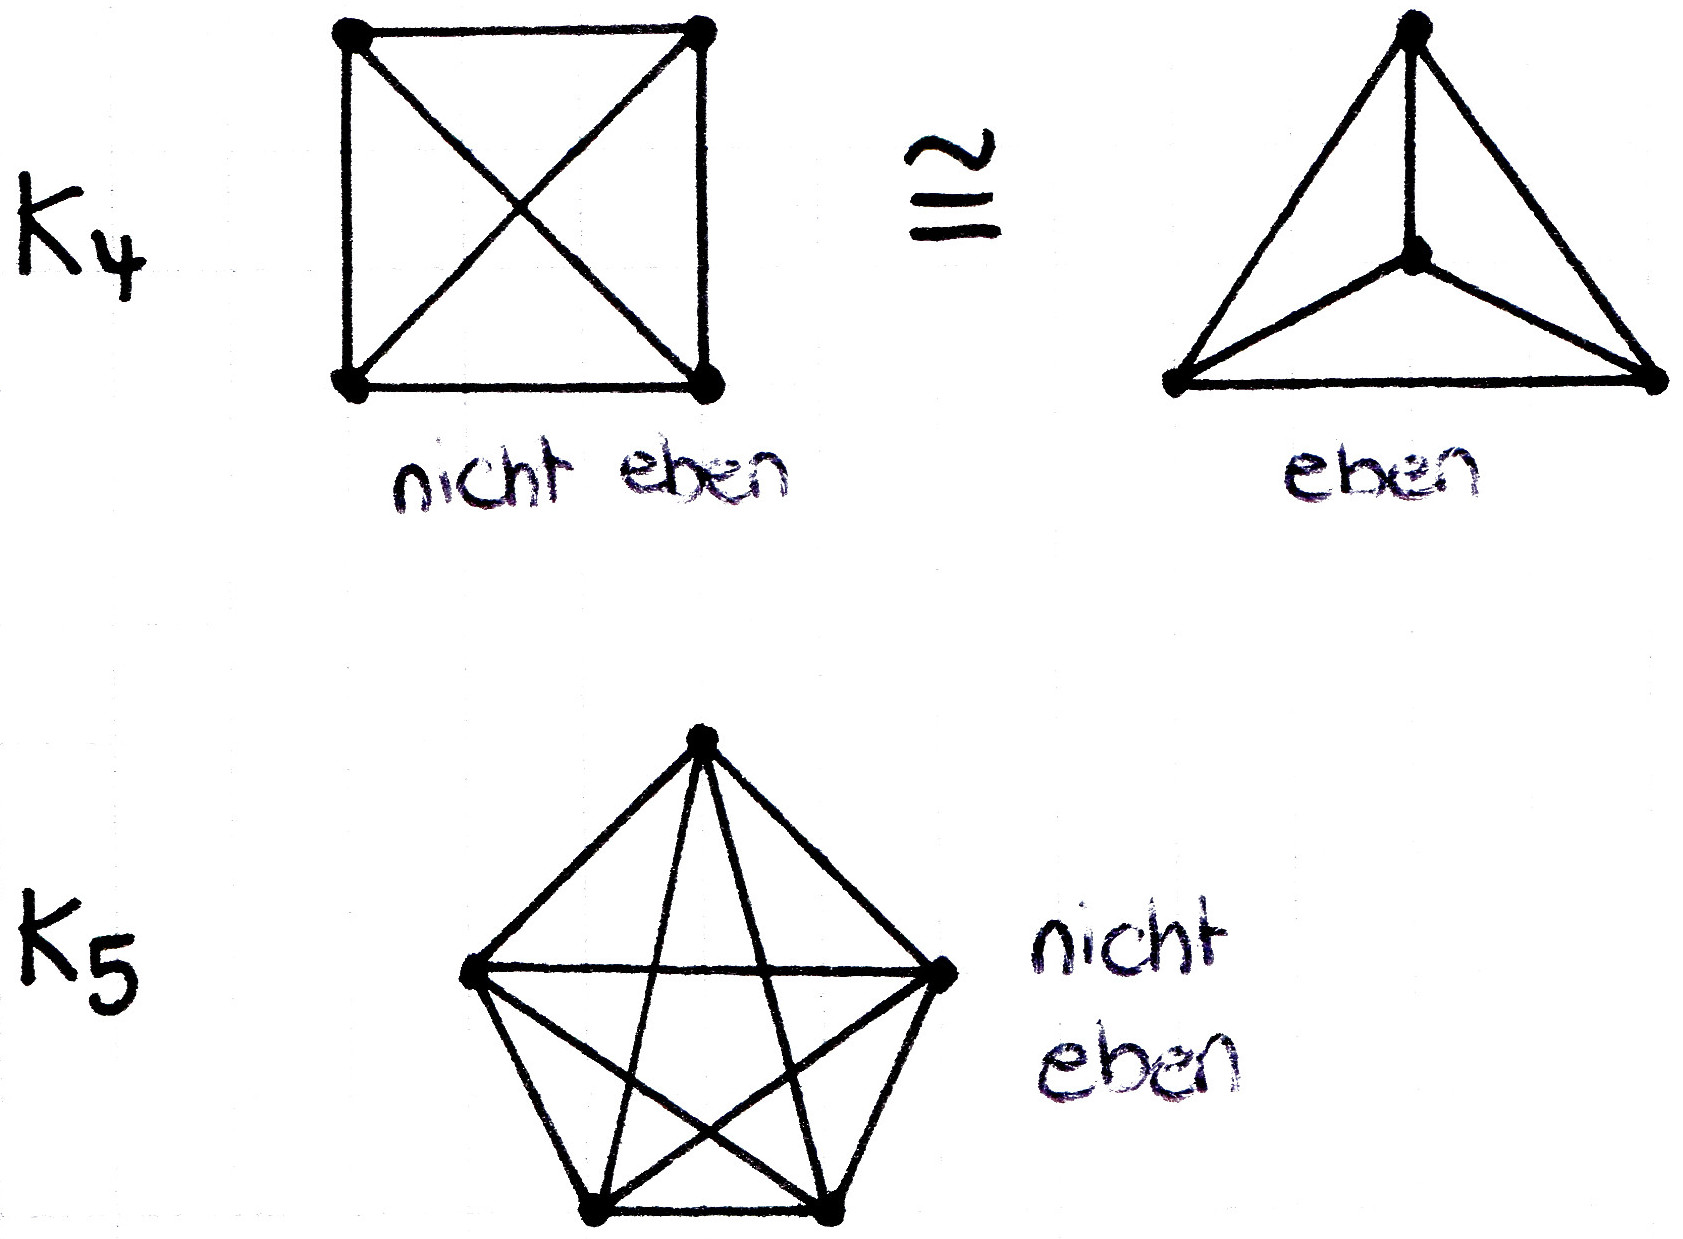
\includegraphics[width=.33\textwidth]{NichtPlanar}
    \caption{Planar versus nicht planar}
  \end{figure}
\end{example}

\begin{minipage}{.45\textwidth}
  \begin{definition}[Seiten]
    Die \term{Seiten}\label{def:seiten} eines ebenen Graphen \( G \) sind die Zusammenhangskomponenten von \( \R^2 \setminus G \).
  \end{definition}
\end{minipage}
\hfill
\begin{minipage}{.45\textwidth}
  \begin{figure}[H]
    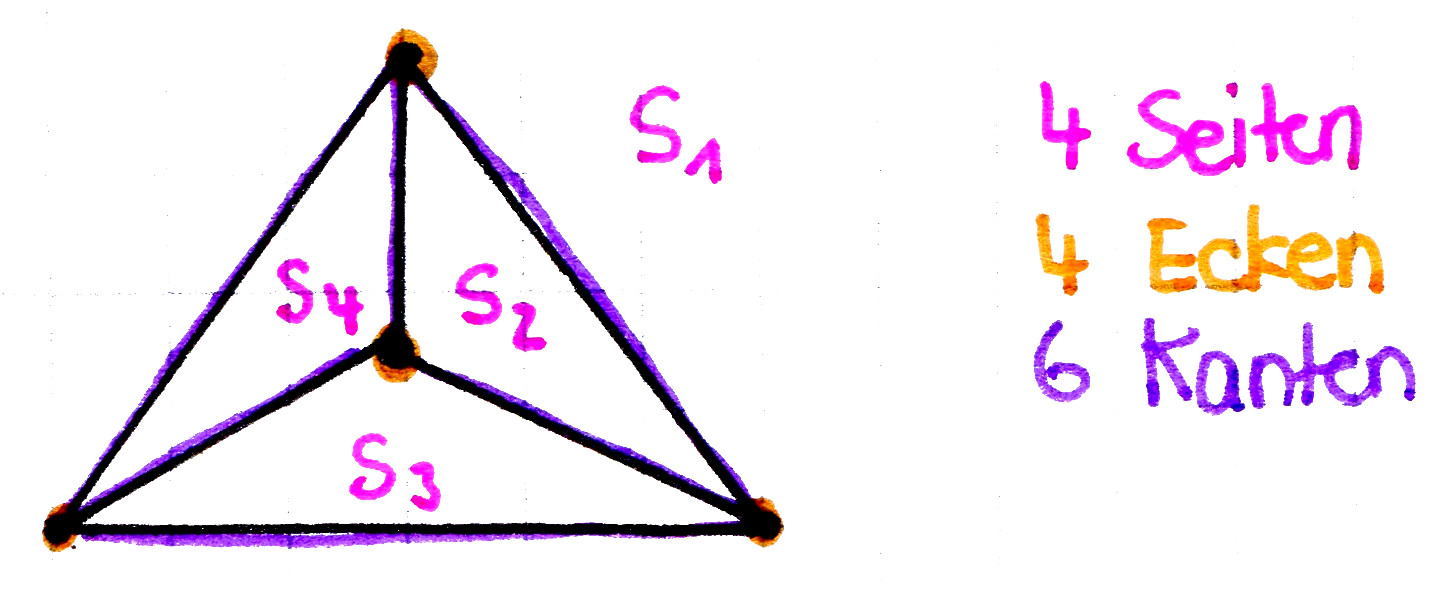
\includegraphics[width=.8\textwidth]{SeitenEckenKanten}
    \caption{Seiten, Ecken und Kanten eines Graphen}
  \end{figure}
\end{minipage}

\begin{theorem}[Euler-Formel]
  Für einen zusammenhängenden, ebenen Graphen \( G \) gilt:
  \begin{equation*}
    \chi(G) \coloneqq e(G) - k(G) + s(G) = 2\text{,}
  \end{equation*}
  wobei \( e(G) \) die Anzahl Ecken von \( G \), \( k(G) \) die Anzahl Kanten von \( G \) und \( s(G) \) die Anzahl Seiten von \( G \) ist. \\
  \( \chi(G) \) ist die \term{Euler-Charakteristik}\label{def:eulercharakteristik} von \( G \).
  \begin{proof}
    Sei \( T \) ein \term{aufspannender Baum}\label{def:aufspannenderBaum} für \( G \) (also ein Baum der alle Ecken von \( G \) enthält). Dann gilt \( e(T)-k(T) = 1 \) und \( s(T) = 1 \). Also gilt die Behauptung für \( T \). \\
    \( G \) erhält man aus \( T \) durch Hinzufügen von Kanten. Für jede neue Kante entsteht auch eine neue Seite, welche sich in der Summe aus der Behauptung aufheben. Also
    \begin{equation*}
      \chi(G) = e(G)-k(G)+s(G) = 2\text{.}
    \end{equation*}\qed{}
  \end{proof}
\end{theorem}

\begin{definition}[Polyeder]
  Eine Teilmenge \( P \) von \( \R^3 \) heißt \term{(konvexes) Polyeder}\label{def:polyeder}, falls
  \begin{enumerate}
    \item \( P \) ist Durchschnitt von endlich vielen \term{affinen Halbräumen}\label{def:affinerHalbraum} von \( \R^3 \) (also gegeben durch Ungleichungen \( {a_i}x+{b_i}y+{c_i}z \geq d_i \), \( i = 1, \dots, k \))
    \item \( P \) ist beschränkt und nicht in einer Ebene enthalten.
  \end{enumerate}

  \begin{minipage}{.45\textwidth}
    Der \term{Rand}\label{def:rand} von \( P \) besteht dann aus Seiten(-flächen), Kanten und Ecken (gegeben als \( 2 \)-dimensionale, \( 1 \)-dimensionale und \( 0 \)-dimensionale Schnitte von Ebenen).
  \end{minipage}
  \hfill
  \begin{minipage}{.45\textwidth}
    \begin{figure}[H]
      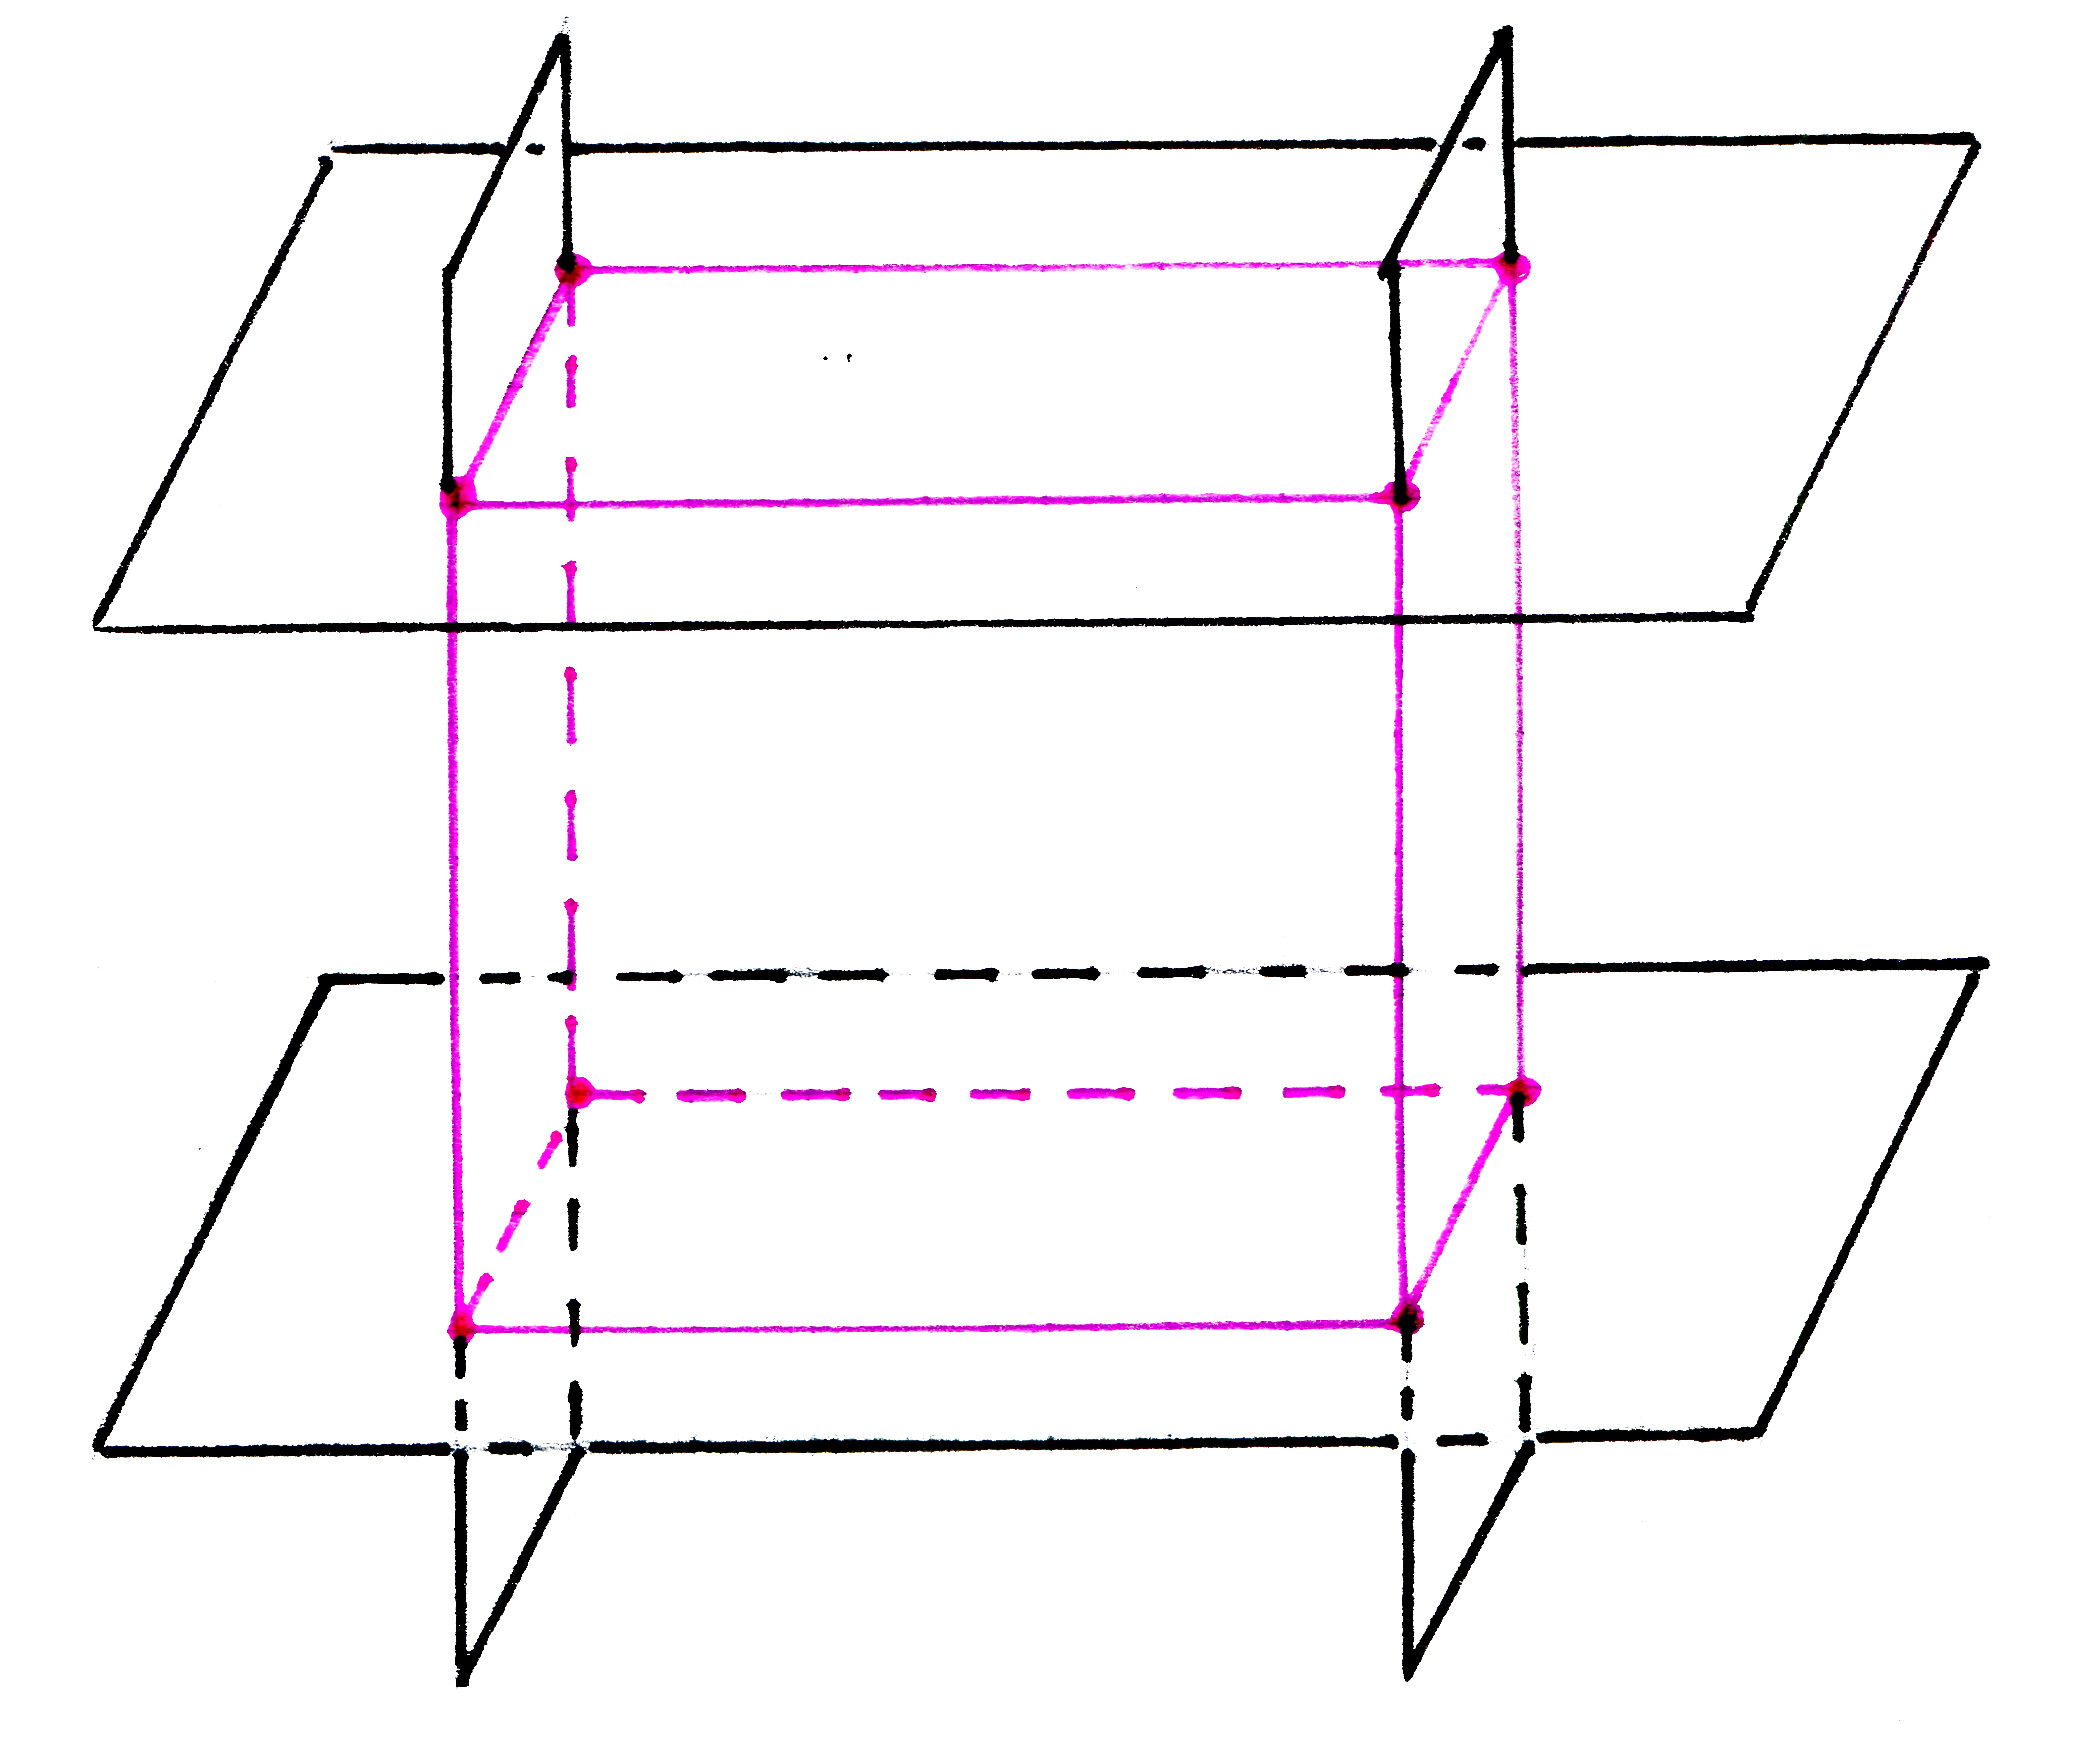
\includegraphics[width=.8\textwidth]{VollerWuerfel}
      \caption{Ein voller Würfel, beschränkt durch seine Seitenflächen. Vorder- und Rückseite sind zur Übersichtlichkeit weggelassen}
    \end{figure}
  \end{minipage}
\end{definition}

\begin{remark}[Bezug von Polyedern zu Graphen]
  Das \term{1-Skelett}\label{def:skelett} von \( P \) (also die Menge der Ecken und Kanten) von \( P \) ist ein Graph in \( \R^3 \). \\
  Man kann zeigen (Resultat der konvexen Geometrie): durch Zentralprojektion von einem Punkt nahe bei einem ``Seitenmittelpunkt'' auf eine geeignete Ebene wird das \( 1 \)-Skelett \( p^{(1)} \) von \( P \) auf einen \emph{ebenen} Graphen \( G_p \) abgebildet (sog. \term{Schlegel-Diagramm}\label{def:schlegelDiagramm}). Es gilt dann: \( s(P) = s(G_p) \), \( k(P) = k(G_p) \), \( e(P) = e(G_p) \).
  \begin{figure}[H]
    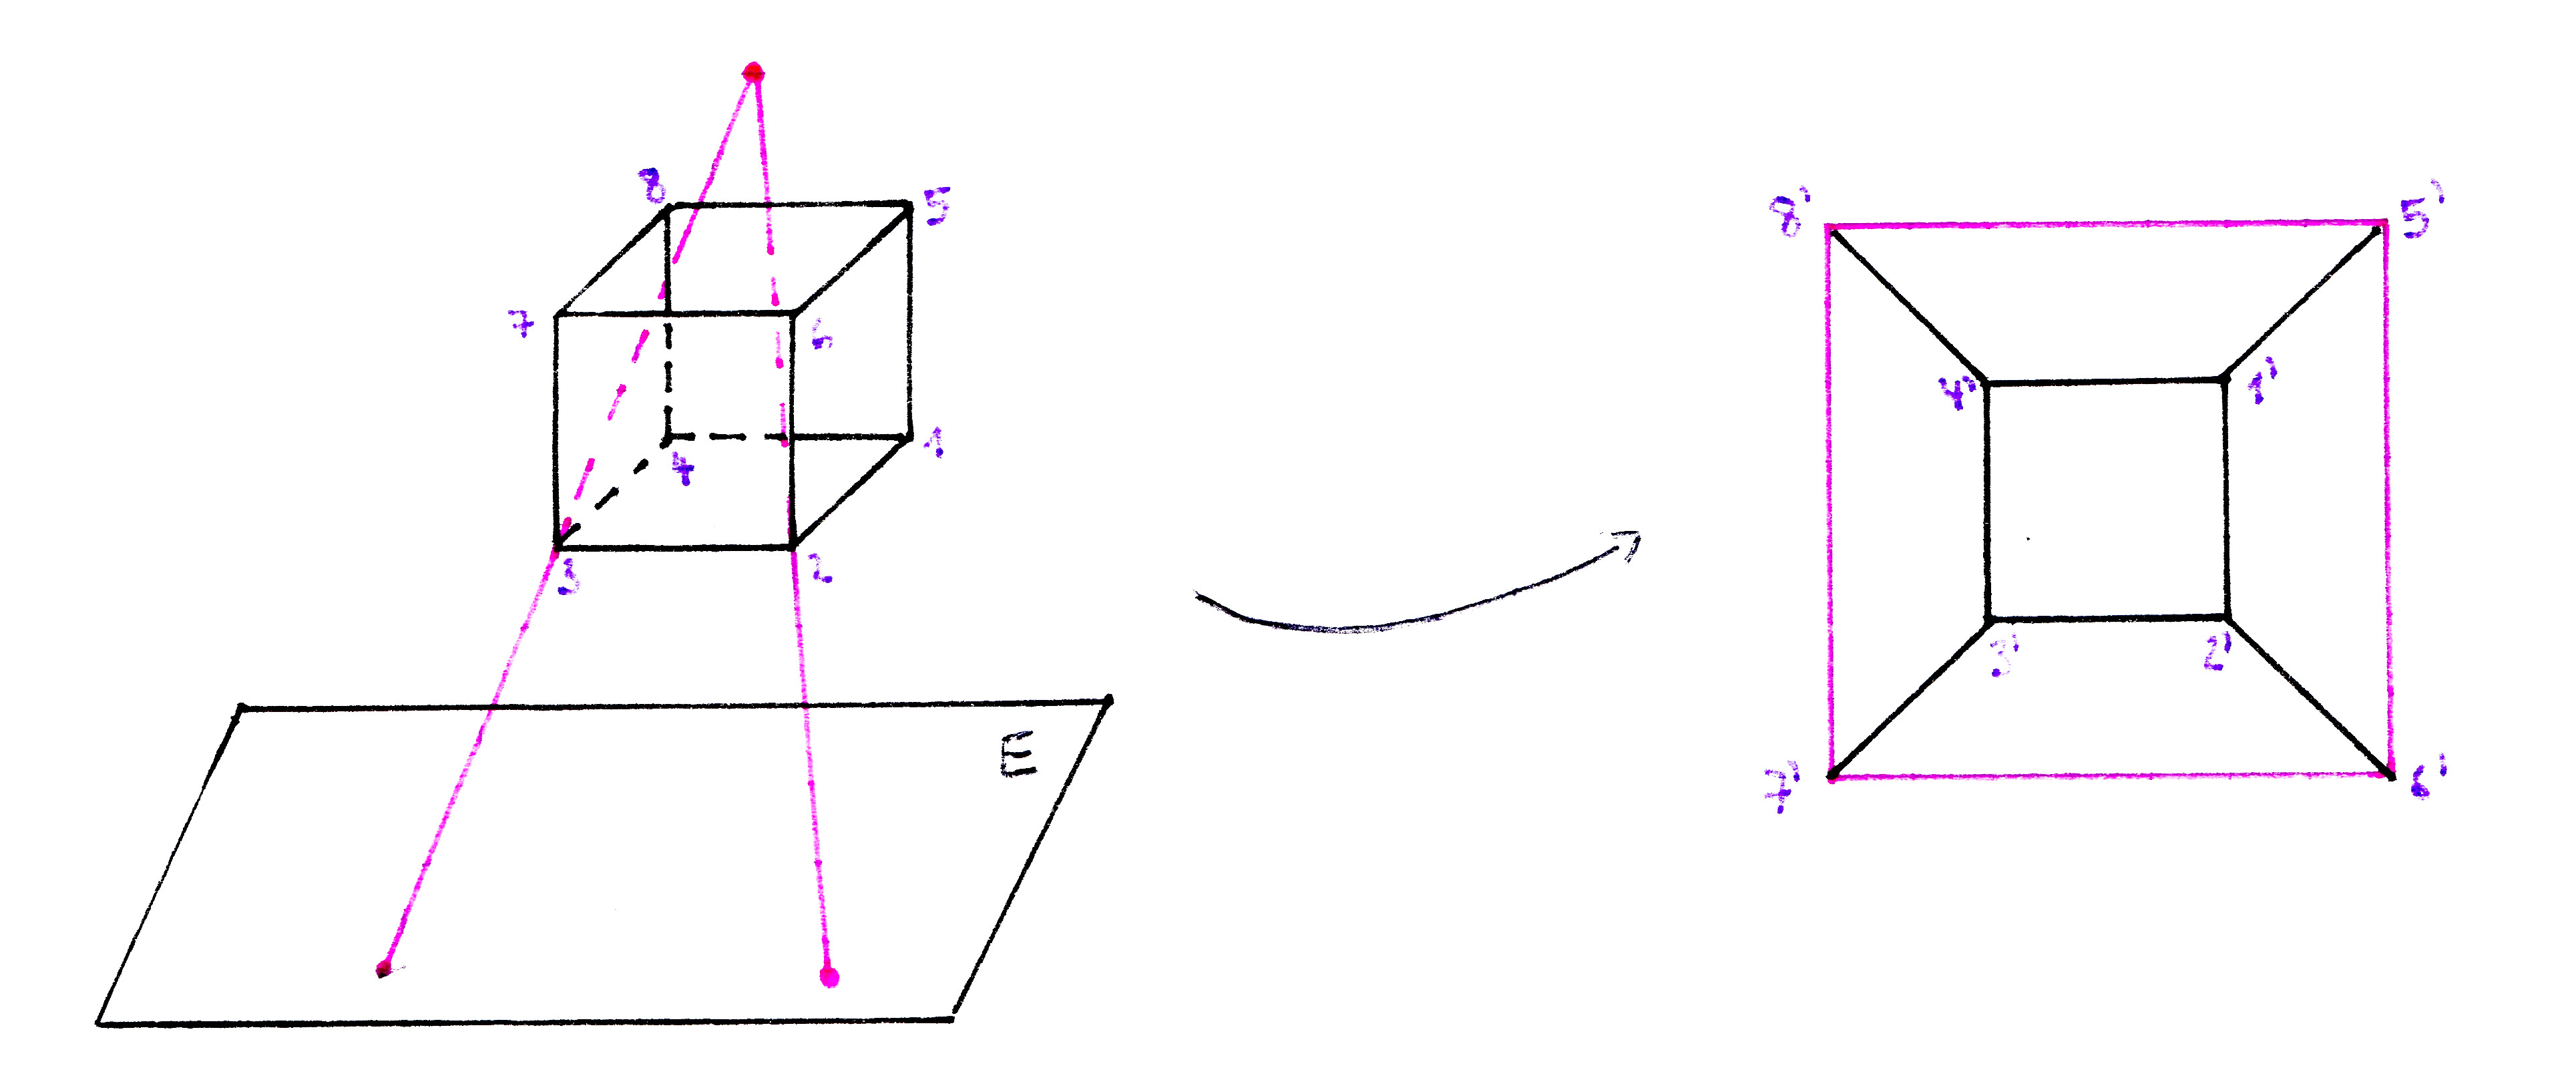
\includegraphics[width=.8\textwidth]{VollerWuerfelEbene}
    \caption{Projektion des vollen Würfels auf die Ebene}
  \end{figure}
\end{remark}

\begin{deduction}[Eulersche Polyeder-Formel]
  \begin{equation*}
    e(P) - k(P) + s(P) = 2\text{.}
  \end{equation*}
\end{deduction}

\begin{definition}[Regulärer Polyeder]
  Ein Polyeder in \( \R^3 \) heißt \term{regulär}\label{def:regulaererPolyeder}, falls alle Seitenflächen kongruente reguläre \( n \)-Ecke (also haben sie gleich lange Kanten) sind und in jeder Ecke \( m \) solche \( n \)-Ecke zusammentreffen (insbesondere gehen von jeder Ecke \( m \) Kanten aus).
\end{definition}

\begin{theorem}[Platonische Körper]
  Es gibt genau \( 5 \) reguläre Polyeder in \( \R^3 \):
  \begin{align*}
    (m,n) &= (3,3) \quad \text{Tetraeder}  \\
     &= (3,4) \quad \text{Würfel} \\
     &= (4,3) \quad \text{Oktaeder} \\
     &= (3,5) \quad \text{Dodekaeder} \\
     &= (5,3) \quad \text{Ikosaeder}
  \end{align*}
  \begin{proof}
    \
    \begin{itemize}
      \item \textbf{Existenz}: Explizite Konstruktion, siehe Euklid (oder Tutorium (oder basteln (oder Google))).
      \item \textbf{Vollständigkeit}: Sei \( s = \) Anzahl an Seitenflächen. Dann gilt: \( s*n = 2k \), ebenso \( m*e = 2k \) und damit
        \begin{equation*}
          n*s = 2k = m*e \Rightarrow k = \frac{me}{2} \quad s = \frac{me}{n}
        \end{equation*}
        Euler-Polyeder-Formel für \( P \) beziehungsweise \( G_p \) ergibt:
        \begin{equation*}
          2 = e-k+s = e - \frac{me}{2} + \frac{me}{n} \Leftrightarrow 4n = e\left( 2n - nm + 2m \right)\text{.}
        \end{equation*}
        Da \( n > 0 \) und \( e > 0 \) folgt:
        \begin{equation*}
          2n - nm + 2m > 0 \Leftrightarrow nm - 2n - 2m + 4 < 4 \Leftrightarrow (n-2)(m-2) < 4\text{.}
        \end{equation*}
        Man sieht, dass es nur obenstehende Möglichkeiten gibt. \qed{}
    \end{itemize}
  \end{proof}
\end{theorem}

\begin{definition}[Euler-Charakteristik von Simplizialkomplexen]
  Sei \( K \) ein Simplizialkomplex. Dann ist die \term{Euler-Charakteristik}\label{def:eulercharakteristikSimplizialkomplex} von \( K \):
  \begin{equation*}
    \chi(K) \coloneqq \alpha_0-\alpha_1+\alpha_2 \mp \dots \pm \alpha_k = \sum_{i = 0}^k {(-1)}^i\alpha_i\text{,}
  \end{equation*}
  wobei \( \alpha_i = \) Anzahl von \( i \)-Simplices in \( K \). \\
  Die sogenannten ``\term{Betti-Zahlen}''\label{def:bettiZahlen} lassen sich berechnen mit Methoden aus der algebraischen Topologie (als Dimension von gewissen Vektorräumen, die man zu \( K \) konstruiert). \\
  Man zeigt: \( \chi(K) \) ist eine topologische Invariante, also 
  \begin{equation*}
    \vert K \vert \underset{\text{homö}}{\cong} \vert \widetilde{K} \vert \Rightarrow \chi(K) = \chi(\widetilde{K})\text{.}
  \end{equation*}
  Ein topologischer Raum \( X \) heißt \term{triangulierbar}\label{def:triangulierbar}, falls ein (endlicher) Simplizialkomplex \( K \) existiert und ein Homöomorphismus \( \vert K \vert \overset{\sim}{\to} X \). \\
  Ist \( X \) (via \( K \)) triangulierbar, so definiert man \( \chi(X) \coloneqq \chi(K) \) (und zeigt, dass \( \chi(X) \) unabhängig von der gewählten Triangulierung ist). \\
  Nun ist \( \chi(S^2) = \chi(\text{Tetraeder}) = 2 \) und jeder (reguläre) Polyeder homöomorph zu \( S^2 \), also \( \chi(P) = \chi(S^2) = 2 \).
\end{definition}

\section{Spezielle Konstruktion von Quotientenräumen (``Verkleben'')}

\begin{definition}[Verklebung]
  \( X \) und \( Y \) seien topologische Räume, \( A \subset X \) ein Teilraum und \( f: A \to Y \) eine Abbildung (nicht notwendigerweise stetig). Sei \( X \cupdot Y \) die disjunkte Vereinigung. Definiere eine Äquivalenzrelation auf \( X \cupdot Y \) via \( f \) wie folgt:
  \begin{equation*}
    x \sim x' \overset{\text{Def}}{\Leftrightarrow} \begin{cases}
      &x = x' \\
      \text{oder } &f(x) = x' \quad (x \in A) \\
      \text{oder } &f(x') = x \quad (x' \in A) \\
      \text{oder } &f(x) = f(x') \quad (x, x' \in A)
    \end{cases}
  \end{equation*}
  Das ist eine Äquivalenzrelation. \\
  Der Quotientenraum \( X \cup_f Y \coloneqq X \cupdot Y /_\sim \) heißt \term{Verklebung}\label{def:verklebung} von \( Y \) an \( Y \) via \( f \).
\end{definition}

\begin{example} \
  \begin{enumerate}
    \item \( X = Y = S^1 \), \( A = \{ x_0 \} \), \( f(x_0) \coloneqq x_0 \)
      \begin{figure}[H]
        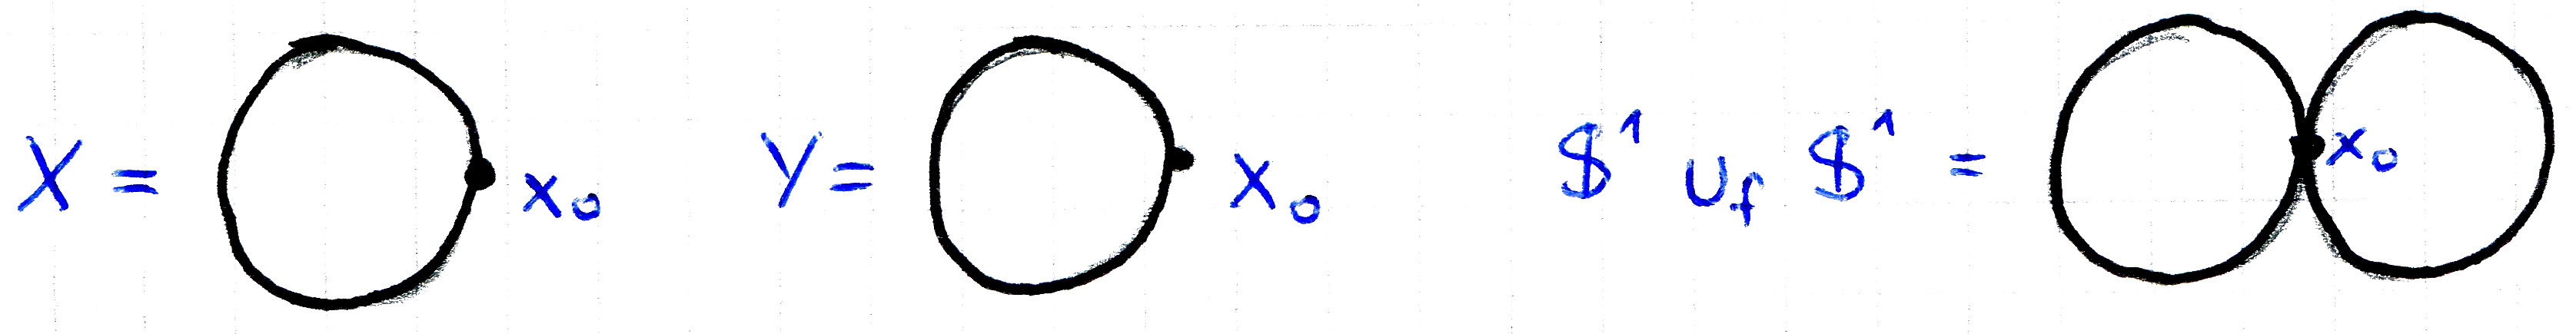
\includegraphics[width=.5\textwidth]{EinfacheVerklebung}
        \caption{Einfache Verklebung}
      \end{figure}
    \item \( X = [0,1] \), \( Y = [2,5] \), \( A = \{ 0,1 \} \subset X \), \( f(0) = 2 \), \( f(1) = 3 \)
    \begin{figure}[H]
      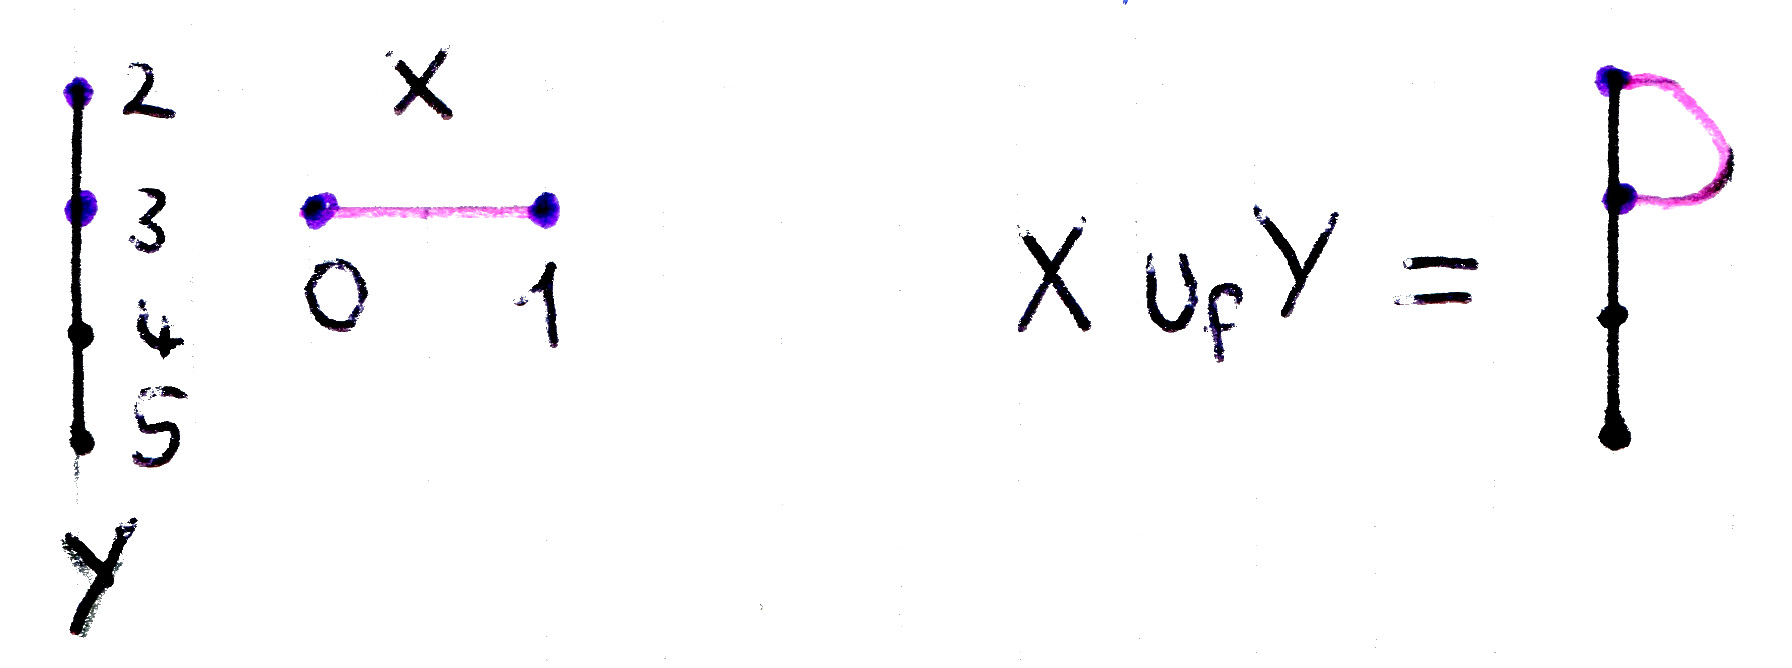
\includegraphics[width=.5\textwidth]{Intervallverklebung}
      \caption{Intervallverklebung}
    \end{figure}
    \item \emph{Zusammenhängende Summe} von \( 2 \)-Mannigfaltigkeiten \( M_1 \) und \( M_2 \).
      \begin{figure}[H]
        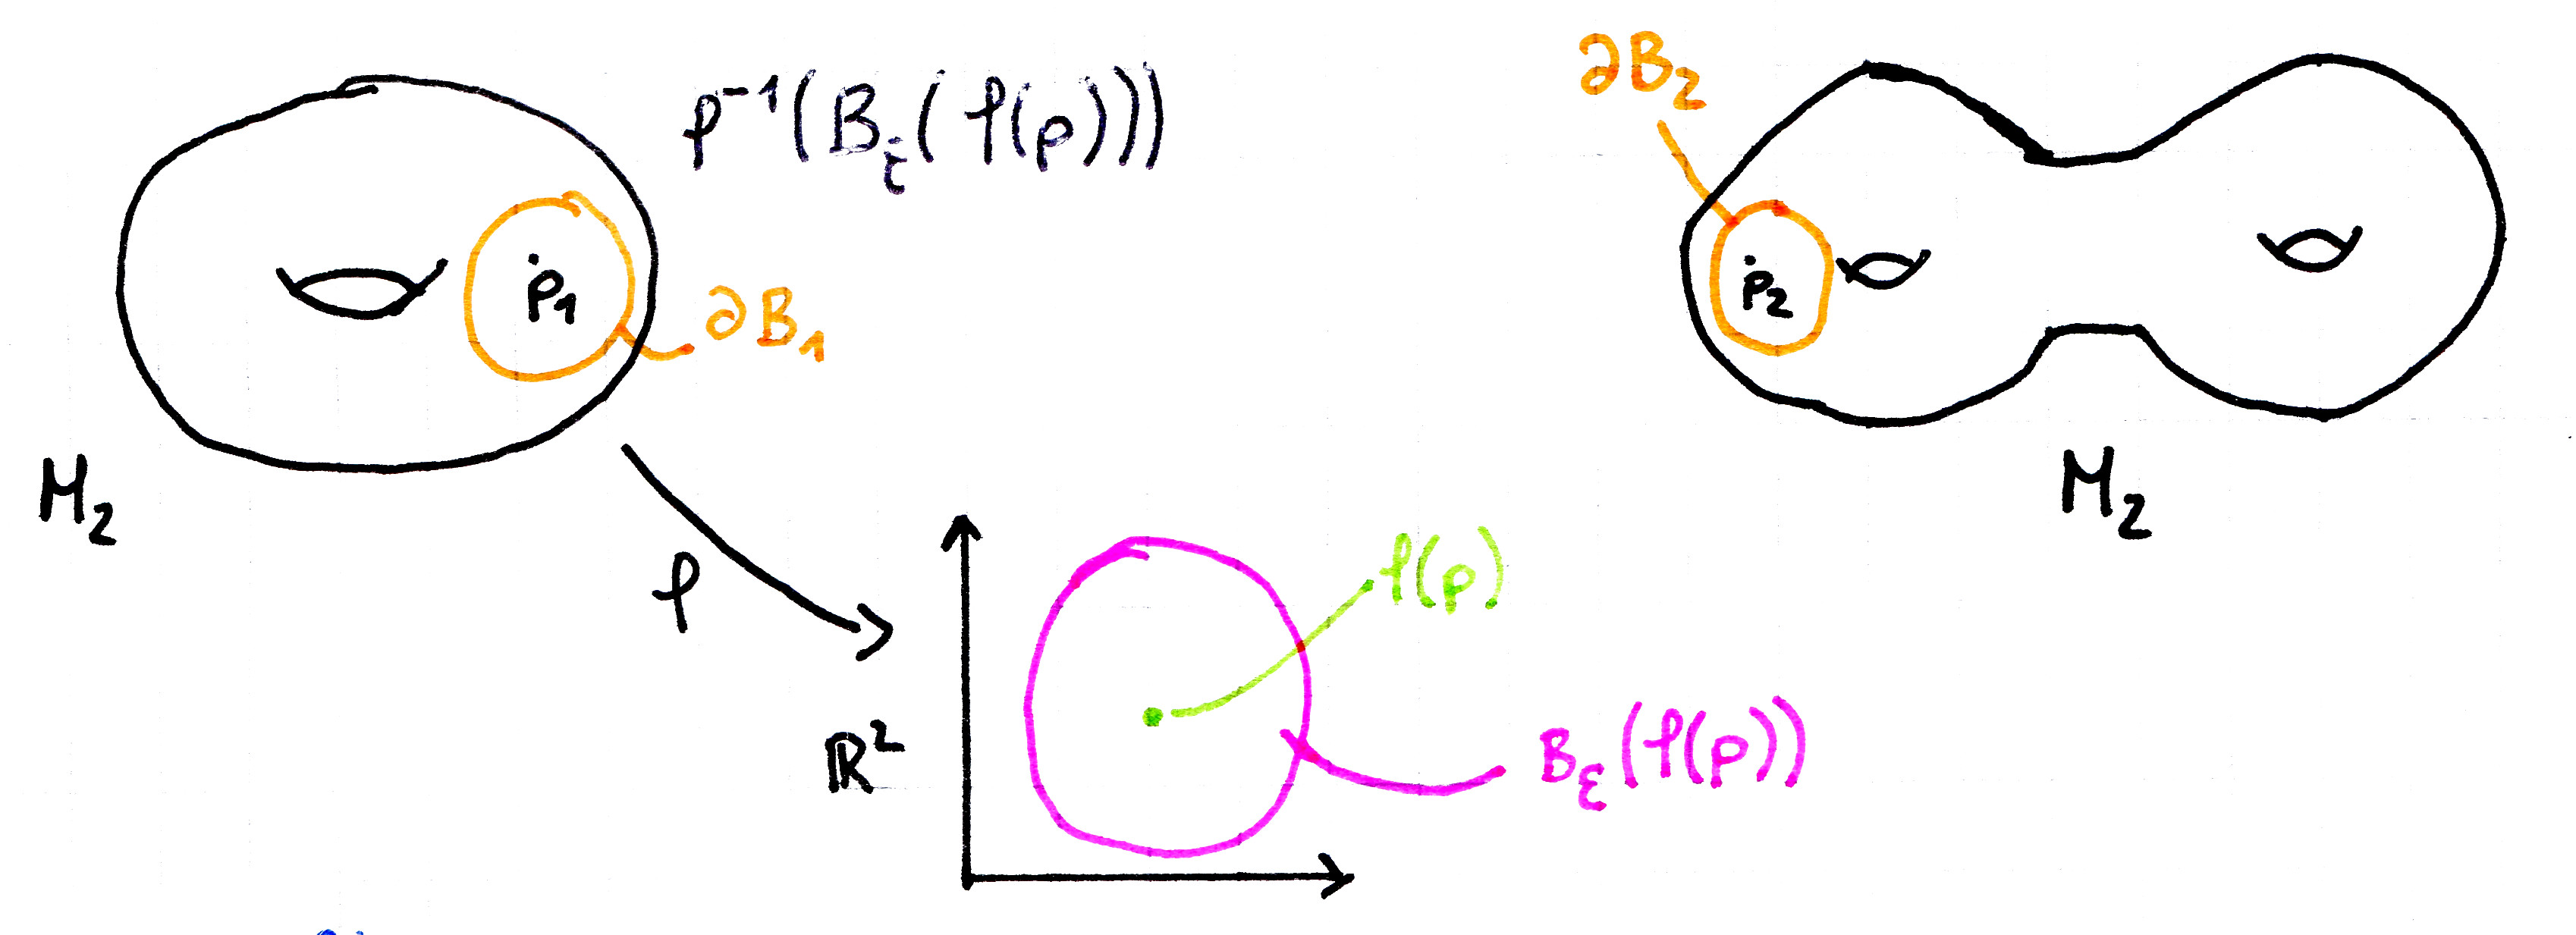
\includegraphics[width=.8\textwidth]{ZusammenhaengendeSumme}
        \caption{Zusammenhängende Summe von \( 2 \)-Mannigfaltigkeiten}
      \end{figure}
      Konstruktion:
      \begin{enumerate}
        \item Entferne geeignet kleine abgeschlossene ``Kreisscheiben'' von \( p_1 \in M_1 \) und \( p_2 \in M_2 \) mit Rändern \( \delta B_1 \) und \( \delta B_2 \) Homöomorph zu \( S^1 \).
        \item Wähle Homöomorphismus \( f: \delta B_1 \to \delta B_2 \).
        \item Verklebe \( M_1 \) und \( M_2 \) mittels \( f : M_1 \cup_f M_2 \eqqcolon M_1 \# M_2 \)
        \begin{figure}[H]
          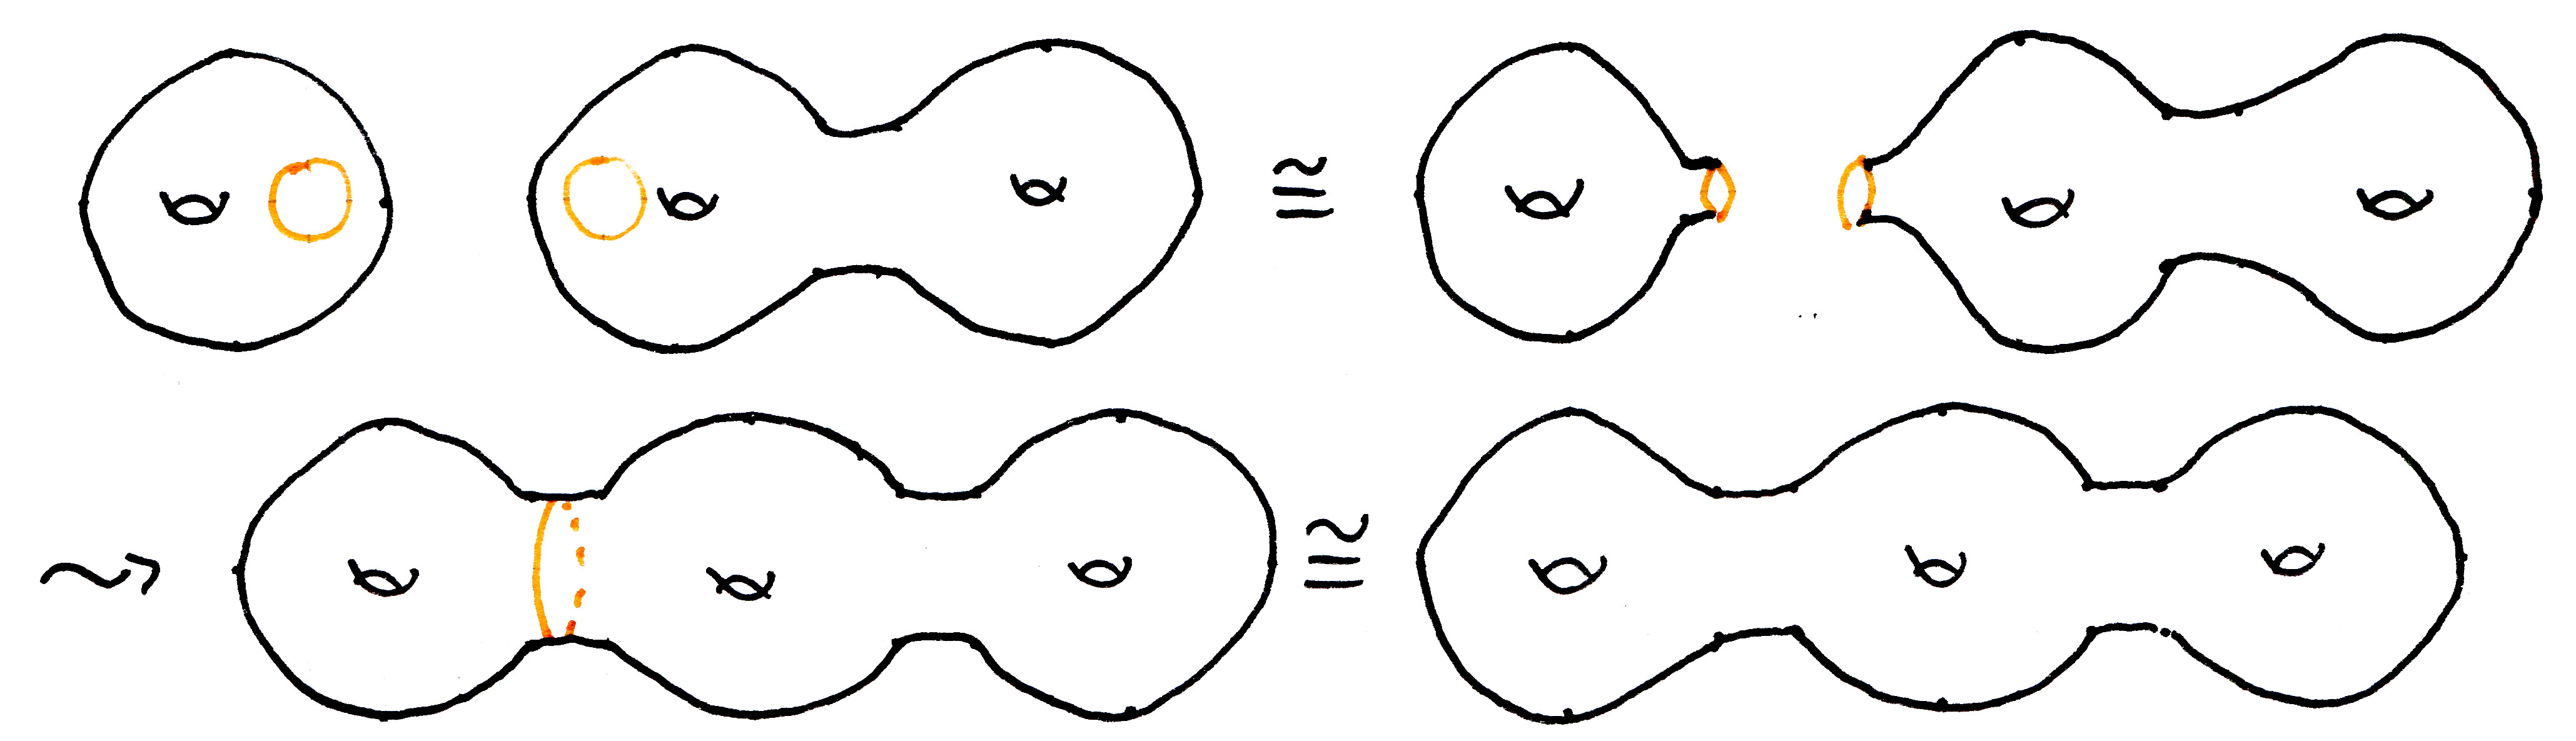
\includegraphics[width=.8\textwidth]{Verklebung}
          \caption{Verklebung}
        \end{figure}
      \end{enumerate}
      Alle kompakten geschlossenen Flächen kann man aus \( S^2 \) konstruieren durch Verkleben Tori.
      \begin{figure}[H]
        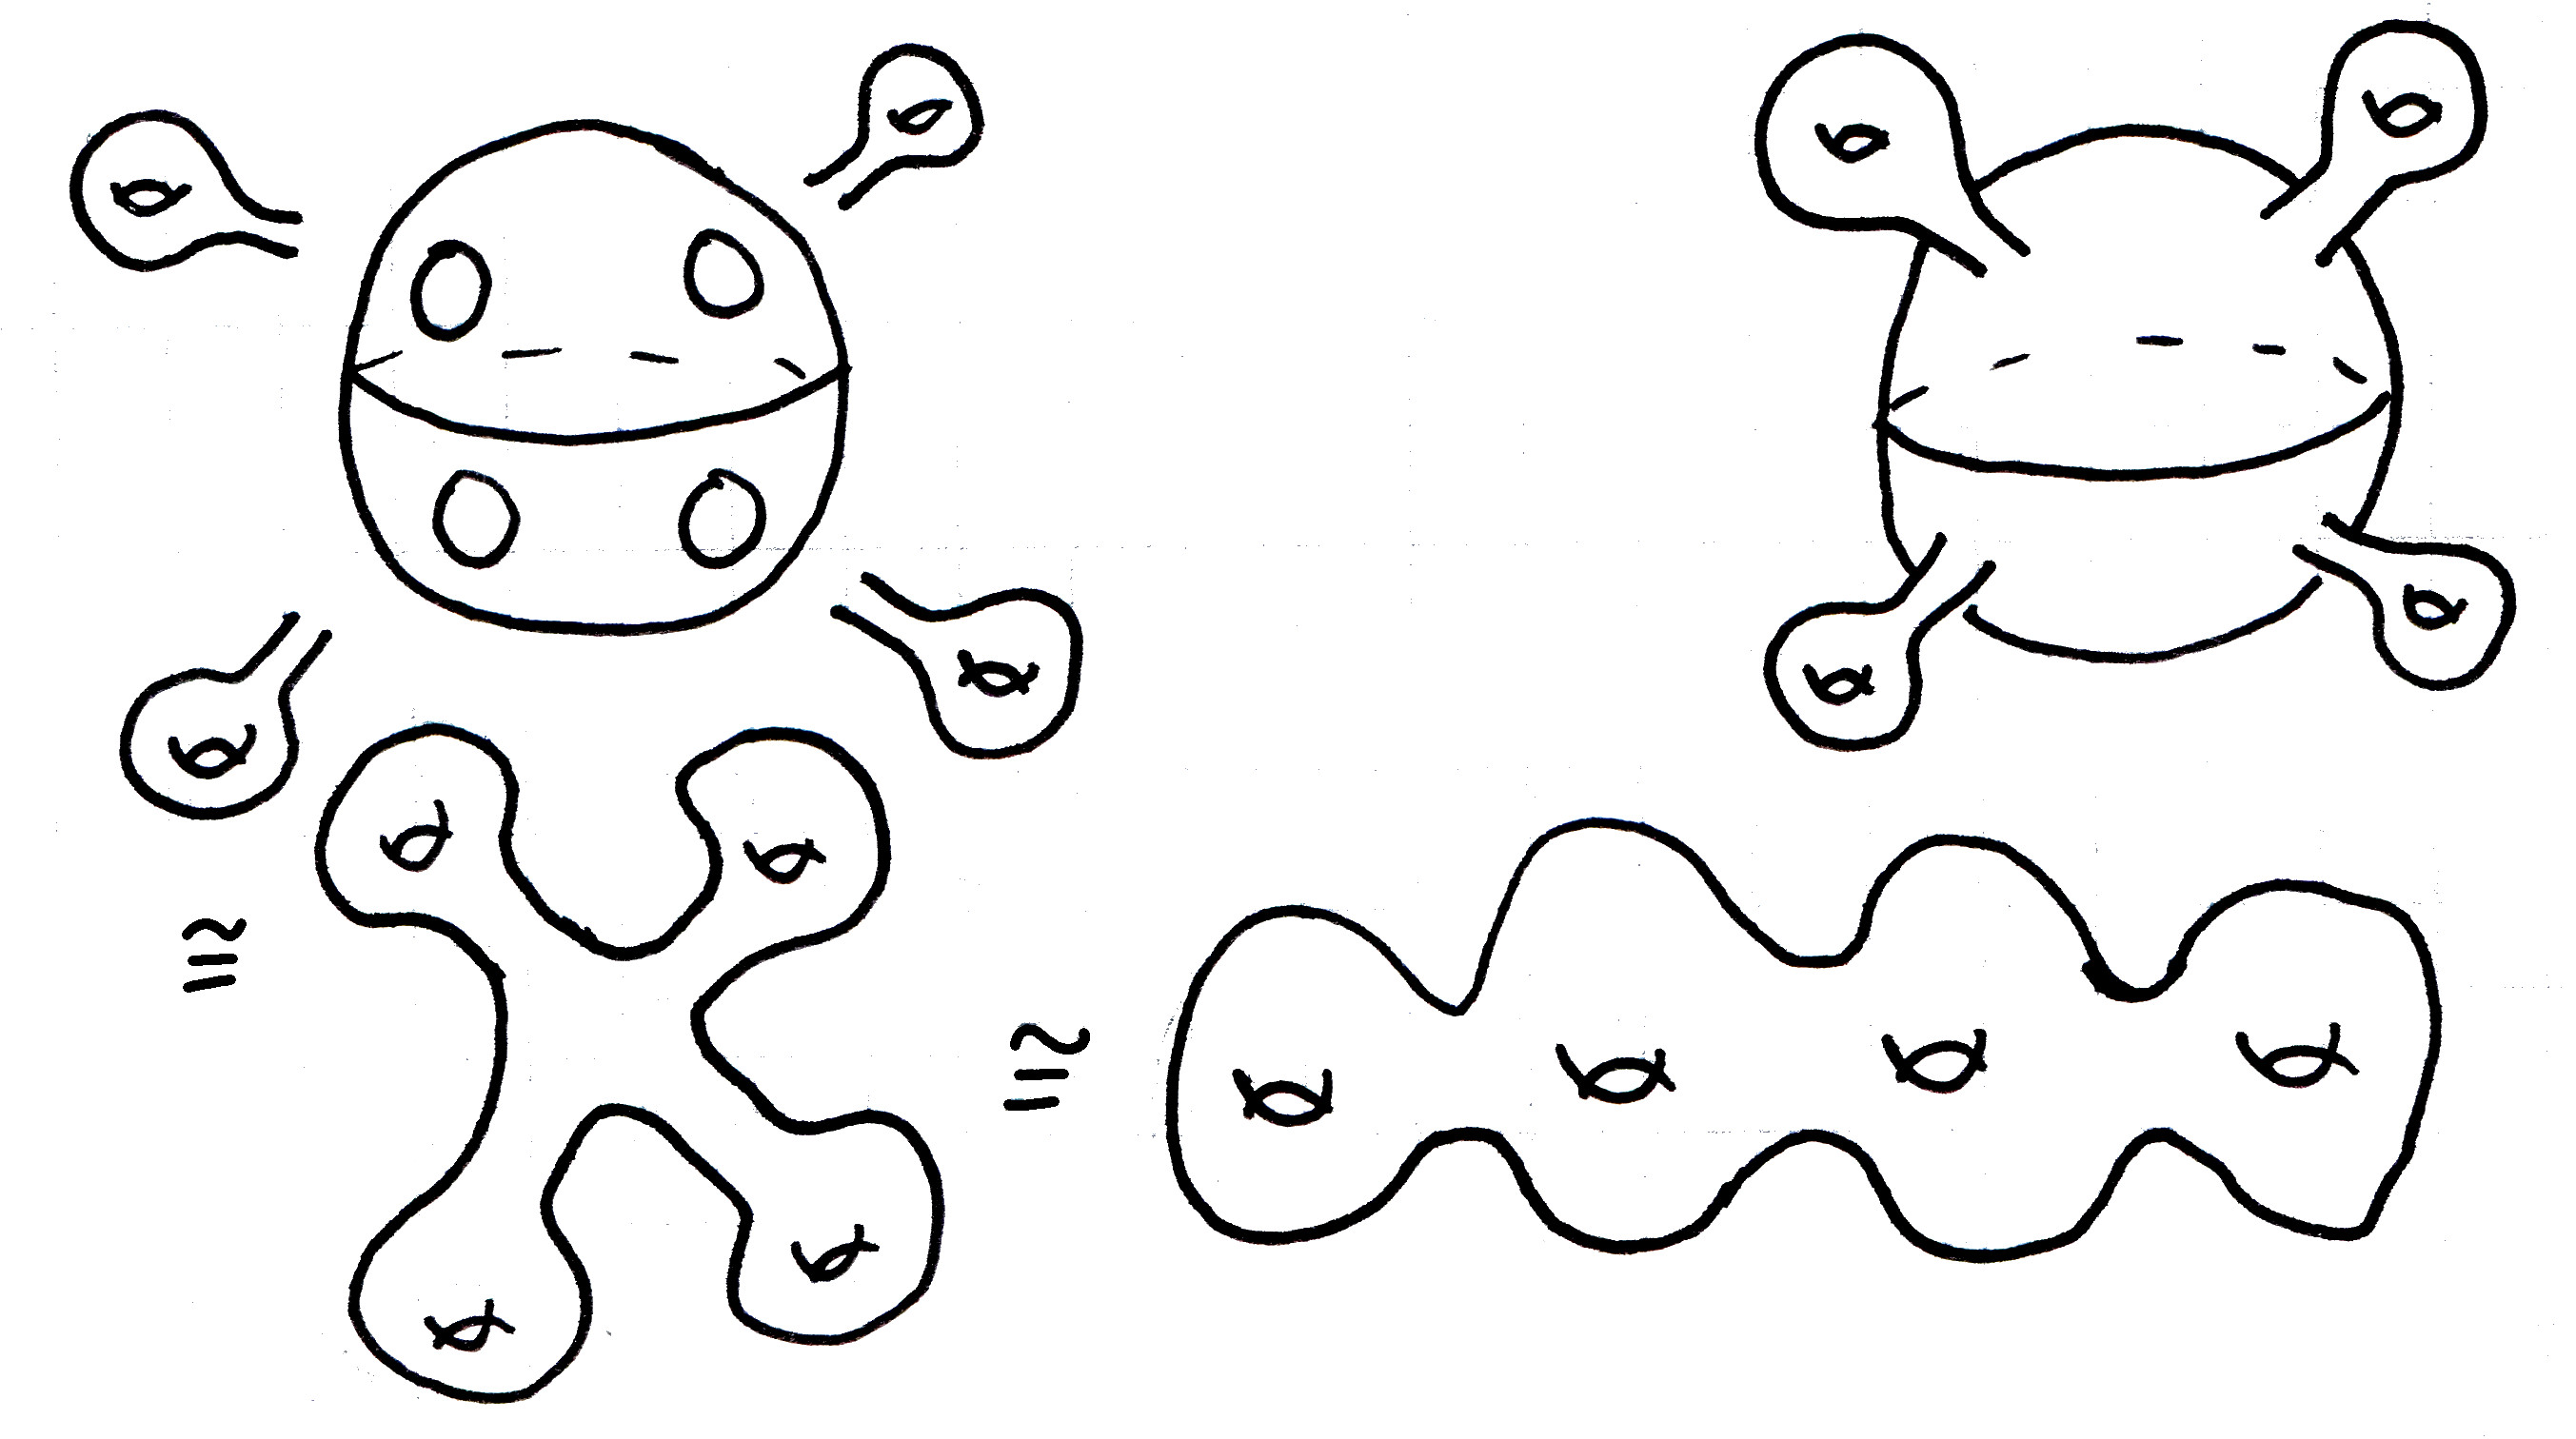
\includegraphics[width=.5\textwidth]{BeliebigeGeschlosseneFlaeche}
        \caption{Konstruieren einer beliebigen kompakten geschlossenen Fläche aus \( S^2 \)}
      \end{figure}
  \end{enumerate}
\end{example}

\begin{remark}[Selbstverklebungen]
  ``\term{Selbst-Verklebungen}''\label{def:selbstverklebung} sind analog definiert: \\
  \( X = \) topologischer Raum, \( A \subset X \) Teilraum, \( f : A \to X \), \( X_f \coloneqq X/_\sim \) mit Äquivalenzrelation wie oben.
\end{remark}

\begin{example}
  \
  \begin{enumerate}
    \item \( X = [0,1] \times [0,1] \) = Einheitsquadrat,

      \begin{minipage}{.45\textwidth}
        \begin{align*}
          A \subset \delta X = &\underbrace{\left( \{ 0 \} \times [0,1] \right)}_{\eqqcolon A_1} \cup \underbrace{\left( \{ 1 \} \times [0,1] \right)}_{\eqqcolon B_2} \\
          &\cup \underbrace{\left( [0,1] \times \{ 0 \} \right)}_{\eqqcolon A_2} \cup \underbrace{\left( [0,1] \times \{ 1 \} \right)}_{\eqqcolon B_2}\text{,}
        \end{align*}
      \end{minipage}
      \hfill
      \begin{minipage}{.45\textwidth}
        \begin{figure}[H]
          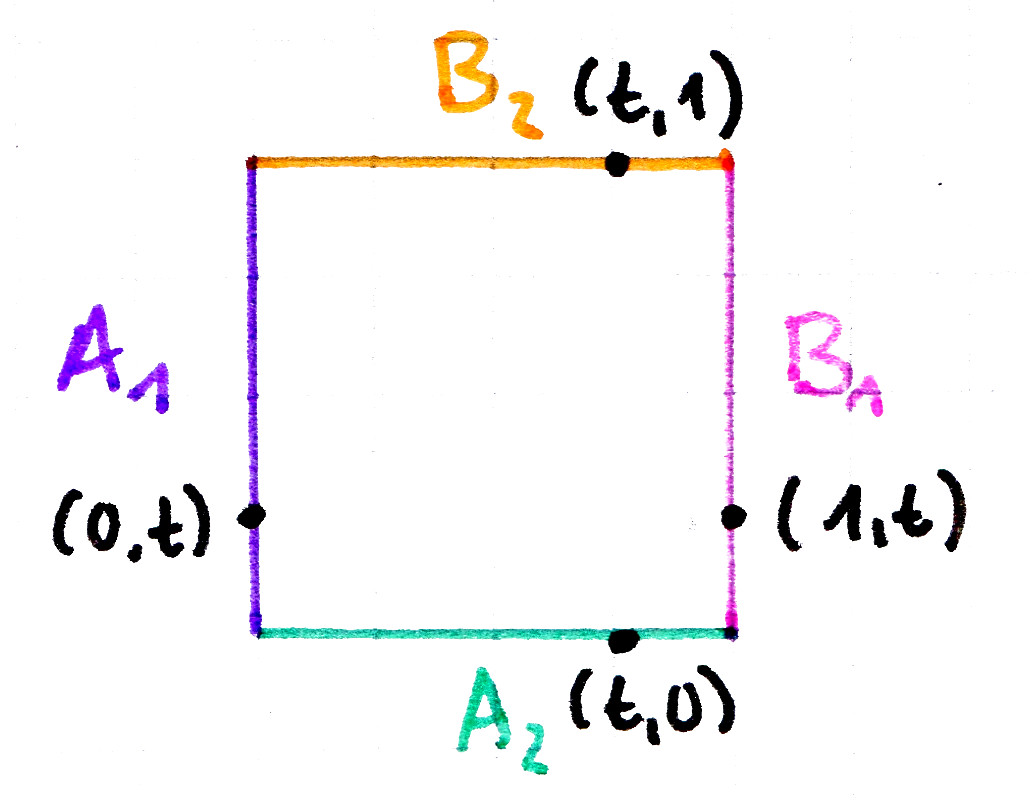
\includegraphics[width=.8\textwidth]{VorbereitungVerklebungEinheitsquadrat}
          \caption{Vorbereitung zur Selbstverklebung am Einheitsquadrat}
        \end{figure}
      \end{minipage}

      \( A \coloneqq A_1 \cup A_2 \),
      \begin{align*}
        f: &A_1 \to B_1, \quad (0,t) \mapsto (1,t) \\
         &A_2 \to B_2, \quad (t,0) \mapsto (t,1)
      \end{align*}
      \begin{figure}[H]
        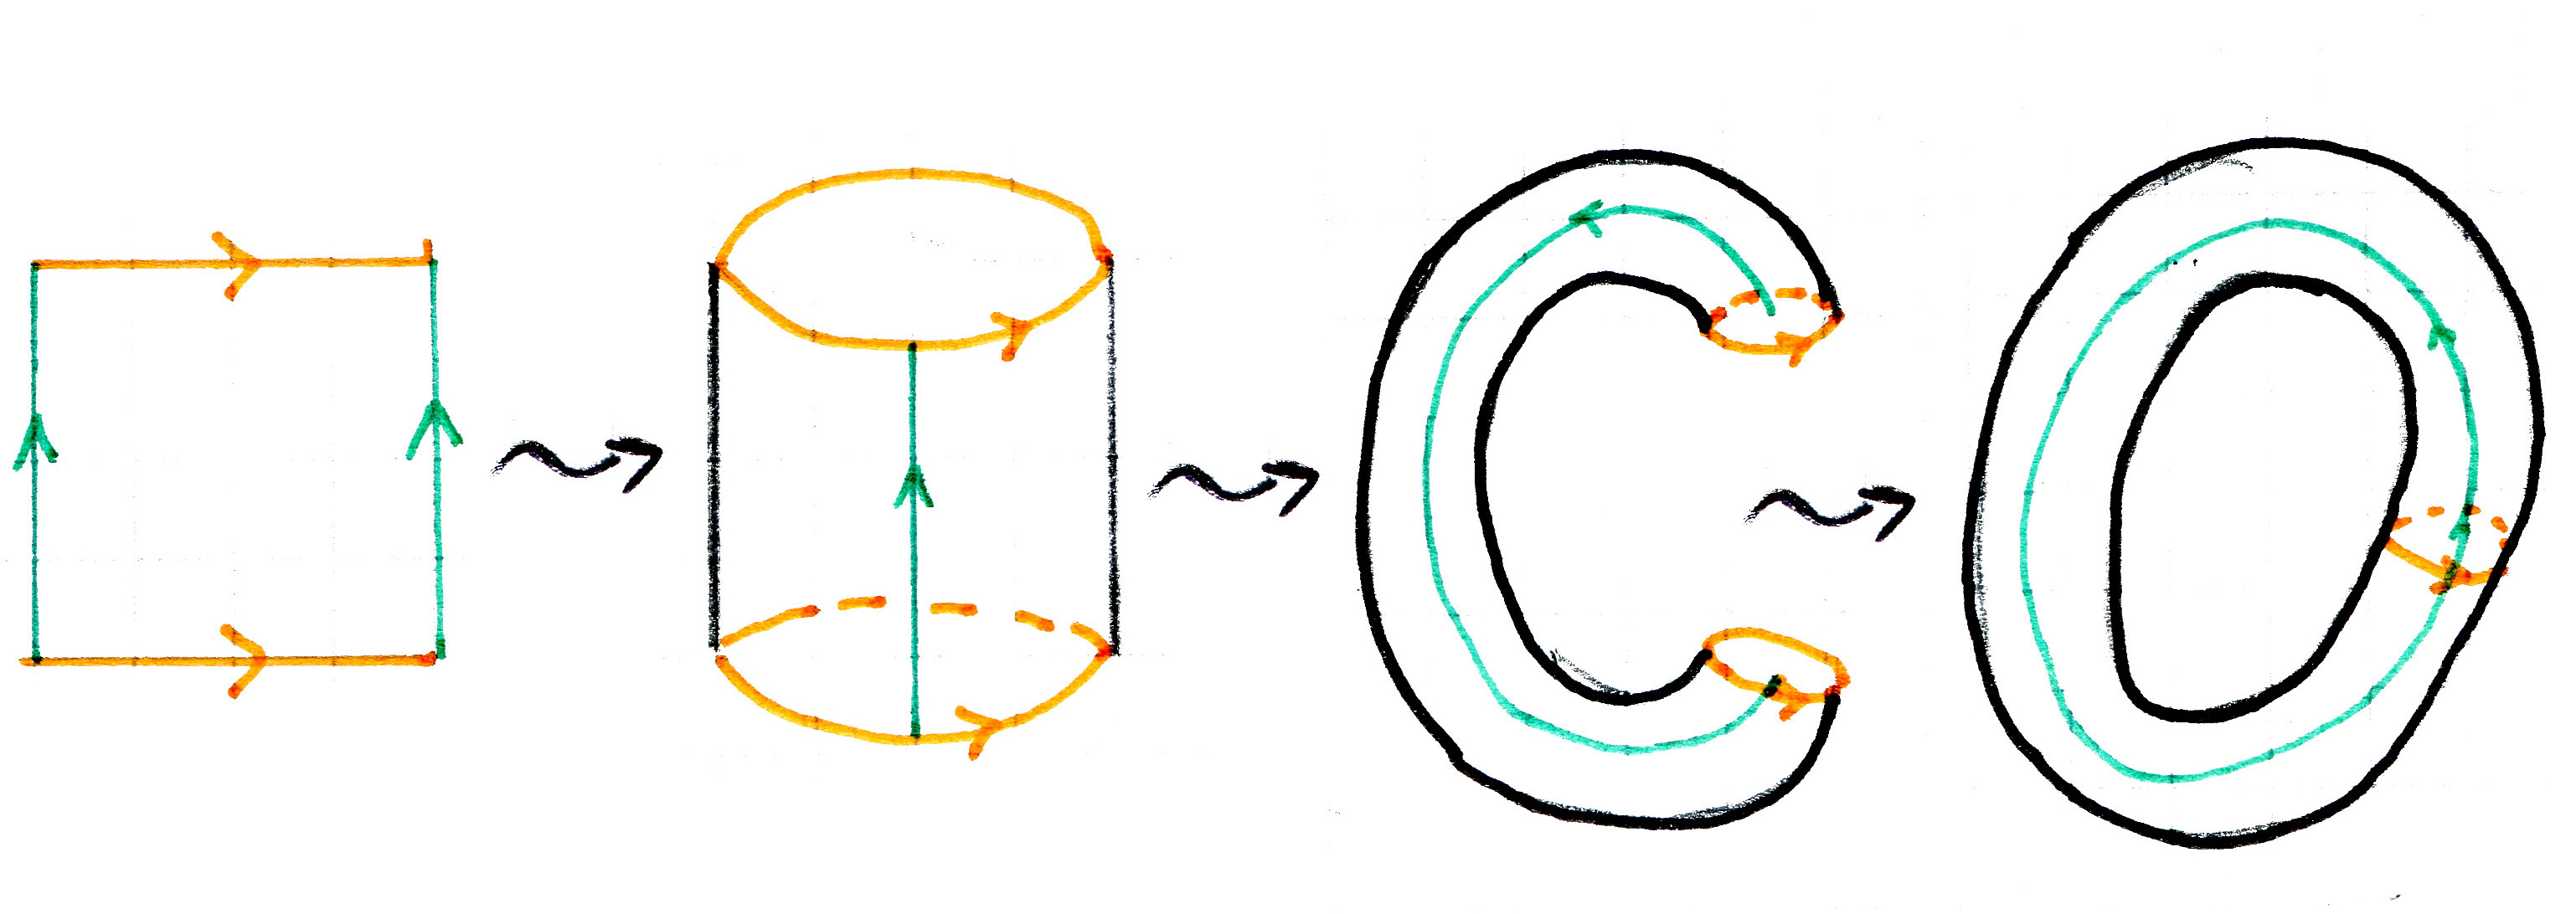
\includegraphics[width=.8\textwidth]{Verklebungsprozess}
        \caption{Verklebungsprozess}
      \end{figure}
    \item \emph{Möbiusband}: \( X = [0,1] \times [0,1] \), \( A = A_1 \), \( f: A_1 \ni (0,1) \mapsto (1,1-t) \in B_1 \)
    % TODO BSP7
    \item \emph{Projektive Ebene}: \( P^2\R \) entsteht durch Verkleben einer Kreisscheibe und eines Möbiusbandes längs der Ränder.
    % TODO BSP8
    % TODO BSP9 --- Kleinsche Flasche
  \end{enumerate}
\end{example}

  \chapter{Geometrie von Flächen}

Ziel dieses Kapitels ist es, auf zweidimensionalen Mannigfaltigkeiten (beziehungsweise Flächen im $ \R^3 $) ``Geometrie'' zu betreiben  (also beispielsweise Längen und Winkel messen und so weiter).\footnote{Für mehr Informationen: \textbf{Gauß} (1827) vgl. \textbf{Spirak}: \emph{A comprehensive introduction to differential geometry} Vol. III --- how to read Gauß}

\section{Reguläre Flächen in $ \R^3 $}

\begin{remark}[Erinnerung an reguläre Flächen]
  Eine Teilmenge $ S \subset \R^3 $ ist eine \term{reguläre Fläche}, falls es zu jedem Punkt $ p \in S $ eine offene Umgebung $ V $ von $ p $ in $ \R^3 $, eine offene Teilmenge $ U \subset \R^2 $ und eine $ C^\infty $-Abbildung
  \begin{equation*}
    x: U \ni (u,v) \mapsto x(u,v) = \left( x_1(u,v),x_2(u,v),x_3(u,v) \right) \in \R^3
  \end{equation*}
  gibt mit:
  \begin{enumerate}
    \item $ x(U) = S \cap V $ und $ x: U \to S \cap V $ ist ein Homöomorphismus. 
    \item Das Differenzial $ \text{d}x|_{(u,v)}: \underset{\cong \R^2}{T_{(u,v)}\R^2} \to \underset{\cong \R^3}{T_{x(u,v)}\R^3} $ ist injektiv ($ \forall (u,v) \in U $)
    \begin{itemize}
      \item[$ \Leftrightarrow $] Die Funktionalmatrix
        \begin{equation*}
          \begin{pmatrix}
            \frac{\partial x_1}{\partial u}(u,v) & \frac{\partial x_1}{\partial v}(u,v) \\
            \frac{\partial x_2}{\partial u}(u,v) & \frac{\partial x_2}{\partial v}(u,v) \\
            \frac{\partial x_3}{\partial u}(u,v) & \frac{\partial x_3}{\partial v}(u,v)
          \end{pmatrix} \eqqcolon \begin{pmatrix}
            x_u(u,v) & x_v(u,v)
          \end{pmatrix}
        \end{equation*}
        hat Rang $ 2 $ ($ \forall (u,v) \in U $).
      \item[$ \Leftrightarrow $] $ x_u(u,v) $, $ x_v(u,v) $ sind linear unabhängig ($ \forall (u,v) \in U $).
      \item[$ \Leftrightarrow $] Vektorprodukt $ x_u(u,v) \times x_v(u,v) \neq 0 $ ($ \forall (u,v) \in U $).
    \end{itemize}
  \end{enumerate}
\end{remark}

\begin{remark}[Erinnerung an das Kreuz-/Vektorprodukt]
  \ \\
  $ a \coloneqq (a_1, a_2, a_3) \in \R^3 $ und $ b \coloneqq (b_1, b_2, b_3) \in \R^3 $.
  \begin{equation*}
    a \wedge b \ (\cong a \times b) \ \coloneqq (a_2b_3-a_3b_2, a_3b_1-a_1b_3, a_1b_2-a_2b_1) \in \R^3\text{.}
  \end{equation*}
  \emph{Eigenschaften}:
  \begin{enumerate}
    \item $ a \wedge b \bot a $ \quad $ a \wedge b \bot b $ 
    \item $ \det(a, b, a \wedge b) \geq 0 $
    \item $ a \wedge (-b) = - (a \wedge b) $
    \item $ \Vert a \wedge b \Vert = \Vert a \Vert * \Vert b \Vert * \sin \alpha $ (Winkel zwischen den Vektoren), Fläche des von $ a $ und $ b $ aufgespannten Parallelogramms
  \end{enumerate}
\end{remark}

\begin{definition}[Tangentialraum]
  Der \term{Tangentialraum}\label{def:tangentialraum} in Punkt $ p \in \R^3 $ ist der affine Unterraum
  \begin{equation*}
    T_p\R^3 \coloneqq \{ p \} \times \R^3 = \{ (p,v) : v \in \R^3 \}\text{.}
  \end{equation*}
  Für eine reguläre Fläche $ S $ und $ p = x(u,v) \in S $ ist die \term{Tangentialebene}\label{def:tangentialebene} in $ p \in S $ definiert als
  \begin{equation*}
    T_pS \coloneqq \text{d}x_{(u,v)}\left(T_{(u,v)}\R^2\right) \coloneqq \{ p \} \times [x_u(u,v), x_v(u,v)] \subset T_p\R^3
  \end{equation*}
  $ 2 $-dimensionaler, affiner Unterraum des $ \R^3 $.
\end{definition}

\begin{remark}[Geometrische Interpretation des Tangentialraums]
  \
  % TODO Grafik einfügen
  \begin{equation*}
    x_u(u_0,v_0) = \frac{\partial x}{\partial u}(u_0,v_0) = \frac{\text{d}}{\text{d}t}|_{t = 0}x(u_0+t,v_0) = \text{d}x|_{(u_0,v_0)}(e_1)
  \end{equation*}
  \emph{Allgemein}: \\*
  Sei $ c(t) \coloneqq x(u(t),v(t)) $ eine \term{Flächenkurve}\label{def:flaechenkurve} in $ x(U) $ durch den Punkt $ x(u(0),v(0)) = x(u_0,v_0) $. \\*
  \term{Tangentialvektor}\label{def:tangentialvektor} an $ c $ im Punkt $ x(u_0,v_0): $
  \begin{align*}
    c'(0) &= \frac{\text{d}c}{\text{d}t}|_{t=0} = \frac{\text{d}}{\text{d}t}x(u(t),v(t))|_{t = 0} \\
      &= \frac{\partial x}{\partial u}(u(0),v(0))u'(0) + \frac{\partial x}{\partial v}v'(0) = x_u(u_0,v_0)u'(0)+x_v(u_0,v_0)v'(0)
  \end{align*}
  \emph{Also}: Tangentialebene in $ x(u_0,v_0) = $ Menge aller Tangentialvektoren als Flächenkurven.
\end{remark}

\begin{remark}[Parameterisierungsunabhängigkeit obiger Definitionen]
  \ \\
  Sei $ \overline{x} : \overline{U} \to \overline{x}(\overline{U}) = x(U) $ eine andere Parametrisierung von $ S $ um $ p = x(u_0, v_0) = \overline{x}(\overline{u_0}, \overline{v_0}) $. \\
  \emph{Zu zeigen}: Die lineare Hüllen sind gleich: $ [\overline{x}_{\overline{u}}, \overline{x}_{\overline{v}}] = [x_u, x_v] $. \\
  Es ist $ k \coloneqq \overline{x}^{-1}*x : U \to \overline{U} $ die Koordinatentransformation:
  \begin{equation*}
    x_u = \frac{\partial x}{\partial u}(u,v) = \frac{\partial \overline{x}(\overline{x}^{-1} \circ x)}{\partial u}(u,v) = \frac{\partial \overline{x}}{\partial u}(\overline{u}, \overline{v}) = \frac{\partial \overline{x}}{\partial \overline{u}}(\overline{u},\overline{v}) *\frac{\partial \overline{u}}{\partial u}(u,v)+\frac{\partial \overline{x}}{\partial \overline{v}} * \frac{\partial \overline{v}}{\partial u}
  \end{equation*}
  Entsprechend:
  \begin{align*}
    x_u &= \overline{x}_{\overline{u}}\frac{\partial \overline{u}}{\partial u} + \overline{x}_{\overline{v}}\frac{\partial \overline{v}}{\partial u} \quad \text{d.h. $ x_u $ ist Linearkombination von $ \overline{x}_{\overline{u}} $ und $ \overline{x}_{\overline{v}} $} \\
    x_v &= \overline{x}_{\overline{u}}\frac{\partial \overline{u}}{\partial v} + \overline{x}_{\overline{v}}\frac{\partial \overline{v}}{\partial v} \quad \text{d.h. $ x_v $ ist Linearkombination von $ \overline{x}_{\overline{u}} $ und $ \overline{x}_{\overline{v}} $}
  \end{align*}
  Also $ [x_u, x_v] = [\overline{x}_{\overline{u}}, \overline{x}_{\overline{v}}] $, verschiedene Basen von $ T_pS $ mit Basis-Transformations-Matrix
  \begin{equation*}
    D(u,v) = \begin{pmatrix}
      \frac{\partial \overline{u}}{\partial u} & \frac{\partial \overline{u}}{\partial v} \\
      \frac{\partial \overline{v}}{\partial u} & \frac{\partial \overline{v}}{\partial v}
    \end{pmatrix}\text{.}
  \end{equation*}
  Das ist die Funktionalmatrix der Parametertransformation. Insb. ist $ \det D(u,v) \neq 0 $.
\end{remark}

\begin{example}
  \
  \begin{enumerate}
    \item \emph{affine Ebene}: $ a_0, a, b \in \R^3 $, $ S \coloneqq \{ a_0 + ua + vb : u,v \in \R \} $ ist reguläre Fläche, falls $ a $ und $ b $ linear unabhängig sind. Mit
    \begin{equation*}
      U \coloneqq \R^2, \ V \coloneqq \R^3, \ x: \R^2 \ni (u,v) \mapsto a_0 + ua + vb \in \R^3\text{,}
    \end{equation*}
    \begin{equation*}
      x_u  =\frac{\partial x}{\partial u} = a, \ x_v = \frac{\partial x}{\partial v} = b, \ T_{x(u,v)}S = \{ x(u,v) \} \times [a,b] \cong S\text{.}
    \end{equation*}

    \item $ U \subseteq \R^2 $, $ f: U \to \R $ $ C^\infty $-Funktion, $ S \coloneqq $ Graph von $ f \coloneqq \{ (x_1, x_2, x_3) \in \R^3 : (x_1, x_2) \in U, \ x_3 = f(x_1, x_2) \} $. \\
    \emph{Behauptung}: $ S $ ist reguläre Fläche. \\
    $ U = U $, $ V = \R^3 $, $ x : U \ni (u,v) \mapsto (u,v, f(u,v)) \in \R^3 $. \\
    $ x(U) = S = S \cap V $, $ x: U \to S $ stetig und $ x^{-1}: S \ni (u,v,f(u,v)) \mapsto (u,v) \in U $ ist als Projektion auch stetig. Also ist $ x $ ein Homöomorphismus. \\
    Weiter ist
    \begin{align*}
      x_u &= \left(1,0, \frac{\partial f}{\partial u}\right), \\
      x_v &= \left( 0,1, \frac{\partial f}{\partial v} \right)
    \end{align*}
    also sind $ x_u $ und $ x_v $ linear unabhängig.
  \end{enumerate}
\end{example}

\begin{remark}
  Ist $ S $ reguläre Fläche in $ \R^3 $, so existiert zu jedem Punkt $ p \in S $ eine offene Umgebung $ O \subset \R^3 $, so dass $ S \cap O $ Graph einer $ C^\infty $-Funktion ist (beispielsweise $ S^2 = $ 2-Sphäre vom Radius $ 1 $).
\end{remark}

\section{Erste Fundamentalform einer regulären Fläche}

\begin{remark}[Erinnerung an LA]
  Modell der euklidischen Geometrie: \\*
  $ \R $-Vektorraum + Skalarprodukt = euklidischer $ (V, \langle \cdot, \cdot \rangle) $-Vektorraum \\*
  $ \leadsto \Vert a \Vert = \sqrt{\langle a, a \rangle} $ \textbf{Länge} eines Vektors $ a \in V $ \\*
  $ \leadsto \cos \measuredangle(a,b) = \frac{\langle a, b \rangle}{\Vert a \Vert*\Vert b \Vert} = \left\langle \frac{a}{\Vert a \Vert}, \frac{b}{\Vert b \Vert} \right\rangle $ \textbf{Winkel} \\
\end{remark}

\begin{remark}[Übertragung auf gekrümmte Flächen (Gauß)]
  Sei $ S $ eine reguläre Fläche und $ p \in S $. Betrachte die bilineare Abbildung
  \begin{equation*}
    \langle \cdot, \cdot \rangle_p : T_pS \times T_pS \to T_pS\text{,} \quad \langle a, b \rangle_p \coloneqq \langle a, b \rangle
  \end{equation*}
  (identifiziere affine Ebene mit VR $ R^2 $, $ \langle a, b \rangle $ ist Standard-SKP in $ \R^3 $). \\
  Die Zuordnung $ I: p \mapsto I_p \coloneqq \langle \cdot, \cdot \rangle_p $ heißt \term{1. Fundamentalform der Fläche $ S $}\label{def:ersteFundamentalform}. \\
  Ist $ x: U \ni (u,v) \mapsto x(u,v) \in S $ eine lokale Parametrisierung von $ S $ (um $ p \in S $), so bilden $ x_u(u,v) $ und $ x_v(u,v) $ eine Basis von $ T_{x(u,v)}S $. Bezüglich dieser können wir $ I_p $, $ p \in x(U) \subset S $ durch eine positiv definite symmetrische $ 2 \times 2 $-Matrix darstellen:
  \begin{equation*}
      \left( \underbrace{g_{ij}(u,v)}_{\in \R^{2 \times 2}} \right) = \begin{pmatrix}
        g_{11}(u,v) & g_{12}(u,v) \\
        g_{21}(u,v) & g_{22}(u,v)
      \end{pmatrix} = \underset{\text{Originalnotation Gauß}}{\begin{pmatrix}
        E(u,v) & F(u,v) \\
        F(u,v) & G(u,v)
      \end{pmatrix}}
  \end{equation*}
  mit
  \begin{align*}
    g_{11}(u,v) = E(u,v) &= \langle x_u(u,v),x_u(u,v) \rangle_p = \underset{\text{Standard-SKP von }\R^3}{\langle x_u(u,v),x_u(u,v) \rangle} \\
    g_{12}(u,v) &= \langle x_u, x_v \rangle_p = \langle x_v, x_u \rangle = g_{21}(u,v) \\
    g_{22}(u,v) &= \langle x_v, x_v \rangle_p = \langle x_v, x_v \rangle
  \end{align*}
  insbesondere sind die $ g_{ij}: U \to \R $ $ C^\infty $-Funktionen. \\
  \emph{Also}: $ \left( g_{ij}(u,v) \right) $ ist eine Familie $ \in \R^{2\times 2} $ von Skalarprodukten, die differenzierbar von $ (u,v) $ abhängig ist. (Riemannsche Metrik)
\end{remark}

\begin{remark}[Bedingungen an obige Matrix]
  \
  \begin{enumerate}
    \item \emph{Hurwitz}: $ I_p $ ist positiv definit $ \Leftrightarrow E = g_{11} > 0 $, $ E*G-F^2 = \det(g_{ij}) > 0 $.
    \item \emph{andere Parametrisierung}: $ \overline{x}(\overline{u},\overline{v}) \leadsto $ neue Basis $ \{ \overline{x}_{\overline{u}}, \overline{x}_{\overline{v}} \} $, Matrix von $ I $ bezüglich dieser Basis $ \left( \underset{\in \R^{2\times 2}}{\overline{g}_{ij}(\overline{u}, \overline{v})} \right) $ mit
    \begin{equation*}
      \left( g_{ij}(u,v) \right) = D(u,v)^\top(\overline{g}_{ij}(\overline{u},\overline{v}))D(u,v)
    \end{equation*}
    mit 
    \begin{equation*}
      D(u,v) = \begin{pmatrix}
        \frac{\partial \overline{u}}{\partial u} & \frac{\partial \overline{u}}{\partial v} \\
        \frac{\partial \overline{v}}{\partial u} & \frac{\partial \overline{v}}{\partial v}
      \end{pmatrix}\text{,}
    \end{equation*}
    siehe auch Basiswechselmatrix.
  \end{enumerate}
\end{remark}

\end{document}
